% !Mode:: "TeX:UTF-8"
% !TEX encoding = UTF-8 Unicode

%----------------------------------------------------------------------------------------
% 机器翻译:基础与模型
% Machine Translation: Foundations and Models
%
% Copyright 2020
% 肖桐(xiaotong@mail.neu.edu.cn) 朱靖波 (zhujingbo@mail.neu.edu.cn)
%----------------------------------------------------------------------------------------

%----------------------------------------------------------------------------------------
%    CONFIGURATIONS
%----------------------------------------------------------------------------------------

\renewcommand\figurename{图}%将figure改为图
\renewcommand\tablename{表}%将figure改为图
\chapterimage{fig-NEU-7.jpg} % Chapter heading image

%----------------------------------------------------------------------------------------
%	CHAPTER 16
%----------------------------------------------------------------------------------------
\chapter{低资源神经机器翻译}

\parinterval 神经机器翻译带来的性能提升是显著的,但随之而来的问题是对海量双语训练数据的依赖。不同语言可使用的数据规模是不同的。比如汉语、英语这种使用范围广泛的语言,存在着大量的双语平行句对,这些语言被称为{\small\bfnew{富资源语言}}\index{富资源语言}(High-resource Language\index{High-resource Language})。而对于其它一些使用范围稍小的语言,如斐济语、古吉拉特语等,相关的数据非常稀少,这些语言被称为{\small\bfnew{低资源语言}}\index{低资源语言}(Low-resource Language\index{Low-resource Language})。世界上现存语言超过5000种,仅有很少一部分为富资源语言,绝大多数均为低资源语言。即使在富资源语言中,对于一些特定的领域,双语平行语料也是十分稀缺的。有时,一些特殊的语种或者领域甚至会面临“零资源”的问题。因此,{\small\bfnew{低资源机器翻译}}\index{低资源机器翻译}(Low-resource Machine Translation)\index{Low-resource Machine Translation}是当下急需解决且颇具挑战的问题。

\parinterval 本章将对低资源神经机器翻译的相关问题、模型和方法展开介绍,内容涉及数据的有效使用、双向翻译模型、多语言翻译模型、无监督机器翻译、领域适应五个方面。

%----------------------------------------------------------------------------------------
%    NEW SECTION 16.1
%----------------------------------------------------------------------------------------

\section{数据的有效使用}\label{effective-use-of-data}

\parinterval 数据稀缺是低资源机器翻译所面临的主要问题,充分使用既有数据是一种解决问题的思路。比如,在双语训练不充足的时候,可以对双语数据的部分单词用近义词进行替换,达到丰富双语数据的目的\upcite{DBLP:conf/acl/FadaeeBM17a,DBLP:conf/emnlp/WangPDN18},也可以考虑用转述等方式生成更多的双语训练数据\upcite{DBLP:conf/emnlp/MartonCR09,DBLP:conf/eacl/LapataSM17}。

\parinterval 另一种思路是使用更容易获取的单语数据。实际上,在统计机器翻译时代,使用单语数据训练语言模型是构建机器翻译系统的关键步骤,好的语言模型往往会带来性能的增益。而这个现象在神经机器翻译中似乎并不明显,因为在大多数神经机器翻译的范式中,并不要求使用大规模单语数据来帮助机器翻译系统。甚至,连语言模型都不会作为一个独立的模块。这一方面是由于神经机器翻译系统的解码端本身就起着语言模型的作用,另一方面是由于双语数据的增多使得翻译模型可以很好地捕捉目标语言的规律。但是,双语数据总是有限的,很多场景下,单语数据的规模会远大于双语数据,如果能够让这些单语数据发挥作用,显然是一种非常好的选择。针对以上问题,下面将从数据增强、基于语言模型的单语数据使用等方面展开讨论。

%----------------------------------------------------------------------------------------
%    NEW SUB-SECTION
%----------------------------------------------------------------------------------------
\subsection{数据增强}

\parinterval {\small\bfnew{数据增强}}\index{数据增强}(Data Augmentation)\index{Data Augmentation}是一种增加训练数据的方法,通常通过对既有数据进行修改或者生成新的伪数据等方式实现。有时候,数据增强也可以被看做是一种防止模型过拟合的手段\upcite{DBLP:journals/jbd/ShortenK19}。在机器翻译中,典型的数据增强方法包括回译、修改双语数据、双语句对挖掘等。

%----------------------------------------------------------------------------------------
%    NEW SUB-SUB-SECTION
%----------------------------------------------------------------------------------------
\subsubsection{1. 回译}

\parinterval {\small\bfnew{回译}}\index{回译}(Back Translation, BT\index{Back Translation})是目前机器翻译任务上最常用的一种数据增强方法\upcite{Sennrich2016ImprovingNM,DBLP:conf/emnlp/EdunovOAG18,DBLP:conf/aclnmt/HoangKHC18}。回译的主要思想是:利用目标语言-源语言翻译模型(反向翻译模型)来生成伪双语句对,用于训练源语言-目标语言翻译模型(正向翻译模型)。假设现在需要训练一个英汉翻译模型。首先,使用双语数据训练汉英翻译模型,即反向翻译模型。然后通过该模型将额外的汉语单语句子翻译为英语句子,从而得到大量的英语- 真实汉语伪双语句对。然后,将回译得到的伪双语句对和真实双语句对混合,训练得到最终的英汉翻译模型。
回译方法只需要训练一个反向翻译模型,就可以利用单语数据来增加训练数据的数量,因此得到了广泛使用\upcite{Hassan2018AchievingHP,DBLP:conf/iclr/LampleCDR18,DBLP:conf/emnlp/LampleOCDR18}。图\ref{fig:16-1} 给出了回译方法的一个简要流程。

%----------------------------------------------
\begin{figure}[htp]
\centering
\begin{tikzpicture}


\tikzstyle{bignode} = [,inner sep=0.3em,draw=black,line width=0.6pt,rounded corners=2pt,minimum width=3.0em]


\node [anchor=center] (node1-1) at (0,0) {\small{汉语}};
\node [anchor=west] (node1-2) at ([xshift=0.8em]node1-1.east) {\small{英语}};
\node [anchor=north] (node1-3) at ([xshift=1.75em]node1-1.south) {\small{反向翻译模型}};
\draw [->,thick](node1-1.east)--(node1-2.west);

\begin{pgfonlayer}{background}
{
\node[fill=blue!20,inner sep=0.3em,draw=black,line width=0.6pt,minimum width=6.0em,drop shadow,rounded corners=2pt] [fit =(node1-1)(node1-2)(node1-3)]  (remark1) {};
}
\end{pgfonlayer}


\node [anchor=north,fill=green!20,bignode](node2-1) at ([yshift=-3em]node1-3.south){\small{汉语}};
\node [anchor=north,fill=green!20,bignode](node2-2) at (node2-1.south){\small{英语}};
\draw [->,thick](node2-1.north)--(remark1.south) node [pos=0.5,right] (pos1) {\small{训练}};


\node [anchor=west,fill=yellow!20,bignode](node3-1) at ([xshift=6.5em,yshift=0.0em]node1-2.east){\small{汉语}};
\node [anchor=north,fill=red!20,bignode](node3-2) at ([yshift=-2.5em]node3-1.south){\small{英语}};
\node [anchor=center](node3-3) at ([xshift=0.4em]node3-2.east){};

\draw [->,thick](node3-1.south)--(node3-2.north) node [pos=0.5,right] (pos2) {\small{翻译}};

\begin{pgfonlayer}{background}
{
\node[rounded corners=2pt,inner sep=0.3em,draw=black,line width=0.6pt,dotted] [fit =(node3-1)(node3-2)(node3-3)]  (remark2) {};
}
\end{pgfonlayer}

\draw [->,thick](remark1.east)--([xshift=5.5em]remark1.east) node [pos=0.5,above] (pos2) {\small{模型翻译}};
\node [anchor=south](pos2-2) at ([yshift=-0.5em]pos2.north){\small{使用反向}};

\draw[decorate,thick,decoration={brace,amplitude=5pt}] ([yshift=1.5em,xshift=1.5em]node3-1.east) -- ([yshift=-8.6em,xshift=1.5em]node3-1.east) node [pos=0.1,right,xshift=0.0em,yshift=0.0em] (label1) {\small{{混合}}};


\node [anchor=west,fill=red!20,bignode](node4-1) at ([xshift=2.5em,yshift=1.3em]node3-2.east){\small{英语}};
\node [anchor=north,fill=yellow!20,bignode](node4-2) at (node4-1.south){\small{汉语}};
\node [anchor=west,fill=green!20,bignode](node4-3) at (node4-1.east){\small{英语}};
\node [anchor=north,fill=green!20,bignode](node4-4) at (node4-3.south){\small{汉语}};


\node [anchor=center] (node5-1) at ([xshift=5em,yshift=0.02em]node4-3.east) {\small{英语}};
\node [anchor=west] (node5-2) at ([xshift=0.8em]node5-1.east) {\small{汉语}};
\node [anchor=north] (node5-3) at ([xshift=1.65em]node5-1.south) {\small{正向翻译模型}};
\draw [->,thick](node5-1.east)--(node5-2.west);

\begin{pgfonlayer}{background}
{
\node[fill=blue!20,inner sep=0.3em,draw=black,line width=0.6pt,minimum width=6.0em,drop shadow,rounded corners=2pt] [fit =(node5-1)(node5-2)(node5-3)]  (remark3) {};
}
\end{pgfonlayer}

\draw [->,thick]([xshift=-3.2em]remark3.west)--(remark3.west) node [pos=0.5,above] (pos3) {\small{训练}};

\node [anchor=south](d1) at ([xshift=-1.5em,yshift=1em]remark1.north){\small{真实双语数据:}};
\node [anchor=west](d2) at ([xshift=2.0em]d1.east){\small{伪数据:}};
\node [anchor=west](d3) at ([xshift=2.0em]d2.east){\small{额外单语数据:}};
\node [anchor=west,fill=green!20,minimum width=1.5em](d1-1) at ([xshift=-0.0em]d1.east){};
\node [anchor=west,fill=red!20,minimum width=1.5em](d2-1) at ([xshift=-0.0em]d2.east){};
\node [anchor=west,fill=yellow!20,minimum width=1.5em](d3-1) at ([xshift=-0.0em]d3.east){};

\end{tikzpicture}
\caption{回译方法的简要流程}
\label{fig:16-1}
\end{figure}
%----------------------------------------------

\parinterval 围绕如何利用回译方法生成伪双语数据这一问题,研究人员进行了详细地分析探讨。一般观点认为,反向翻译模型的性能越好,生成的伪数据质量也就越高,对正向翻译模型的性能提升也就越大\upcite{Sennrich2016ImprovingNM,DBLP:conf/aclnmt/HoangKHC18}。不过,在实践中发现,即使一些简单的策略也能带来性能的增长。比如,对于一些低资源翻译任务,通过将目标语言句子复制到源语言端构造伪数据便能带来增益\upcite{DBLP:conf/wmt/CurreyBH17}。原因在于,即使构造的双语伪数据是不准确的,其目标语言端仍然是真实数据,可以使解码器训练得更加充分,进而提升神经机器翻译模型生成结果的流畅度。但是,相比这些简单的伪数据生成策略,利用目标语言单语数据进行回译可以带来更大的性能提升\upcite{DBLP:conf/wmt/CurreyBH17}。一种可能的解释是,双语伪数据的源语言是模型生成的翻译结果,保留了两种语言之间的互译信息,相比真实数据又存在一定的噪声。神经机器翻译模型在伪双语句对上进行训练,可以学习到如何处理带有噪声的输入,提高了模型的健壮性。

\parinterval 在回译方法中,反向翻译模型的训练只依赖于有限的双语数据,因此生成的源语言端伪数据的质量难以保证。为此,可以采用{\small\sffamily\bfnew{迭代式回译}}\index{迭代式回译}(Iterative Back Translation)\index{Iterative Back Translation}的方法\upcite{DBLP:conf/aclnmt/HoangKHC18},同时利用源语言端和目标语言端的单语数据,不断通过回译的方式来提升正向和反向翻译模型的性能。图\ref{fig:16-2}展示了迭代式回译的框架,图中带圈的数字代表了迭代式回译方法执行的顺序。首先,使用双语数据训练一个正向翻译模型,然后利用额外的源语言单语数据通过回译的方式生成伪双语数据,来提升反向翻译模型的性能。之后,再利用反向翻译模型和额外的目标语言单语数据生成伪双语数据,用于提升正向翻译模型的性能。可以看出,迭代式回译的过程是完全闭环的,因此可以一直重复进行,直到正向和反向翻译模型的性能均不再提升。

%----------------------------------------------
\begin{figure}[htp]
\centering
\begin{tikzpicture}
\begin{scope}
\node [anchor=center] (node1) at (9.6,1) {\small{训练:}};
\node [anchor=center] (node11) at (10.2,1) {};
\node [anchor=center] (node12) at (11.4,1) {};
\node [anchor=center] (node2) at (9.6,0.5) {\small{推理:}};
\node [anchor=center] (node21) at (10.2,0.5) {};
\node [anchor=center] (node22) at (11.4,0.5) {};
\node [anchor=west,draw=black,line width=0.6pt,minimum width=5.6em,minimum height=2.2em,fill=blue!20,rounded corners=2pt] (node1-1) at (0,0) {\footnotesize{双语数据}};
\node [anchor=south,draw=black,line width=0.6pt,minimum width=4.5em,minimum height=2.2em,fill=blue!20,rounded corners=2pt] (node1-2) at ([yshift=-5em]node1-1.south) {\footnotesize{目标语伪数据}};
\node [anchor=west,draw=black,line width=0.6pt,minimum width=4.5em,minimum height=2.2em,fill=red!20,rounded corners=2pt] (node2-1) at ([xshift=-7.7em,yshift=-2.5em]node1-1.west) {\footnotesize{前向NMT系统}};
\node [anchor=west,draw=black,line width=0.6pt,minimum width=4.5em,minimum height=2.2em,fill=red!20,rounded corners=2pt] (node3-1) at ([xshift=1.5em,yshift=-2.5em]node1-1.east) {\footnotesize{反向NMT系统}};

\node [anchor=east,draw=black,line width=0.6pt,minimum width=5.6em,minimum height=2.2em,fill=blue!20,rounded corners=2pt] (node4-1) at ([xshift=18em]node1-1)  {\footnotesize{双语数据}};
\node [anchor=south,draw=black,line width=0.6pt,minimum width=4.5em,minimum height=2.2em,fill=blue!20,rounded corners=2pt] (node4-2) at ([yshift=-5em]node4-1.south) {\footnotesize{目标语伪数据}};

\node [anchor=east,draw=black,line width=0.6pt,minimum width=4.5em,minimum height=2.2em,fill=red!20,rounded corners=2pt] (node5-1) at ([xshift=15.2em]node3-1.east) {\footnotesize{前向NMT系统}};

\draw [->,line width=1pt](node1-1.west)--([xshift=3em]node2-1.north);
\draw [->,line width=1pt](node1-1.east)--([xshift=-3em]node3-1.north);
\draw [->,line width=1pt](node1-2.east)--([xshift=-3em]node3-1.south);
\draw [->,line width=1pt](node11.east)--(node12.west);
\draw [->,line width=1pt,dashed](node21.east)--(node22.west);
\draw [->,line width=1pt,dashed]([xshift=3em]node2-1.south)--([xshift=-0.1em]node1-2.west);
\draw [->,line width=1pt,dashed]([xshift=3em]node3-1.south)--([xshift=-0.1em]node4-2.west);
\draw [->,line width=1pt](node4-1.east)--([xshift=-3em]node5-1.north);
\draw [->,line width=1pt](node4-2.east)--([xshift=-3em]node5-1.south);
\end{scope}
\end{tikzpicture}
\caption{迭代式回译方法的流程}
\label{fig:16-2}
\end{figure}
%----------------------------------------------

\parinterval 进一步,研究人员发现,在低资源场景中,由于缺乏双语数据,高质量的伪双语数据对于模型来说更有帮助。而在富资源场景中,在回译产生的源语言句子中添加一些噪声,提高翻译结果的多样性,反而可以达到更好的效果,比较常用的方法是使用采样解码、Top-$k$解码和加噪\upcite{DBLP:conf/emnlp/EdunovOAG18,DBLP:conf/aclnmt/ImamuraFS18,DBLP:conf/emnlp/WuWXQLL19}。回译中常用的解码方式为束搜索,在生成每个词的时候只考虑预测概率最高的几个词,因此生成的翻译结果质量更高,但导致的问题是翻译结果主要集中在部分高频词上,生成的伪数据缺乏多样性,也就很难去准确地覆盖真实的数据分布\upcite{DBLP:conf/icml/OttAGR18}。采样解码是指在解码过程中,对词表中所有的词按照预测概率进行随机采样,因此整个词表中的词都有可能被选中,从而使生成结果多样性更强,但翻译质量和流畅度也会明显下降。Top-$k$解码是对束搜索和采样解码的一个折中方法。在解码过程中,Top-$k$解码对词表中预测概率最高的前$k$个词进行随机采样,这样在保证翻译结果准确的前提下,提高了结果的多样性。加噪方法在束搜索的解码结果加入一些噪声,如丢掉或屏蔽部分词、打乱句子顺序等。这些方法在生成的源语言句子中引入了噪声,不仅增加了对包含低频词或噪声句子的训练次数,同时也提高了模型的健壮性和泛化能力\upcite{DBLP:conf/icml/VincentLBM08}。

\parinterval 与回译方法类似,源语言单语数据也可以通过一个双语数据训练的正向翻译模型获得对应的目标语言翻译结果,从而构造正向翻译的伪数据\upcite{DBLP:conf/emnlp/ZhangZ16}。与回译方法相反,这时的伪数据中源语言句子是真实的,而目标语言句子是自动生成的,构造的伪数据对译文的流畅性并没有太大帮助,其主要作用是提升编码器的特征提取能力。然而,由于伪数据中生成的译文质量很难保证,因此利用正向翻译模型生成伪数据的方法带来的性能提升效果要弱于回译,甚至可能是有害的\upcite{DBLP:conf/emnlp/WuWXQLL19}。

%----------------------------------------------------------------------------------------
%    NEW SUB-SUB-SECTION
%----------------------------------------------------------------------------------------
\subsubsection{2. 修改双语数据}

\parinterval 回译方法是利用单语数据来生成伪数据,而另外一种数据增强技术是对原始双语数据进行修改来得到伪双语数据,常用的方法包括加噪和转述等。

\parinterval 加噪是自然语言处理任务中广泛使用的一种方法\upcite{DBLP:conf/icml/VincentLBM08,DBLP:journals/ipm/FarhanTAJATT20,DBLP:conf/iclr/LampleCDR18,devlin2019bert}。比如,在广泛使用的{\small\bfnew{降噪自编码器}}\index{降噪自编码器}(Denoising Autoencoder)\index{Denoising Autoencoder}中,向原始数据中加入噪声作为模型的输入,模型通过学习如何预测原始数据进行训练。而在神经机器翻译中,利用加噪方法进行数据增强的常用方法是,在保证句子整体语义不变的情况下,对原始的双语数据适当加入一些噪声,从而生成伪双语数据来增加训练数据的规模。常用的加噪方法主要有以下三种:
%----------------------------------------------
\begin{itemize}
    \vspace{0.5em}
    \item {\small\bfnew{丢掉单词}}:句子中的每个词均有$\funp{P}_{\rm{Drop}}$的概率被丢弃。
    \vspace{0.5em}
    \item {\small\bfnew{掩码单词}}:句子中的每个词均有$\funp{P}_{\rm{Mask}}$的概率被替换为一个额外的<Mask>词。<Mask>的作用类似于占位符,可以理解为一个句子中的部分词被屏蔽掉,无法得知该位置词的准确含义。
    \vspace{0.5em}
    \item {\small\bfnew{打乱顺序}}:将句子中距离较近的某些词的位置进行随机交换。
    \vspace{0.5em}
\end{itemize}
%----------------------------------------------

\parinterval 图\ref{fig:16-3}展示了三种加噪方法的示例。这里,$\funp{P}_{\rm{Drop}}$和$\funp{P}_{\rm{Mask}}$均设置为0.1,表示每个词有$10\%$的概率被丢弃或掩码。打乱句子内部顺序的操作略微复杂,一种实现方法是:通过一个数字来表示每个词在句子中的位置,如“我”是第一个词,“你”是第三个词,然后,在每个位置生成一个$1$到$n$的随机数,$n$一般设置为3,然后将每个词的位置数和对应的随机数相加,即图中的$\seq{S}$。 对$\seq{S}$ 按照从小到大排序,根据排序后每个位置的索引从原始句子中选择对应的词,从而得到最终打乱顺序后的结果。比如,在计算后,除了$S_2$的值小于$S_1$外,其余单词的$S$值均为递增顺序,则将原句中第一个词和第二个词进行交换,其他词保持不变。

%----------------------------------------------
\begin{figure}[htp]
    \centering
    \begin{tikzpicture}
%%%%%%%%%%%%%%%%%%%%%%%%%%%%%%%dropout
\node [anchor=north,inner sep=2pt,fill=green!20,minimum height=1.5em,minimum width=3.0em] (a11) at (0,0) {我};
\node [anchor=north,inner sep=2pt,fill=green!20,minimum height=1.5em,minimum width=3.0em] (a12) at ([yshift=-0.2em]a11.south) {对};
\node [anchor=north,inner sep=2pt,fill=green!20,minimum height=1.5em,minimum width=3.0em] (a13) at ([yshift=-0.2em]a12.south) {你};
\node [anchor=north,inner sep=2pt,fill=green!20,minimum height=1.5em,minimum width=3.0em] (a14) at ([yshift=-0.2em]a13.south) {感到};
\node [anchor=north,inner sep=2pt,fill=green!20,minimum height=1.5em,minimum width=3.0em] (a15) at ([yshift=-0.2em]a14.south) {满意};

\node [anchor=south east,inner sep=1pt,fill=black] (pa11) at (a11.south east) {\tiny{\color{white} \textbf{1}}};
\node [anchor=south east,inner sep=1pt,fill=black] (pa12) at (a12.south east) {\tiny{\color{white} \textbf{2}}};
\node [anchor=south east,inner sep=1pt,fill=black] (pa13) at (a13.south east) {\tiny{\color{white} \textbf{3}}};
\node [anchor=south east,inner sep=1pt,fill=black] (pa14) at (a14.south east) {\tiny{\color{white} \textbf{4}}};
\node [anchor=south east,inner sep=1pt,fill=black] (pa15) at (a15.south east) {\tiny{\color{white} \textbf{5}}};

\node [anchor=west,inner sep=2pt,fill=green!20,minimum height=1.5em,minimum width=2.0em] (a21) at ([xshift=1.0em]a11.east) {\footnotesize{$P=0.1$}};
\node [anchor=north,inner sep=2pt,fill=red!20,minimum height=1.5em,minimum width=2.0em] (a22) at ([yshift=-0.2em]a21.south) {\footnotesize{$P=0.1$}};
\node [anchor=north,inner sep=2pt,fill=green!20,minimum height=1.5em,minimum width=2.0em] (a23) at ([yshift=-0.2em]a22.south) {\footnotesize{$P=0.1$}};
\node [anchor=north,inner sep=2pt,fill=green!20,minimum height=1.5em,minimum width=2.0em] (a24) at ([yshift=-0.2em]a23.south) {\footnotesize{$P=0.1$}};
\node [anchor=north,inner sep=2pt,fill=green!20,minimum height=1.5em,minimum width=2.0em] (a25) at ([yshift=-0.2em]a24.south) {\footnotesize{$P=0.1$}};

\node [anchor=west,inner sep=2pt] (a31) at ([xshift=0.3em]a23.east) {$\Rightarrow$};

\node [anchor=west,inner sep=2pt,fill=green!20,minimum height=1.5em,minimum width=3.0em] (a41) at ([xshift=2.0em]a21.east) {我};
\node [anchor=north,inner sep=2pt,fill=green!20,minimum height=1.5em,minimum width=3.0em] (a42) at ([yshift=-1.94em]a41.south) {你};
\node [anchor=north,inner sep=2pt,fill=green!20,minimum height=1.5em,minimum width=3.0em] (a43) at ([yshift=-0.2em]a42.south) {感到};
\node [anchor=north,inner sep=2pt,fill=green!20,minimum height=1.5em,minimum width=3.0em] (a44) at ([yshift=-0.2em]a43.south) {满意};

\node [anchor=south east,inner sep=1pt,fill=black] (pa41) at (a41.south east) {\tiny{\color{white} \textbf{1}}};
\node [anchor=south east,inner sep=1pt,fill=black] (pa42) at (a42.south east) {\tiny{\color{white} \textbf{3}}};
\node [anchor=south east,inner sep=1pt,fill=black] (pa43) at (a43.south east) {\tiny{\color{white} \textbf{4}}};
\node [anchor=south east,inner sep=1pt,fill=black] (pa44) at (a44.south east) {\tiny{\color{white} \textbf{5}}};

\node [anchor=south,inner sep=2pt,minimum height=1.5em,minimum width=3.0em] (a10) at (a11.north) {\scriptsize{源语言}};
\node [anchor=south,inner sep=2pt,minimum height=1.5em,minimum width=3.0em] (a20) at (a21.north) {\small{$P$}};
\node [anchor=south,inner sep=2pt] (a30) at (a41.north) {\scriptsize{丢弃的结果}};
\node [anchor=south,inner sep=2pt] (a30-2) at (a30.north) {\scriptsize{部分词随机}};
\node [anchor=north,inner sep=2pt] (pos1) at ([xshift=0.5em,yshift=-0.5em]a25.south) {\small{(a)部分词随机丢弃的加噪方法}};
%%%%%%%%%%%%%%%%%%%%%%%%%%%%%%%mask
\node [anchor=west,inner sep=2pt,fill=blue!20,minimum height=1.5em,minimum width=3.0em] (b11) at ([xshift=2.0em]a41.east) {我};
\node [anchor=north,inner sep=2pt,fill=blue!20,minimum height=1.5em,minimum width=3.0em] (b12) at ([yshift=-0.2em]b11.south) {对};
\node [anchor=north,inner sep=2pt,fill=blue!20,minimum height=1.5em,minimum width=3.0em] (b13) at ([yshift=-0.2em]b12.south) {你};
\node [anchor=north,inner sep=2pt,fill=blue!20,minimum height=1.5em,minimum width=3.0em] (b14) at ([yshift=-0.2em]b13.south) {感到};
\node [anchor=north,inner sep=2pt,fill=blue!20,minimum height=1.5em,minimum width=3.0em] (b15) at ([yshift=-0.2em]b14.south) {满意};

\node [anchor=south east,inner sep=1pt,fill=black] (pb11) at (b11.south east) {\tiny{\color{white} \textbf{1}}};
\node [anchor=south east,inner sep=1pt,fill=black] (pb12) at (b12.south east) {\tiny{\color{white} \textbf{2}}};
\node [anchor=south east,inner sep=1pt,fill=black] (pb13) at (b13.south east) {\tiny{\color{white} \textbf{3}}};
\node [anchor=south east,inner sep=1pt,fill=black] (pb14) at (b14.south east) {\tiny{\color{white} \textbf{4}}};
\node [anchor=south east,inner sep=1pt,fill=black] (pb15) at (b15.south east) {\tiny{\color{white} \textbf{5}}};

\node [anchor=west,inner sep=2pt,fill=blue!20,minimum height=1.5em,minimum width=2.0em] (b21) at ([xshift=1.0em]b11.east) {\footnotesize{$P=0.1$}};
\node [anchor=north,inner sep=2pt,fill=blue!20,minimum height=1.5em,minimum width=2.0em] (b22) at ([yshift=-0.2em]b21.south) {\footnotesize{$P=0.1$}};
\node [anchor=north,inner sep=2pt,fill=red!20,minimum height=1.5em,minimum width=2.0em] (b23) at ([yshift=-0.2em]b22.south) {\footnotesize{$P=0.1$}};
\node [anchor=north,inner sep=2pt,fill=blue!20,minimum height=1.5em,minimum width=2.0em] (b24) at ([yshift=-0.2em]b23.south) {\footnotesize{$P=0.1$}};
\node [anchor=north,inner sep=2pt,fill=blue!20,minimum height=1.5em,minimum width=2.0em] (b25) at ([yshift=-0.2em]b24.south) {\footnotesize{$P=0.1$}};

\node [anchor=west,inner sep=2pt] (b31) at ([xshift=0.3em]b23.east) {$\Rightarrow$};

\node [anchor=west,inner sep=2pt,fill=blue!20,minimum height=1.5em,minimum width=3.0em] (b41) at ([xshift=2.0em]b21.east) {我};
\node [anchor=north,inner sep=2pt,fill=blue!20,minimum height=1.5em,minimum width=3.0em] (b42) at ([yshift=-0.2em]b41.south) {对};
\node [anchor=north,inner sep=2pt,fill=blue!20,minimum height=1.5em,minimum width=3.0em] (b43) at ([yshift=-0.2em]b42.south) {\scriptsize{[mask]}};
\node [anchor=north,inner sep=2pt,fill=blue!20,minimum height=1.5em,minimum width=3.0em] (b44) at ([yshift=-0.2em]b43.south) {感到};
\node [anchor=north,inner sep=2pt,fill=blue!20,minimum height=1.5em,minimum width=3.0em] (b45) at ([yshift=-0.2em]b44.south) {满意};

\node [anchor=south east,inner sep=1pt,fill=black] (pb41) at (b41.south east) {\tiny{\color{white} \textbf{1}}};
\node [anchor=south east,inner sep=1pt,fill=black] (pb42) at (b42.south east) {\tiny{\color{white} \textbf{2}}};
\node [anchor=south east,inner sep=1pt,fill=black] (pb43) at (b43.south east) {\tiny{\color{white} \textbf{3}}};
\node [anchor=south east,inner sep=1pt,fill=black] (pb44) at (b44.south east) {\tiny{\color{white} \textbf{4}}};
\node [anchor=south east,inner sep=1pt,fill=black] (pb45) at (b45.south east) {\tiny{\color{white} \textbf{5}}};

\node [anchor=south,inner sep=2pt,minimum height=1.5em,minimum width=3.0em] (b10) at (b11.north) {\scriptsize{源语言}};
\node [anchor=south,inner sep=2pt,minimum height=1.5em,minimum width=3.0em] (b20) at (b21.north) {\small{$P$}};
\node [anchor=south,inner sep=2pt] (b30) at (b41.north) {\scriptsize{屏蔽的结果}};
\node [anchor=south,inner sep=2pt] (b30-2) at (b30.north) {\scriptsize{部分词随机}};
\node [anchor=north,inner sep=2pt] (pos2) at ([xshift=0.5em,yshift=-0.5em]b25.south) {\small{(b)部分词随机屏蔽的加噪方法}};
%%%%%%%%%%%%%%%%%%%%%%%%%%%%%%%打乱源语句子
\node [anchor=north,inner sep=2pt,fill=yellow!20,minimum height=1.5em,minimum width=3.0em] (c11) at ([yshift=-4.5em]a15.south) {我};
\node [anchor=north,inner sep=2pt,fill=yellow!20,minimum height=1.5em,minimum width=3.0em] (c12) at ([yshift=-0.2em]c11.south) {对};
\node [anchor=north,inner sep=2pt,fill=yellow!20,minimum height=1.5em,minimum width=3.0em] (c13) at ([yshift=-0.2em]c12.south) {你};
\node [anchor=north,inner sep=2pt,fill=yellow!20,minimum height=1.5em,minimum width=3.0em] (c14) at ([yshift=-0.2em]c13.south) {感到};
\node [anchor=north,inner sep=2pt,fill=yellow!20,minimum height=1.5em,minimum width=3.0em] (c15) at ([yshift=-0.2em]c14.south) {满意};

\node [anchor=south east,inner sep=1pt,fill=black] (pc11) at (c11.south east) {\tiny{\color{white} \textbf{1}}};
\node [anchor=south east,inner sep=1pt,fill=black] (pc12) at (c12.south east) {\tiny{\color{white} \textbf{2}}};
\node [anchor=south east,inner sep=1pt,fill=black] (pc13) at (c13.south east) {\tiny{\color{white} \textbf{3}}};
\node [anchor=south east,inner sep=1pt,fill=black] (pc14) at (c14.south east) {\tiny{\color{white} \textbf{4}}};
\node [anchor=south east,inner sep=1pt,fill=black] (pc15) at (c15.south east) {\tiny{\color{white} \textbf{5}}};

\node [anchor=west,inner sep=2pt] (c21) at ([xshift=0.35em]c11.east) {\footnotesize{+}};
\node [anchor=west,inner sep=2pt] (c22) at ([xshift=0.35em]c12.east) {\footnotesize{+}};
\node [anchor=west,inner sep=2pt] (c23) at ([xshift=0.35em]c13.east) {\footnotesize{+}};
\node [anchor=west,inner sep=2pt] (c24) at ([xshift=0.35em]c14.east) {\footnotesize{+}};
\node [anchor=west,inner sep=2pt] (c25) at ([xshift=0.35em]c15.east) {\footnotesize{+}};

\node [anchor=west,inner sep=2pt,fill=yellow!20,minimum height=1.5em,minimum width=2.5em] (c31) at ([xshift=0.423em]c21.east) {\footnotesize{2.54}};
\node [anchor=north,inner sep=2pt,fill=yellow!20,minimum height=1.5em,minimum width=2.5em] (c32) at ([yshift=-0.2em]c31.south) {\footnotesize{0.63}};
\node [anchor=north,inner sep=2pt,fill=yellow!20,minimum height=1.5em,minimum width=2.5em] (c33) at ([yshift=-0.2em]c32.south) {\footnotesize{1.77}};
\node [anchor=north,inner sep=2pt,fill=yellow!20,minimum height=1.5em,minimum width=2.5em] (c34) at ([yshift=-0.2em]c33.south) {\footnotesize{1.32}};
\node [anchor=north,inner sep=2pt,fill=yellow!20,minimum height=1.5em,minimum width=2.5em] (c35) at ([yshift=-0.2em]c34.south) {\footnotesize{2.15}};

\node [anchor=west,inner sep=2pt] (c41) at ([xshift=0.55em]c31.east) {\footnotesize{=}};
\node [anchor=west,inner sep=2pt] (c42) at ([xshift=0.55em]c32.east) {\footnotesize{=}};
\node [anchor=west,inner sep=2pt] (c43) at ([xshift=0.55em]c33.east) {\footnotesize{=}};
\node [anchor=west,inner sep=2pt] (c44) at ([xshift=0.55em]c34.east) {\footnotesize{=}};
\node [anchor=west,inner sep=2pt] (c45) at ([xshift=0.55em]c35.east) {\footnotesize{=}};

\node [anchor=west,inner sep=2pt,fill=yellow!20,minimum height=1.5em,minimum width=3.0em] (c51) at ([xshift=0.56em]c41.east) {\footnotesize{$S_{1}=3.54$}};
\node [anchor=north,inner sep=2pt,fill=yellow!20,minimum height=1.5em,minimum width=3.0em] (c52) at ([yshift=-0.2em]c51.south) {\footnotesize{$S_{2}=2.63$}};
\node [anchor=north,inner sep=2pt,fill=yellow!20,minimum height=1.5em,minimum width=3.0em] (c53) at ([yshift=-0.2em]c52.south) {\footnotesize{$S_{3}=4.77$}};
\node [anchor=north,inner sep=2pt,fill=yellow!20,minimum height=1.5em,minimum width=3.0em] (c54) at ([yshift=  -0.2em]c53.south) {\footnotesize{$S_{4}=5.33$}};
\node [anchor=north,inner sep=2pt,fill=yellow!20,minimum height=1.5em,minimum width=3.0em] (c55) at ([yshift=-0.2em]c54.south) {\footnotesize{$S_{5}=7.15$}};

\node [anchor=west,inner sep=2pt,fill=yellow!20,minimum height=1.5em,minimum width=3.0em] (c61) at ([xshift=4.55em]c51.east) {\footnotesize{$S_{2}^{'}=2.63$}};
\node [anchor=north,inner sep=2pt,fill=yellow!20,minimum height=1.5em,minimum width=3.0em] (c62) at ([yshift=-0.2em]c61.south) {\footnotesize{$S_{1}^{'}=3.54$}};
\node [anchor=north,inner sep=2pt,fill=yellow!20,minimum height=1.5em,minimum width=3.0em] (c63) at ([yshift=-0.2em]c62.south) {\footnotesize{$S_{3}^{'}=4.77$}};
\node [anchor=north,inner sep=2pt,fill=yellow!20,minimum height=1.5em,minimum width=3.0em] (c64) at ([yshift=-0.2em]c63.south) {\footnotesize{$S_{4}^{'}=5.33$}};
\node [anchor=north,inner sep=2pt,fill=yellow!20,minimum height=1.5em,minimum width=3.0em] (c65) at ([yshift=-0.2em]c64.south) {\footnotesize{$S_{5}^{'}=7.15$}};

\node [anchor=north,inner sep=2pt] (c71) at ([yshift=-12.3em]b31.south) {$\Rightarrow$};

\node [anchor=west,inner sep=2pt,fill=red!20,minimum height=1.5em,minimum width=3.0em] (c81) at ([xshift=1.99em]c61.east) {对};
\node [anchor=north,inner sep=2pt,fill=red!20,minimum height=1.5em,minimum width=3.0em] (c82) at ([yshift=-0.2em]c81.south) {我};
\node [anchor=north,inner sep=2pt,fill=yellow!20,minimum height=1.5em,minimum width=3.0em] (c83) at ([yshift=-0.2em]c82.south) {你};
\node [anchor=north,inner sep=2pt,fill=yellow!20,minimum height=1.5em,minimum width=3.0em] (c84) at ([yshift=-0.2em]c83.south) {感到};
\node [anchor=north,inner sep=2pt,fill=yellow!20,minimum height=1.5em,minimum width=3.0em] (c85) at ([yshift=-0.2em]c84.south) {满意};

\node [anchor=south east,inner sep=1pt,fill=black] (pc81) at (c81.south east) {\tiny{\color{white} \textbf{2}}};
\node [anchor=south east,inner sep=1pt,fill=black] (pc82) at (c82.south east) {\tiny{\color{white} \textbf{1}}};
\node [anchor=south east,inner sep=1pt,fill=black] (pc83) at (c83.south east) {\tiny{\color{white} \textbf{3}}};
\node [anchor=south east,inner sep=1pt,fill=black] (pc84) at (c84.south east) {\tiny{\color{white} \textbf{4}}};
\node [anchor=south east,inner sep=1pt,fill=black] (pc85) at (c85.south east) {\tiny{\color{white} \textbf{5}}};

\draw [->,dashed](c51.east)--(c62.west);
\draw [->,dashed](c52.east)--(c61.west);
\draw [->,dashed](c53.east)--(c63.west);
\draw [->,dashed](c54.east)--(c64.west);
\draw [->,dashed](c55.east)--(c65.west);

\node [anchor=south,inner sep=2pt,minimum height=1.5em,minimum width=3.0em] (c10) at (c11.north) {\scriptsize{源语言}};
\node [anchor=south,inner sep=2pt,minimum height=1.5em,minimum width=3.0em] (c30) at (c31.north) {\small{$n$=3}};
\node [anchor=south,inner sep=2pt,minimum height=1.5em,minimum width=3.0em] (c50) at (c51.north) {\small{$\seq{S}$}};
\node [anchor=south,inner sep=2pt] (c60) at (c61.north) {\scriptsize{进行排序}};
\node [anchor=south,inner sep=2pt] (c60-2) at (c60.north) {\scriptsize{由小到大}};

\node [anchor=south,inner sep=2pt] (c80) at (c81.north) {\scriptsize{后的结果}};
\node [anchor=south,inner sep=2pt] (c80-2) at (c80.north) {\scriptsize{打乱顺序}};

\node [anchor=north,inner sep=2pt] (pos3) at ([xshift=2.4em,yshift=-0.5em]c55.south) {\small{(c)轻微打乱单词顺序的加噪方法}};


\end{tikzpicture}

    \caption{三种数据加噪方法}
    \label{fig:16-3}
\end{figure}
%----------------------------------------------

\parinterval 和回译方法相似,加噪方法一般仅在源语言句子上进行操作,既保证了目标语言句子的流畅度,又可以增加数据的多样性,提高模型的健壮性和泛化能力\upcite{DBLP:conf/icml/VincentLBM08}。加噪作为一种简单有效的方法,实际的应用场景很多,比如:
%----------------------------------------------
\begin{itemize}
    \vspace{0.5em}
    \item {\small\bfnew{对单语数据加噪}}。通过一个端到端模型预测源语言句子的调序结果,该模型和神经机器翻译模型的编码器共享参数,从而增强编码器的特征提取能力\upcite{DBLP:conf/emnlp/ZhangZ16};
    \vspace{0.5em}
    \item {\small\bfnew{训练降噪自编码器}}。将加噪后的句子作为输入,原始句子作为输出,用来训练降噪自编码器,这一思想在无监督机器翻译中得到了广泛应用,详细方法可以参考\ref{unsupervised-NMT}节;
    \vspace{0.5em}
    \item {\small\bfnew{对伪数据进行加噪}}。比如在上文中提到的对伪数据加入噪声的方法中,通常也使用上述这三种加噪方法来提高伪数据的多样性;
    \vspace{0.5em}
\end{itemize}
%----------------------------------------------

\parinterval 另外一种加噪方法是进行词替换:将双语数据中的部分词替换为词表中的其他词,在保证句子的语义或语法正确性的前提下,增加了训练数据的多样性。比如,对于“我/出去/玩。”这句话,将“我”替换为“你”、“他”、“我们”。或者,将“玩”替换为“骑车”、“学习”、“吃饭”等,虽然改变了语义,但句子在语法上仍然是合理的。

\parinterval 词替换的另一种策略是将源语言中的稀有词替换为语义相近的词\upcite{DBLP:conf/acl/FadaeeBM17a}。词表中的稀有词由于出现次数较少,很容易导致训练不充分问题\upcite{DBLP:conf/acl/SennrichHB16a}。通过语言模型将源语言句子中的某个词替换为满足语法或语义条件的稀有词,再通过词对齐工具找到源语言句子中被替换的词在目标语言句子中对应的位置,借助翻译词典将这个目标语言位置的单词替换为词典中的翻译结果,从而得到伪双语数据。

\parinterval 此外,通过在源语言或目标语言中随机选择某些词,将这些词替换为词表中一个随机词,也可以得到伪双语数据\upcite{DBLP:conf/emnlp/WangPDN18}。随机选择句子中的某个词,将这个词的词嵌入替换为其他词的词嵌入的加权结果。相比直接替换单词,这种丰富的分布式表示相比直接使用词嵌入可以包含更多的语义信息,同一个词在不同的上下文中也会被替换为不同的上下文表示结果\upcite{DBLP:conf/acl/GaoZWXQCZL19}。

\parinterval 相比上述两种方法只是对句子做轻微的修改,{\small\bfnew{转述}}\index{转述}(Paraphrasing\index{Paraphrasing})方法考虑到了自然语言表达的多样性:通过对原始句子进行改写,使用不同的句式来传达相同含义的信息\upcite{DBLP:journals/coling/BhagatH13,2010Generating}。比如对于“东北大学的校训是自强不息、知行合一”这句话,可以使用其他的句式来表达同样的含义,例如:“自强不息、知行合一是东北大学的校训”。转述在机器翻译任务上得到了广泛引用\upcite{DBLP:conf/wmt/GuoH19,DBLP:conf/acl/ZhouSW19,DBLP:conf/eacl/LapataSM17},通过转述方法对原始的双语数据进行改写,训练数据可以覆盖更多的语言学现象。同时由于每个句子可以对应多个不同的翻译,转述方法可以避免模型过拟合,提高模型的泛化能力。

%----------------------------------------------------------------------------------------
%    NEW SUB-SUB-SECTION
%----------------------------------------------------------------------------------------
\subsubsection{3. 双语句对挖掘}

\parinterval 在双语平行语料缺乏的时候,从可比语料中挖掘可用的双语句对也是一种有效的方法\upcite{finding2006adafre,DBLP:journals/coling/MunteanuM05,DBLP:conf/emnlp/WuZHGQLL19}。可比语料是指源语言和目标语言虽然不是完全互译的文本,但是蕴含了丰富的双语对照知识,可以从中挖掘出可用的双语句对来训练。相比双语平行语料来说,可比语料相对容易获取,比如,多种语言报道的新闻事件、多种语言的维基百科词条(图\ref{fig:16-4})和多种语言翻译的书籍等。

%----------------------------------------------
\begin{figure}[htp]
    \centering
    \begin{tikzpicture}
\begin{scope}
\node [anchor=center] (node1) at (0,0) {\textbf{Machine Translation}, sometimes referred to by the abbreviation \textbf{MT} (not to be };
\node [anchor=north] (node2) at (node1.south) {confused with computer-aided translation,machine-aided human translation inter};
\node [anchor=north] (node3) at (node2.south) {-active translation), is a subfield of computational linguistics that investigates the};
\node [anchor=north] (node4) at ([xshift=-1.8em]node3.south) {use of software to translate text or speech from one language to another.};
\node [anchor=south] (node5) at ([xshift=-12.8em,yshift=0.5em]node1.north) {\Large{WIKIPEDIA}};
\draw [-,line width=1pt]([xshift=-16.1em]node1.north) -- ([xshift=16.1em]node1.north);

\draw [-,line width=1pt]([xshift=-16.1em,yshift=-9.4em]node1.north) -- ([xshift=16.1em,yshift=-9.4em]node1.north);
\node [anchor=north] (node6) at ([xshift=-11.8em,yshift=-0.8em]node4.south) {\Large{维基百科}};
\node [anchor=north] (node7) at ([yshift=-4.6em]node3.south) {{\small\sffamily\bfnew{机器翻译}}(英语:Machine Translation,经常简写为MT,简称机译或机翻)};
\node [anchor=north] (node8) at ([xshift=-0.1em]node7.south) {属于计算语言学的范畴,其研究借由计算机程序将文字或演说从一种自然};
\node [anchor=north] (node9) at ([xshift=-9.85em]node8.south) {语言翻译成另一种自然语言。};

\begin{pgfonlayer}{background}
{
\node[rectangle,draw=black,inner sep=0.2em,fill=white,drop shadow] [fit =(node1)(node2)(node3)(node4)(node5)(node6)(node7)(node8)(node9)]  (remark2) {};
}
\end{pgfonlayer}


\end{scope}
\end{tikzpicture}
    \caption{维基百科中的可比语料}
    \label{fig:16-4}
\end{figure}
%----------------------------------------------

\parinterval 可比语料大多存在于网页中,内容较为复杂,可能会存在较大比例的噪声,如HTML字符、乱码等。首先需要对内容进行充分的数据清洗,得到干净的可比语料,然后从中抽取出可用的双语句对。传统的抽取方法一般通过统计模型或双语词典来得到双语句对。比如,通过计算两个不同语言句子之间的单词重叠数或BLEU值\upcite{finding2006adafre,method2008keiji};或者通过排序模型或二分类器判断一个目标语言句子和一个源语言句子互译的可能性\upcite{DBLP:journals/coling/MunteanuM05,DBLP:conf/naacl/SmithQT10}。

\parinterval 另外一种比较有效的方法是根据两种语言中每个句子的表示向量来抽取数据\upcite{DBLP:conf/emnlp/WuZHGQLL19}。首先,对于两种语言的每个句子,分别使用词嵌入加权平均等方法计算得到句子的表示向量,然后计算每个源语言句子和目标语言句子之间的余弦相似度,相似度大于一定阈值的句对则认为是可用的双语句对\upcite{DBLP:conf/emnlp/WuZHGQLL19}。然而,不同语言单独训练得到的词嵌入可能对应不同的表示空间,因此得到的表示向量无法用于衡量两个句子的相似度\upcite{DBLP:journals/corr/MikolovLS13}。为了解决这个问题,一般使用在同一表示空间的跨语言词嵌入来表示两种语言的单词\upcite{DBLP:journals/jair/RuderVS19}。在跨语言词嵌入中,不同语言相同意思的词对应的词嵌入具有较高的相似性,因此得到的句子表示向量也就可以用于衡量两个句子是否表示相似的语义\upcite{DBLP:conf/icml/LeM14}。关于跨语言词嵌入的具体内容,可以参考\ref{unsupervised-dictionary-induction}节的内容。

%----------------------------------------------------------------------------------------
%    NEW SUB-SECTION
%----------------------------------------------------------------------------------------
\subsection{基于语言模型的方法}

\parinterval 除了构造双语数据进行数据增强,直接利用单语数据也是机器翻译中的常用方法。通常,单语数据会被用于训练语言模型(见{\chaptertwo})。对于机器翻译系统,使用语言模型也是一件十分自然的事情,在目标语言端,语言模型可以帮助系统选择更加流畅的译文;在源语言端,语言模型也可以用于句子编码,进而更好地生成句子的表示结果。在传统方法中,语言模型更多地被使用在目标语言端。不过,近些年来随着预训练技术的发展,语言模型也被使用在神经机器翻译的编码器端。下面将从语言模型在目标语言端的融合、预训练词嵌入、预训练模型和多任务学习四方面介绍基于语言模型的单语数据使用方法。

%----------------------------------------------------------------------------------------
%    NEW SUB-SUB-SECTION
%----------------------------------------------------------------------------------------
\subsubsection{1. 语言模型在目标语言端的融合}

\parinterval 融合目标语言端的语言模型是一种最直接的使用单语数据的方法\upcite{2015OnGulcehre,DBLP:journals/csl/GulcehreFXCB17,DBLP:conf/wmt/StahlbergCS18}。实际上,神经机器翻译模型本身也具备了语言模型的作用,因为解码器本质上也是一个语言模型,用于描述生成译文词串的规律。对于一个双语句对$(\seq{x}, \seq{y})$,神经机器翻译模型可以被描述为:

\begin{eqnarray}
\log{P(\seq{y} | \seq{x}; \theta)} & = & \sum_{t}{\log{P(y_j | {\seq{y}}_{<j}, \seq{x}; \theta)}}
\label{eq:16-1}
\end{eqnarray}

\noindent 这里,$\theta$是神经机器翻译模型的参数,${\seq{y}}_{<j}$表示第$j$个位置前面已经生成的词序列。可以看出,模型的翻译过程与两部分信息有关,分别是源语言句子$\seq{x}$以及前面生成的译文序列${\seq{y}}_{<j}$。语言模型可以与解码过程融合,根据${\seq{y}}_{<j}$生成流畅度更高的翻译结果。常用的融合方法主要分为浅融合和深融合\upcite{2015OnGulcehre}。

\parinterval 浅融合方法独立训练翻译模型和语言模型,在生成每个词的时候,对两个模型的预测概率进行加权求和得到最终的预测概率。浅融合的不足在于,解码过程对每个词均采用相同的语言模型权重,缺乏灵活性。针对这个问题,深融合联合翻译模型和语言模型进行训练,从而在解码过程中动态地计算语言模型的权重,更好地融合翻译模型和语言模型来计算预测概率。

\parinterval 大多数情况下,目标语言端语言模型的使用可以提高译文的流畅度。不过,它并不会增加翻译结果对源语言句子表达的充分性,即源语言句子的信息是否被充分体现到了译文中。也有一些研究发现,神经机器翻译过于关注译文的流畅度,但是充分性的问题没有得到很好考虑,比如,神经机器翻译系统的结果中经常出现漏译等问题。也有一些研究人员提出控制翻译充分性的方法,让译文在流畅度和充分性之间达到平衡\upcite{TuModeling,li-etal-2018-simple,DBLP:journals/tacl/TuLLLL17}。

%----------------------------------------------------------------------------------------
%    NEW SUB-SUB-SECTION
%----------------------------------------------------------------------------------------
\subsubsection{2. 预训练词嵌入}

\parinterval 神经机器翻译模型所使用的编码器-解码器框架天然就包含了对输入(源语言)和输出(目标语言)进行表示学习的过程。在编码端,需要学习一种分布式表示来表示源语言句子的信息,这种分布式表示可以包含序列中每个位置的表示结果(见{\chapternine})。从结构上看,神经机器翻译所使用的编码器与语言模型无异,或者说神经机器翻译的编码器其实就是一个源语言的语言模型。唯一的区别在于,神经机器翻译的编码器并不直接输出源语言句子的生成概率,而传统语言模型是建立在序列生成任务上的。既然神经机器翻译的编码器可以与解码器一起在双语数据上联合训练,那为什么不使用更大规模的数据单独对编码器进行训练呢?或者说,直接使用一个预先训练好的编码器,与机器翻译的解码器配合完成翻译过程。

\parinterval 实现上述想法的一种手段是{\small\sffamily\bfnew{预训练}}\index{预训练}(Pre-training)\index{Pre-training}\upcite{DBLP:conf/nips/DaiL15,Peters2018DeepCW,radford2018improving,devlin2019bert}。预训练的做法相当于将句子的表示学习任务从目标任务中分离出来,这样可以利用额外的更大规模的数据进行学习。常用的一种方法是使用语言建模等方式在大规模单语数据上进行训练,得到神经机器翻译模型中的部分模型(如词嵌入和编码器等)的参数初始值。然后,神经机器翻译模型在双语数据上进行{\small\sffamily\bfnew{微调}}\index{微调}(Fine-tuning)\index{Fine-tuning},以得到最终的翻译模型。

\parinterval 词嵌入可以被看作是对每个独立单词进行的表示学习的结果,在自然语言处理的众多任务中都扮演着重要角色\upcite{DBLP:conf/icml/CollobertW08,2011Natural,DBLP:journals/corr/abs-1901-09069}。到目前为止已经有大量的词嵌入学习方法被提出(见{\chapternine}),因此可以直接应用这些方法在海量的单语数据上训练得到词嵌入,用来初始化神经机器翻译模型的词嵌入参数矩阵\upcite{DBLP:conf/aclwat/NeishiSTIYT17,2018When}。

\parinterval 需要注意的是,在神经机器翻译中使用预训练词嵌入有两种方法。一种方法是直接将词嵌入作为固定的输入,也就是在训练神经机器翻译模型的过程中,并不调整词嵌入的参数。这样做的目的是完全将词嵌入模块独立出来,机器翻译可以被看作是在固定的词嵌入输入上进行的建模,从而降低了机器翻译模型学习的难度。另一种方法是仍然遵循``预训练+微调''的策略,将词嵌入作为机器翻译模型部分参数的初始值。在之后机器翻译训练过程中,词嵌入模型结果会被进一步更新。近些年,在词嵌入预训练的基础上进行微调的方法越来越受到研究者的青睐。因为在实践中发现,完全用单语数据学习的单词表示,与双语数据上的翻译任务并不完全匹配。同时目标语言的信息也会影响源语言的表示学习。

\parinterval 虽然预训练词嵌入在海量的单语数据上学习到了丰富的表示,但词嵌入一个主要的缺点是无法解决一词多义问题。在不同的上下文中,同一个单词经常表示不同的意思,但它的词嵌入是完全相同的,模型需要在编码过程中通过上下文去理解每个词在当前语境下的含义。因此,上下文词向量在近些年得到了广泛的关注\upcite{DBLP:conf/acl/PetersABP17,mccann2017learned,Peters2018DeepCW}。上下文词嵌入是指一个词的表示不仅依赖于单词自身,还依赖于上下文语境。由于在不同的上下文中,每个词对应的词嵌入是不同的,因此无法简单地通过词嵌入矩阵来表示。通常的做法是使用海量的单语数据预训练语言模型任务,以期望句子中每个位置对应的表示结果包含了一定的上下文信息\upcite{Peters2018DeepCW,radford2018improving,devlin2019bert}。这本质上和下面即将介绍的句子级预训练模型是一样。

%----------------------------------------------------------------------------------------
%    NEW SUB-SUB-SECTION
%----------------------------------------------------------------------------------------
\subsubsection{3. 预训练模型}

\parinterval 相比固定的词嵌入,上下文词嵌入包含了在当前语境中的语义信息,丰富了模型的输入表示,降低了训练难度。但是,模型仍有大量的参数需要从零学习,来进一步提取整个句子的表示。一种可行的方案是在预训练阶段中直接得到预训练好的模型参数,在下游任务中仅仅通过任务特定的数据对模型参数进行微调,来得到一个较强的模型。基于这个想法,有大量的预训练模型被提出。比如,{\small\bfnew{生成式预训练}}(Generative Pre-training,GPT)\index{生成式预训练}\index{Generative Pre-training}和{\small\bfnew{来自Transformer的双向编码器表示}}(Bidirectional Encoder Representations From Transformers,BERT)\index{双向编码器表示}\index{BERT}就是两种典型的预训练模型。图\ref{fig:16-5}对比了二者的模型结构。

%----------------------------------------------
\begin{figure}[htp]
    \centering
    \begin{tikzpicture}

\tikzstyle{embedding} = [line width=0.6pt,draw=black,minimum width=2.5em,minimum height=1.6em,fill=green!20]
\tikzstyle{model} = [line width=0.6pt,draw=black,minimum width=3.0em,minimum height=1.6em,fill=blue!20,rounded corners=2pt]

\node [anchor=center,model] (node1-1) at (0,0) {\footnotesize{TRM}};
\node [anchor=west,model] (node1-2) at ([xshift=1.8em]node1-1.east) {\footnotesize{TRM}};
\node [anchor=west,scale=1.8] (node1-3) at ([xshift=1.0em]node1-2.east) {...};
\node [anchor=west,model] (node1-4) at ([xshift=1.0em]node1-3.east) {\footnotesize{TRM}};
\node [anchor=west,model] (node1-5) at ([xshift=2.0em]node1-4.east) {\footnotesize{TRM}};
\node [anchor=west,model] (node1-6) at ([xshift=1.8em]node1-5.east) {\footnotesize{TRM}};
\node [anchor=west,scale=1.8] (node1-7) at ([xshift=1.0em]node1-6.east) {...};
\node [anchor=west,model] (node1-8) at ([xshift=1.0em]node1-7.east) {\footnotesize{TRM}};

\node [anchor=north,embedding] (node0-1) at ([yshift=-2em]node1-1.south){\footnotesize{$\mathbi{e}_1$}};
\node [anchor=north,embedding] (node0-2) at ([yshift=-2em]node1-2.south){\footnotesize{$\mathbi{e}_2$}};
\node [anchor=west,scale=1.8] (node0-3) at ([xshift=1.25em]node0-2.east){...};
\node [anchor=north,embedding] (node0-4) at ([yshift=-2em]node1-4.south){\footnotesize{$\mathbi{e}_n$}};

\node [anchor=south,model](node2-1) at ([yshift=1.8em]node1-1.north){\footnotesize{TRM}};
\node [anchor=south,model](node2-2) at ([yshift=1.8em]node1-2.north){\footnotesize{TRM}};
\node [anchor=west,scale=1.8](node2-3) at ([xshift=1.0em]node2-2.east){...};
\node [anchor=south,model](node2-4) at ([yshift=1.8em]node1-4.north){\footnotesize{TRM}};
\node [anchor=south,model](node2-5) at ([yshift=1.8em]node1-5.north){\footnotesize{TRM}};
\node [anchor=south,model](node2-6) at ([yshift=1.8em]node1-6.north){\footnotesize{TRM}};
\node [anchor=west,scale=1.8](node2-7) at ([xshift=1.0em]node2-6.east){...};
\node [anchor=south,model](node2-8) at ([yshift=1.8em]node1-8.north){\footnotesize{TRM}};

\draw [->,thick](node1-1.north)--(node2-1.south);
\draw [->,thick](node1-2.north)--(node2-2.south);
\draw [->,thick](node1-4.north)--(node2-4.south);

\begin{pgfonlayer}{background}
{
\node[fill=white,inner sep=0.5em,draw=black,line width=0.6pt,minimum width=6.0em,rounded corners=2pt,dashed] [fit =(node1-1)(node1-2)(node1-3)(node1-4)(node2-1)] (remark1) {};
}
\end{pgfonlayer}

\begin{pgfonlayer}{background}
{
\node[fill=white,inner sep=0.5em,draw=black,line width=0.6pt,minimum width=6.0em,rounded corners=2pt,dashed] [fit =(node1-5)(node1-6)(node1-7)(node1-8)(node2-8)] (remark2) {};
}
\end{pgfonlayer}

\draw [->,thick](node0-1.north)--(node1-1.south);
\draw [->,thick](node0-1.north)--([xshift=-0.15em,yshift=-0.05em]node1-2.south);
\draw [->,thick](node0-1.north)--([xshift=-0.4em,yshift=-0.05em]node1-4.south);
\draw [->,thick](node0-2.north)--(node1-2.south);
\draw [->,thick](node0-2.north)--([xshift=-0.15em,yshift=-0.05em]node1-4.south);
\draw [->,thick](node0-4.north)--(node1-4.south);

\draw [->,thick](node1-1.north)--(node2-1.south);
\draw [->,thick](node1-1.north)--([xshift=-0.15em,yshift=-0.05em]node2-2.south);
\draw [->,thick](node1-1.north)--([xshift=-0.4em,yshift=-0.05em]node2-4.south);
\draw [->,thick](node1-2.north)--(node2-2.south);
\draw [->,thick](node1-2.north)--([xshift=-0.15em,yshift=-0.05em]node2-4.south);
\draw [->,thick](node1-4.north)--(node2-4.south);

\node [anchor=south,embedding,fill=yellow!20](node3-1) at ([yshift=2em]node2-1.north){\footnotesize{$\seq{P}_1$}};
\node [anchor=south,embedding,fill=yellow!20] (node3-2) at ([yshift=2em]node2-2.north){\footnotesize{$\seq{P}_2$}};
\node [anchor=west,scale=1.8] (node3-3) at ([xshift=1.25em]node3-2.east){...};
\node [anchor=south,embedding,fill=yellow!20](node3-4) at ([yshift=2em]node2-4.north){\footnotesize{$\seq{P}_n$}};

\draw [<-,thick](node3-1.south)--(node2-1.north);
\draw [<-,thick](node3-2.south)--(node2-2.north);
\draw [<-,thick](node3-4.south)--(node2-4.north);

%%%%%%%%%bert
\node [anchor=north,embedding] (node0-5) at ([yshift=-2em]node1-5.south){\footnotesize{$\mathbi{e}_1$}};
\node [anchor=north,embedding] (node0-6) at ([yshift=-2em]node1-6.south){\footnotesize{$\mathbi{e}_2$}};
\node [anchor=west,scale=1.8] (node0-7) at ([xshift=1.25em]node0-6.east){...};
\node [anchor=north,embedding] (node0-8) at ([yshift=-2em]node1-8.south){\footnotesize{$\mathbi{e}_n$}};

\node [anchor=south,embedding,fill=yellow!20](node3-5) at ([yshift=2em]node2-5.north){\footnotesize{$\seq{P}_1$}};
\node [anchor=south,embedding,fill=yellow!20] (node3-6) at ([yshift=2em]node2-6.north){\footnotesize{$\seq{P}_2$}};
\node [anchor=west,scale=1.8] (node3-7) at ([xshift=1.25em]node3-6.east){...};
\node [anchor=south,embedding,fill=yellow!20](node3-8) at ([yshift=2em]node2-8.north){\footnotesize{$\seq{P}_n$}};

\draw [->,thick](node0-5.north)--(node1-5.south);
\draw [->,thick](node0-5.north)--([xshift=-0.15em,yshift=-0.05em]node1-6.south);
\draw [->,thick](node0-5.north)--([xshift=-0.15em,yshift=-0.05em]node1-8.south);
\draw [->,thick](node0-6.north)--([xshift=0.15em,yshift=-0.05em]node1-5.south);
\draw [->,thick](node0-6.north)--(node1-6.south);
\draw [->,thick](node0-6.north)--([xshift=-0.4em,yshift=-0.05em]node1-8.south);
\draw [->,thick](node0-8.north)--([xshift=0.4em,yshift=-0.05em]node1-5.south);
\draw [->,thick](node0-8.north)--([xshift=0.15em,yshift=-0.05em]node1-6.south);
\draw [->,thick](node0-8.north)--(node1-8.south);

\draw [->,thick](node1-5.north)--(node2-5.south);
\draw [->,thick](node1-5.north)--([xshift=-0.15em,yshift=-0.05em]node2-6.south);
\draw [->,thick](node1-5.north)--([xshift=-0.15em,yshift=-0.05em]node2-8.south);
\draw [->,thick](node1-6.north)--([xshift=0.15em,yshift=-0.05em]node2-5.south);
\draw [->,thick](node1-6.north)--(node2-6.south);
\draw [->,thick](node1-6.north)--([xshift=-0.4em,yshift=-0.05em]node2-8.south);
\draw [->,thick](node1-8.north)--([xshift=0.4em,yshift=-0.05em]node2-5.south);
\draw [->,thick](node1-8.north)--([xshift=0.15em,yshift=-0.05em]node2-6.south);
\draw [->,thick](node1-8.north)--(node2-8.south);

\draw [<-,thick](node3-5.south)--(node2-5.north);
\draw [<-,thick](node3-6.south)--(node2-6.north);
\draw [<-,thick](node3-8.south)--(node2-8.north);

\node [anchor=north] (pos1) at ([xshift=1.5em,yshift=-1.0em]node0-2.south) {\small{(a) GPT模型结构}};
\node [anchor=north] (pos2) at ([xshift=1.5em,yshift=-1.0em]node0-6.south) {\small{(b) BERT模型结构}};

\node [anchor=south] (ex) at ([xshift=2.1em,yshift=0.5em]node3-1.north) {\small{TRM:标准Transformer模块}};



\end{tikzpicture}
    \caption{GPT模型结构和BERT模型结构对比示意图}
    \label{fig:16-5}
\end{figure}
%----------------------------------------------

\parinterval GPT通过Transformer模型自回归地训练单向语言模型\upcite{radford2018improving},类似于神经机器翻译模型的解码器,相比双向LSTM等模型,Tranformer模型的表示能力更强。之后提出的BERT模型更是将预训练的作用提升到了新的水平\upcite{devlin2019bert}。GPT 模型的一个缺陷在于模型只能进行单向编码,也就是前面的文本在建模时无法获取到后面的信息。而BERT提出了一种自编码的方式,使模型在预训练阶段可以通过双向编码的方式进行建模,进一步增强了模型的表示能力。

\parinterval BERT的核心思想是通过{\small\bfnew{掩码语言模型}}(Masked Language Model,MLM)\index{掩码语言模型}\index{Masked Language Model}任务进行预训练。掩码语言模型的思想类似于完形填空,随机选择输入句子中的部分词进行掩码,之后让模型预测这些被掩码的词。掩码的具体做法是将被选中的词替换为一个特殊的词<Mask>,这样模型在训练过程中,无法得到掩码位置词的信息,需要联合上下文内容进行预测,因此提高了模型对上下文的特征提取能力。而使用掩码的方式进行训练也给神经机器翻译提供了新的思路,在本章的其它部分中也会使用到类似方法。

\parinterval 在神经机器翻译任务中,预训练模型可以用于初始化编码器的模型参数\upcite{DBLP:conf/emnlp/ClinchantJN19,DBLP:conf/emnlp/ImamuraS19,DBLP:conf/naacl/EdunovBA19}。之所以用在编码器端而不是解码器端,主要原因是编码器的作用主要在于特征提取,训练难度相对较高,而解码器的作用主要在于生成,和编码器提取到的表示是强依赖的,相对比较脆弱\upcite{DBLP:journals/corr/abs-1908-06259}。

\parinterval 然而,在实践中发现,参数初始化的方法在一些富资源语种上提升效果并不明显,甚至会带来性能的下降\upcite{DBLP:journals/corr/abs-2002-06823}。原因可能在于,预训练阶段的训练数据规模是非常大的,因此在下游任务数据量较少的情况下帮助较大。而在一些富资源语种上,双语句对的数据足够充分,因此简单通过预训练模型来初始化模型参数无法带来明显的提升。此外,预训练模型的训练目标并没有考虑到序列到序列的生成,与神经机器翻译的训练目标并不完全一致,两者训练得到的模型参数可能存在一些区别。

\parinterval 因此,一种做法将预训练模型和翻译模型进行融合,把预训练模型作为一个独立的模块来为编码器或者解码器提供句子级表示结果\upcite{DBLP:journals/corr/abs-2002-06823,DBLP:conf/aaai/YangW0Z00020}。另外一种做法是针对生成任务进行预训练。机器翻译是一种典型的语言生成任务,不仅包含源语言表示学习的问题,还有序列到序列的映射,以及目标语言端序列生成的问题,这些知识是无法单独通过(源语言)单语数据学习到的。因此,可以使用单语数据对编码器-解码器结构进行预训练\upcite{song2019mass,DBLP:conf/acl/LewisLGGMLSZ20,DBLP:conf/emnlp/QiYGLDCZ020}。

\parinterval 以{\small\bfnew{掩码端到端预训练}}(Masked Sequence to Sequence Pre-training,MASS)\index{掩码端到端预训练}\index{Masked Sequence to Sequence Pre-training}方法为例\upcite{song2019mass},其思想与BERT十分相似,也是在预训练过程中采用掩码的方式,随机选择编码器输入句子中的连续片段替换为特殊词<Mask>,然后在解码器预测这个连续片段,如图\ref{fig:16-6} 所示。这种做法可以使得编码器捕捉上下文信息,同时迫使解码器依赖于编码器进行自回归的生成,从而学习到编码器和解码器之间的注意力。为了适配下游的机器翻译任务,使预训练模型可以学习到不同语言的表示,MASS对不同语言的句子采用共享词汇表和模型参数的方法,利用同一个预训练模型来进行不同语言句子的预训练。通过这种方式,模型既学到了对源语言句子的编码,也学习到了对目标语言句子的生成方法,之后通过使用双语句对来对预训练模型进行微调,模型可以快速收敛到较好的状态。

%----------------------------------------------
\begin{figure}[htp]
\centering
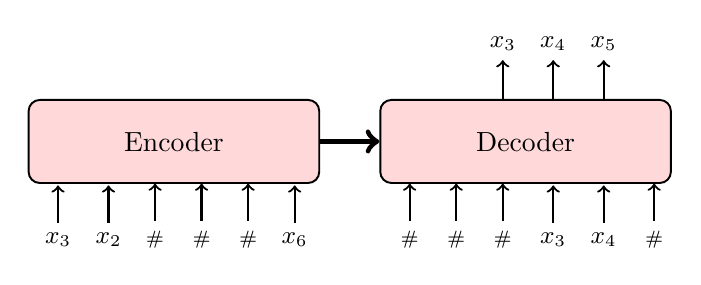
\begin{tikzpicture}
\begin{scope}
\tikzstyle{word} = [font=\scriptsize]
\tikzstyle{model} = [rectangle,draw,minimum height=3em,minimum width=6em,rounded corners=4pt,fill=red!15!white]

\node [anchor=center] (ate) at (0,0) {};

\node [model,minimum width=10.5em,line width=0.7pt] (decoder) at ([xshift=6em]ate.east) {Decoder};
\node [word] (w1) at ([yshift=-2em,xshift=1em]decoder.south) {\small{$x_3$}};
\node [word] (w2) at ([xshift=-1em]w1.west) {\#};
\node [word] (w3) at ([xshift=-1em]w2.west) {\#};
\node [word] (w4) at ([xshift=-1em]w3.west) {\#};
\node [word] (w5) at ([xshift=1em]w1.east) {\small{$x_4$}};
\node [word] (w6) at ([xshift=1em]w5.east) {\#};

\node [word] (w7) at ([yshift=2em,xshift=1em]decoder.north) {\small{$x_4$}};
\node [word] (w8) at ([yshift=0em,xshift=-1em]w7.west) {\small{$x_3$}};
\node [word] (w9) at ([yshift=0em,xshift=1em]w7.east) {\small{$x_5$}};

\draw [->,thick] (w1.north) -- ([yshift=1.35em]w1.north);
\draw [->,thick] (w2.north) -- ([yshift=1.35em]w2.north);
\draw [->,thick] (w3.north) -- ([yshift=1.35em]w3.north);
\draw [->,thick] (w4.north) -- ([yshift=1.35em]w4.north);
\draw [->,thick] (w5.north) -- ([yshift=1.35em]w5.north);
\draw [->,thick] (w6.north) -- ([yshift=1.35em]w6.north);

\draw [->,thick] ([yshift=-1.4em]w7.south) -- (w7.south);
\draw [->,thick] ([yshift=-1.4em]w8.south) -- (w8.south);
\draw [->,thick] ([yshift=-1.4em]w9.south) -- (w9.south);

%encoder
\node [model,minimum width=10.5em,line width=0.7pt] (encoder) at ([xshift=-6em]ate.west) {Encoder};
\node [word] (we1) at ([yshift=-2em,xshift=1em]encoder.south) {\#};
\node [word] (we2) at ([xshift=-1em]we1.west) {\#};
\node [word] (we3) at ([xshift=-1em]we2.west) {\small{$x_2$}};
\node [word] (we4) at ([xshift=-1em]we3.west) {\small{$x_3$}};
\node [word] (we5) at ([xshift=1em]we1.east) {\#};
\node [word] (we6) at ([xshift=1em]we5.east) {\small{$x_6$}};

\draw [->,thick] (we1.north) -- ([yshift=1.35em]we1.north);
\draw [->,thick] (we2.north) -- ([yshift=1.35em]we2.north);
\draw [->,thick] (we3.north) -- ([yshift=1.35em]we3.north);
\draw [->,thick] (we4.north) -- ([yshift=1.35em]we4.north);
\draw [->,thick] (we5.north) -- ([yshift=1.35em]we5.north);
\draw [->,thick] (we6.north) -- ([yshift=1.35em]we6.north);

\draw [->,line width=2pt] ([xshift=0.5em]encoder)--([xshift=-0.5em]decoder);
\end{scope}
\end{tikzpicture}
\caption{MASS 预训练方法}
\label{fig:16-6}
\end{figure}
%----------------------------------------------

\parinterval  此外,还有很多问题值得探讨。例如,为何预训练词嵌入在神经机器翻译模型中有效\upcite{2018When};如何在神经机器翻译模型中利用预训练的BERT模型\upcite{DBLP:conf/emnlp/ClinchantJN19,DBLP:conf/emnlp/ImamuraS19,DBLP:conf/aaai/YangW0Z00020,DBLP:conf/aaai/WengYHCL20,DBLP:conf/emnlp/ImamuraS19};如何针对神经机器翻译任务进行预训练\upcite{DBLP:journals/corr/abs-2001-08210,DBLP:conf/aaai/JiZDZCL20,DBLP:conf/acl/LewisLGGMLSZ20};如何针对机器翻译中的Code-switching问题进行预训练\upcite{DBLP:journals/corr/abs-2009-08088};如何在微调过程中避免灾难性遗忘\upcite{DBLP:journals/corr/abs-2010-09403}。

%----------------------------------------------------------------------------------------
%    NEW SUB-SUB-SECTION
%----------------------------------------------------------------------------------------
\subsubsection{4. 多任务学习}

\parinterval 在训练一个神经网络的时候,如果过分地关注单个训练目标,可能使模型忽略掉其他可能有帮助的信息,这些信息可能来自于一些其他相关的任务\upcite{DBLP:journals/corr/Ruder17a}。通过联合多个独立但相关的任务共同学习,任务之间相互``促进'',就是多任务学习\upcite{DBLP:journals/corr/Ruder17a,DBLP:books/sp/98/Caruana98,liu2019multi}。多任务学习的常用做法是,针对多个相关的任务,共享模型的部分参数来学习不同任务之间相似的特征,并通过特定的模块来学习每个任务独立的特征(见\chapterfifteen)。常用的策略是对底层的模型参数进行共享,顶层的模型参数用于独立学习各个不同的任务。

%----------------------------------------------
\begin{figure}[htp]
    \centering
    
%%% outline
%-------------------------------------------------------------------------
\begin{tikzpicture}
\tikzstyle{rec} = [line width=0.6pt,draw,rounded corners,minimum height=2.2em,minimum width=4.3em]



\node [anchor=center] (node1-1) at (0,0) {\small{$y$}};
\node[anchor=north,rec,fill=blue!20](node1-2) at ([yshift=-2.0em]node1-1.south) {\small{解码器}};
\node[anchor=north,rec,fill=red!20](node1-3) at ([yshift=-2em]node1-2.south) {\small{编码器}};
\node[anchor=east](node1-5) at ([xshift=-2em]node1-2.west) {\small{$y_{<}$}};
\node[anchor=north](node1-4) at ([yshift=-2em]node1-3.south) {\small{$x$}};
\draw [->,thick](node1-4.north)--(node1-3.south);
\draw [->,thick](node1-5.east)--(node1-2.west);
\draw [->,thick](node1-3.north)--(node1-2.south);
\draw [->,thick](node1-2.north)--(node1-1.south);

\node [anchor=center] (node2-1) at ([xshift=12.0em]node1-1.east) {\small{$y$}};
\node[anchor=north,rec,fill=blue!20](node2-2) at ([yshift=-2.0em]node2-1.south) {\small{解码器}};
\node[anchor=north,rec,fill=red!20](node2-3) at ([yshift=-2em]node2-2.south) {\small{编码器}};
\node[anchor=east](node2-5) at ([xshift=-2em]node2-2.west) {\small{$y_{<}$}};
\node[anchor=north](node2-4) at ([yshift=-2em]node2-3.south) {\small{$x$}};
\node[anchor=west,rec,fill=yellow!20](node2-6) at ([xshift=3.0em]node2-3.east) {\small{解码器}};
\node[anchor=south](node2-7) at ([yshift=2em]node2-6.north) {\small{$\hat{x}$}};

\draw [->,thick](node2-4.north)--(node2-3.south);
\draw [->,thick](node2-5.east)--(node2-2.west);
\draw [->,thick](node2-3.north)--(node2-2.south);
\draw [->,thick](node2-2.north)--(node2-1.south)node[pos=0.5,left,font=\scriptsize]{翻译};
\draw [->,thick](node2-3.east)--(node2-6.west);
\draw [->,thick](node2-6.north)--(node2-7.south)node[pos=0.5,left,font=\scriptsize]{调整语序};

\node [anchor=east] (node1) at ([xshift=-2.0em]node1-1.west) {\small{$x,y$:双语数据}};
\node [anchor=south] (node2) at ([xshift=1.96em]node1.north) {\small{$y_{<}$:目标语言文本数据}};

\node [anchor=north](pos1) at ([yshift=0em]node1-4.south) {\small{(a)单任务学习}};
\node [anchor=west](pos2) at ([xshift=10.0em]pos1.east) {\small{(b)多任务学习}};

\end{tikzpicture}
    \caption{使用源语言单语数据的多任务学习}
    \label{fig:16-7}
\end{figure}
%----------------------------------------------

\parinterval 在神经机器翻译中,应用多任务学习的主要策略是将翻译任务作为主任务,同时设置一些仅使用单语数据的子任务,通过这些子任务来捕捉单语数据中的语言知识\upcite{DBLP:conf/emnlp/DomhanH17,DBLP:conf/emnlp/ZhangZ16,DBLP:journals/corr/LuongLSVK15}。一种多任务学习的方法是利用源语言单语数据,通过单个编码器对源语言数据进行建模,再分别使用两个解码器来学习源语言排序和翻译任务。源语言排序任务是指利用预排序规则对源语言句子中词的顺序进行调整\upcite{DBLP:conf/emnlp/WangCK07},可以通过单语数据来构造训练数据,从而使编码器被训练得更加充分\upcite{DBLP:conf/emnlp/ZhangZ16},如图\ref{fig:16-7}所示,图中$y_{<}$表示当前时刻之前的单词序列,$x_{<}$表示源语言句子中词的顺序调整后的句子。

\parinterval 虽然神经机器翻译模型可以看作一种语言生成模型,但生成过程中却依赖于源语言信息,因此无法直接利用目标语言单语数据进行多任务学习。针对这个问题,可以对原有翻译模型结构进行修改,在解码器底层增加一个语言模型子层,这个子层用于学习语言模型任务,与编码器端是完全独立的,如图\ref{fig:16-8}所示\upcite{DBLP:conf/emnlp/DomhanH17},图中$y_{<}$表示当前时刻之前的单词序列,$z_{<}$表示当前时刻之前的单语数据。在训练过程中,分别将双语数据和单语数据送入翻译模型和语言模型进行计算,双语数据训练产生的梯度用于对整个模型进行参数更新,而单语数据产生的梯度只对语言模型子层进行参数更新。

%----------------------------------------------
\begin{figure}[htp]
\centering
\begin{tikzpicture}

\tikzstyle{rec} = [line width=0.6pt,draw,rounded corners,minimum height=2.2em,minimum width=4.3em]



\node [anchor=center] (node1-1) at (0,0) {\small{$y$}};
\node[anchor=north,rec,fill=blue!20](node1-2) at ([yshift=-2.0em]node1-1.south) {\small{解码器}};
\node[anchor=north,rec,fill=red!20](node1-3) at ([yshift=-2em]node1-2.south) {\small{编码器}};
\node[anchor=east](node1-5) at ([xshift=-2em]node1-2.west) {\small{$y_{<}$}};
\node[anchor=north](node1-4) at ([yshift=-2em]node1-3.south) {\small{$x$}};
\draw [->,thick](node1-4.north)--(node1-3.south);
\draw [->,thick](node1-5.east)--(node1-2.west);
\draw [->,thick](node1-3.north)--(node1-2.south);
\draw [->,thick](node1-2.north)--(node1-1.south);


\node [anchor=center] (node2-1) at ([xshift=10.0em,yshift=-7.43em]node1-1.east) {\small{$x$}};
\node[anchor=south,rec,fill=blue!20](node2-2) at ([yshift=2.0em]node2-1.north) {\small{编码器}};
\node[anchor=west,rec,fill=red!20](node2-3) at ([xshift=2em]node2-2.east) {\small{解码器}};

\node[anchor=south](node2-4) at ([yshift=2em]node2-3.north) {\small{$y$}};
\node[anchor=north,rec,fill=yellow!20](node2-5) at ([yshift=-2.0em]node2-3.south) {\small{语言模型}};
\node[anchor=north](node2-6) at ([yshift=-2em]node2-5.south) {\small{$y_{<}+z_{<}$}};
\node[anchor=west](node2-7) at ([xshift=2em]node2-5.east) {\small{z}};
\node [rectangle,rounded corners,draw=red,line width=0.2mm,densely dashed,inner sep=0.4em] [fit = (node2-5) (node2-7)] (inputshadow) {};


\draw [->,thick](node2-1.north)--(node2-2.south);
\draw [->,thick](node2-2.east)--(node2-3.west);
\draw [->,thick](node2-3.north)--(node2-4.south);
\draw [->,thick](node2-5.north)--(node2-3.south);
\draw [->,thick](node2-6.north)--(node2-5.south);
\draw [->,thick](node2-5.east)--(node2-7.west);

\node [anchor=east] (node1) at ([yshift=1.6em,xshift=-2.0em]node1-1.west) {\small{$x,y$:双语数据}};
\node [anchor=south] (node2) at ([xshift=1.96em]node1.north) {\small{$y_{<}$:目标语言文本数据}};
\node [anchor=north] (node3) at ([xshift=0.45em]node1.south) {\small{$z$}:单语数据};

\node [anchor=north](pos1) at ([yshift=0em]node1-4.south) {\small{(a)单任务学习}};
\node [anchor=west](pos2) at ([xshift=10.0em]pos1.east) {\small{(b)多任务学习}};


\end{tikzpicture}
\caption{使用语言模型的多任务学习}
\label{fig:16-8}
\end{figure}
%----------------------------------------------

\parinterval 此外,一种策略是利用多任务学习的思想来训练多到一模型(多个编码器、单个解码器)、一到多模型(单个编码器、多个解码器)和多到多模型(多个编码器、多个解码器),从而借助单语数据或其他数据来使编码器或解码器训练得更加充分\upcite{DBLP:journals/corr/LuongLSVK15},任务的形式包括翻译任务、句法分析任务、图像分类等。另外一种策略是利用多任务学习的思想同时训练多个语言的翻译任务\upcite{DBLP:conf/acl/DongWHYW15,DBLP:journals/tacl/JohnsonSLKWCTVW17},同样包括多到一翻译(多个语种到一个语种)、一到多翻译(一个语种到多个语种)以及多到多翻译(多个语种到多个语种),这种方法可以利用多种语言的训练数据进行学习,具有较大的潜力,逐渐受到了研究人员们的关注,具体内容可以参考\ref{multilingual-translation-model}节。

%----------------------------------------------------------------------------------------
%    NEW SECTION 16.2
%----------------------------------------------------------------------------------------
\sectionnewpage
\section{双向翻译模型}

\parinterval 在机器翻译任务中,对于给定的双语数据,可以同时学习源语言到目标语言和目标语言到源语言的翻译模型,因此机器翻译可被视为一种双向任务。那么,两个方向的翻译模型能否联合起来,相辅相成呢?下面将从双向训练和对偶学习两方面对双向翻译模型进行介绍。这些方法被大量使用在低资源翻译系统中,比如,可以用双向翻译模型反复迭代构造伪数据。

%----------------------------------------------------------------------------------------
%    NEW SUB-SUB-SECTION
%----------------------------------------------------------------------------------------
\subsection{双向训练}

\parinterval 回顾神经机器翻译系统的建模过程,给定一个互译的句对$(\seq{x},\seq{y})$,一个从源语言句子$\seq{x}$到目标语言句子$\seq{y}$的翻译被表示为求条件概率$\funp{P}(\seq{y}|\seq{x})$的问题。类似地,一个从目标语言句子$\seq{y}$到源语言句子$\seq{x}$的翻译可以表示为$\funp{P}(\seq{x}|\seq{y})$。通常来说,神经机器翻译的训练一次只得到一个方向的模型,也就是$\funp{P}(\seq{y}|\seq{x})$或者$\funp{P}(\seq{x}|\seq{y})$。这意味着$\funp{P}(\seq{y}|\seq{x})$和$\funp{P}(\seq{x}|\seq{y})$之间是互相独立的。但$\funp{P}(\seq{y}|\seq{x})$和$\funp{P}(\seq{x}|\seq{y})$是否真的没有关系呢?这里以最简单的情况为例,假设$\seq{x}$和$\seq{y}$被表示为相同大小的两个向量$\mathbi{E}_x$和$\mathbi{E}_y$,且$\mathbi{E}_x$到$\mathbi{E}_y$的变换是一个线性变换,也就是与一个方阵$\mathbi{W}$ 做矩阵乘法:
\begin{eqnarray}
\mathbi{E}_y & = & \mathbi{E}_x \cdot \mathbi{W}
\label{eq:16-2}
\end{eqnarray}

\noindent 这里,$\mathbi{W}$应当是一个满秩矩阵,否则对于任意一个$\mathbi{E}_x$经过$\mathbi{W}$变换得到的$\mathbi{E}_y$只落在所有可能的$\mathbi{E}_y$的一个子空间内,即在给定$\mathbi{W}$ 的情况下有些$\seq{y}$ 不能被任何一个$\seq{x}$表达,而这不符合常识,因为不管是什么句子,总能找到它的一种译文。若$\mathbi{W}$是满秩矩阵说明$\mathbi{W}$可逆,也就是给定$\mathbi{E}_x$到$\mathbi{E}_y$ 的变换$\mathbi{W}$ 下,$\mathbi{E}_y$到$\mathbi{E}_x$ 的变换必然是$\mathbi{W}$的逆而不是其他矩阵。

\parinterval 这个例子说明$\funp{P}(\seq{y}|\seq{x})$和$\funp{P}(\seq{x}|\seq{y})$直觉上应当存在联系。当然,$\seq{x}$和$\seq{y}$之间是否存在简单的线性变换关系并没有结论,但是上面的例子给出了一种对源语言句子和目标语言句子进行相互转化的思路。实际上,研究人员已经通过一些数学技巧用目标函数把$\funp{P}(\seq{y}|\seq{x})$和$\funp{P}(\seq{x}|\seq{y})$联系起来,这样训练神经机器翻译系统一次就可以同时得到两个方向的翻译模型,使得训练变得更加高效\upcite{Hassan2018AchievingHP,DBLP:conf/aaai/Zhang0LZC18,DBLP:conf/wmt/SunJXHWW19}。双向联合训练的基本思想是:使用两个方向的翻译模型对单语数据进行推断,之后把翻译结果与原始的单语数据作为训练语料,通过多次迭代更新两个方向上的机器翻译模型。

\parinterval 图\ref{fig:16-9}给出了一个双向训练的流程,其中$M_{x \rightarrow y}^{k}$表示第$k$轮得到的$x$到$y$的翻译模型,$M_{y \rightarrow x}^{k}$表示第$k$轮得到的$y$到$x$的翻译模型。这里只展示了前两轮迭代。在第一次迭代开始之前,首先使用双语数据对两个初始翻译模型进行训练。为了保持一致性,这里称之为第0 轮迭代。在第一轮迭代中,首先使用这两个翻译模型$M_{x \rightarrow y}^{0}$ 和$M_{y \rightarrow x}^{0}$ 翻译单语数据$X=\{ x_i \}$ 和$Y= \{ y_i \}$ 后得到译文$\{\hat{y}_i^{0} \}$和$\{ \hat{x}_i^{0}\}$。进一步,构建伪训练数据集$\{ x_i,\hat{y}_i^{0}\}$ 与$\{ \hat{x}_i^{0},y_i \}$。然后使用上面的两个伪训练数据集和原始双语数据混合,训练得到模型$M_{x \rightarrow y}^{1}$和$M_{y \rightarrow x}^{1}$并进行参数更新,即用$\{ \hat{x}_i^{0},y_i\} \bigcup \{ x_i,y_i\}$训练$M_{x \rightarrow y}^{1}$,用$\{ \hat{y}_i^{0},x_i\} \bigcup \{ y_i,x_i\}$训练$M_{y \rightarrow x}^{1}$。第二轮迭代继续重复上述过程,使用更新参数后的翻译模型$M_{x \rightarrow y}^{1}$和$M_{y \rightarrow x}^{1}$ 得到新的伪数据集$\{ x_i,\hat{y}_i^{1}\}$ 与$\{ \hat{x}_i^{1},y_i \}$。然后,进一步得到翻译模型$M_{x \rightarrow y}^{2}$和$M_{y \rightarrow x}^{2}$。这种方式本质上也是一种自学习的过程,逐步生成更好的伪数据,同时提升模型质量。

%----------------------------------------------
\begin{figure}[h]
\centering
\definecolor{color1}{rgb}{1,0.725,0.058}
\tikzstyle{data} = [rectangle,very thick,rounded corners,minimum width=2.3cm,minimum height=0.83cm,text centered,draw=black!70,fill=color1!25]
\tikzstyle{data_shadow} = [rectangle,very thick,rounded corners,minimum width=2.3cm,minimum height=0.83cm,text centered,draw=black!70,fill=black!70]
\tikzstyle{process} = [rectangle,thick,rounded corners,minimum width=2cm,minimum height=0.7cm,text centered,draw=black!80,fill=gray!25]
\tikzstyle{state} = [rectangle,thick,rounded corners,minimum width=3cm,minimum height=0.7cm,text centered,draw=black!80,fill=gray!25]
\begin{tikzpicture}[node distance = 0,scale = 1]
\tikzstyle{every node}=[scale=1]
\node(monolingual_X_shadow)[data_shadow]{};
\node(bilingual_D_shadow)[data_shadow, right of = monolingual_X_shadow, xshift=5cm]{};
\node(monolingual_Y_shadow)[data_shadow, right of = bilingual_D_shadow, xshift=5cm]{};
\node(monolingual_X)[data,right of = monolingual_X_shadow,xshift=-0.08cm,yshift=0.08cm]{单语语料X};
\node(bilingual_D)[data, right of = monolingual_X, xshift=5cm, fill=ugreen!30]{双语语料D};
\node(monolingual_Y)[data, right of = bilingual_D, xshift=5cm, fill=blue!25]{单语语料Y};

\node(process_1_1)[process, right of = monolingual_X, xshift=2.5cm, yshift=-1.5cm]{\textbf{$M^0_{x\to y}$}};
\node(process_1_2)[process, right of = process_1_1, xshift=5cm, fill=red!25]{$M^0_{y\to x}$};
\node(process_2_1)[process, below of = process_1_1, yshift=-1.2cm]{翻译过程};
\node(process_2_2)[process, below of = process_1_2, yshift=-1.2cm, fill=red!25]{翻译过程};
\node(process_3_1)[state, below of = process_2_1, yshift=-1.2cm, fill=color1!25]{\{$x_i,\hat{y}^0_i$\}};
\node(process_3_2)[state, below of = process_2_2, yshift=-1.2cm, fill=blue!25]{\{$\hat{x}^0_i,{y_i}$\}};
\node(process_4_1)[process, below of = process_3_1, yshift=-1.2cm]{\textbf{$M^1_{x\to y}$}};
\node(process_4_2)[process, below of = process_3_2, yshift=-1.2cm, fill=red!25]{$M^1_{y\to x}$};
\node(process_5_1)[process, below of = process_4_1, yshift=-1.2cm]{翻译过程};
\node(process_5_2)[process, below of = process_4_2, yshift=-1.2cm, fill=red!25]{翻译过程};
\node(process_6_1)[state, below of = process_5_1, yshift=-1.2cm, fill=color1!25]{\{$x_i,\hat{y}^1_i$\}};
\node(process_6_2)[state, below of = process_5_2, yshift=-1.2cm, fill=blue!25]{\{$\hat{x}^1_i,{y_i}$\}};
\node(process_7_1)[process, below of = process_6_1, yshift=-1.2cm]{\textbf{$M^2_{x\to y}$}};
\node(process_7_2)[process, below of = process_6_2, yshift=-1.2cm, fill=red!25]{$M^2_{y\to x}$};
\node(ellipsis_1)[below of = monolingual_X, yshift=-9.9cm,scale=1.5]{$...$};
\node(ellipsis_2)[below of = process_7_1, yshift=-1.2cm,scale=1.5]{$...$};
\node(ellipsis_3)[below of = bilingual_D, yshift=-9.9cm,scale=1.5]{$...$};
\node(ellipsis_4)[below of = process_7_2, yshift=-1.2cm,scale=1.5]{$...$};
\node(ellipsis_5)[below of = monolingual_Y, yshift=-9.9cm,scale=1.5]{$...$};
\node(text_1)[left of = process_2_1, xshift=-4cm,scale=0.8]{第0轮迭代};
\node(text_2)[left of = process_5_1, xshift=-4cm,scale=0.8]{第1轮迭代};
\node(text_3)[left of = ellipsis_2, xshift=-4cm, scale=0.8]{第2轮迭代};
\draw[->, very thick, color=color1!40](monolingual_X.south)--(ellipsis_1.north);
\draw[->, very thick, color=ugreen!30](bilingual_D.south)--(ellipsis_3.north);
\draw[->, very thick, color=blue!55](monolingual_Y.south)--(ellipsis_5.north);
\draw[->, very thick, color=color1!40]([xshift=-1.5cm]process_2_1.west)--(process_2_1.west);
\draw[->, very thick, color=color1!40]([xshift=-1.5cm]process_5_1.west)--(process_5_1.west);
\draw[->, very thick, color=blue!55]([xshift=1.5cm]process_2_2.east)--(process_2_2.east);
\draw[->, very thick, color=blue!55]([xshift=1.5cm]process_5_2.east)--(process_5_2.east);
\draw[->, thick](process_1_1.south)--(process_2_1.north);
\draw[->, thick](process_1_2.south)--(process_2_2.north);
\draw[->, thick](process_2_1.south)--(process_3_1.north);
\draw[->, thick](process_2_2.south)--(process_3_2.north);
\draw[->, thick](process_4_1.south)--(process_5_1.north);
\draw[->, thick](process_4_2.south)--(process_5_2.north);
\draw[->, thick](process_5_1.south)--(process_6_1.north);
\draw[->, thick](process_5_2.south)--(process_6_2.north);
\draw[->, thick](process_7_1.south)--(ellipsis_2.north);
\draw[->, thick](process_7_2.south)--(ellipsis_4.north);
\draw[->, very thick, color=color1!40](process_3_1.east)--([yshift=0.35cm]process_4_2.west);
\draw[->, very thick, color=color1!40](process_3_2.west)--([yshift=0.35cm]process_4_1.east);
\draw[->, very thick, color=color1!40](process_6_1.east)--([yshift=0.35cm]process_7_2.west);
\draw[->, very thick, color=color1!40](process_6_2.west)--([yshift=0.35cm]process_7_1.east);
\draw[->, very thick, color=ugreen!30,in=0,out=270]([xshift=-0.3cm]bilingual_D.south)to(process_1_1.east);
\draw[->, very thick, color=ugreen!30,in=180,out=270]([xshift=0.3cm]bilingual_D.south)to(process_1_2.west);
\draw[->, very thick, color=ugreen!30,in=0,out=270]([yshift=-3.7cm]bilingual_D.south)to(process_4_1.east);
\draw[->, very thick, color=ugreen!30,in=180,out=270]([yshift=-3.7cm]bilingual_D.south)to(process_4_2.west);
\draw[->, very thick, color=ugreen!30,in=0,out=270]([yshift=-7.3cm]bilingual_D.south)to(process_7_1.east);
\draw[->, very thick, color=ugreen!30,in=180,out=270]([yshift=-7.3cm]bilingual_D.south)to(process_7_2.west);
\draw[->, very thick, color=ugreen!30,in=180,out=270]([yshift=-7.3cm]bilingual_D.south)to(process_7_2.west);

\draw[-, very thick, dashed, color=blue!55]([xshift=-1cm,yshift=-0.35cm]text_1.south)--([xshift=12.7cm,yshift=-0.35cm]text_1.south);
\draw[-, very thick, dashed, color=blue!55]([xshift=-1cm,yshift=-0.35cm]text_2.south)--([xshift=12.7cm,yshift=-0.35cm]text_2.south);
\draw[-, very thick, dashed, color=blue!55]([xshift=-1cm,yshift=-0.35cm]text_3.south)--([xshift=12.7cm,yshift=-0.35cm]text_3.south);
\end{tikzpicture}
\caption{翻译模型的双向训练}
\label{fig:16-9}
\end{figure}
%----------------------------------------------
%----------------------------------------------------------------------------------------
%    NEW SUB-SECTION
%----------------------------------------------------------------------------------------
\subsection{对偶学习}

\parinterval 对称,也许是人类最喜欢的美,其始终贯穿在整个人类文明的诞生与发展之中。古语“夫美者,上下、内外、大小、远近皆无害焉,故曰美”描述的即是这样的美。在人工智能的任务中,也存在着这样的对称结构,比如机器翻译中英译汉和汉译英、图像处理中的图像标注和图像生成,以及语音处理中的语音识别和语音合成等。利用这些任务的对称性质(也称对偶性),可以使互为对偶的两个任务获得更有效的反馈,从而使对应的模型相互学习、相互提高。



目前,对偶学习的思想已经广泛应用于低资源机器翻译领域,它不仅能够提升在有限双语资源下的翻译模型性能,而且能够利用未标注的单语数据来进行学习。下面将针对{\small\bfnew{有监督对偶学习}}\index{有监督对偶学习}(Dual Supervised Learning\index{Dual Supervised Learning})\upcite{DBLP:conf/icml/XiaQCBYL17,DBLP:conf/icml/XiaTTQYL18}与{\small\bfnew{无监督对偶学习}}\index{无监督对偶学习}(Dual Unsupervised Learning\index{Dual Unsupervised Learning})\upcite{qin2020dual,DBLP:conf/nips/HeXQWYLM16,zhao2020dual}两方面,对对偶学习的思想进行介绍。

%----------------------------------------------------------------------------------------
%    NEW SUB-SUB-SECTION
%----------------------------------------------------------------------------------------
\subsubsection{1. 有监督对偶学习}

\parinterval 对偶学习涉及两个任务,分别是原始任务和它的对偶任务。在机器翻译任务中,给定一个互译的句对$(\seq{x},\seq{y})$,原始任务学习一个条件概率$\funp{P}(\seq{y}|\seq{x})$将源语言句子$\seq{x}$翻译成目标语言句子$\seq{y}$;对偶任务同样学习一个条件概率$\funp{P}(\seq{x}|\seq{y})$将目标语言句子$\seq{y}$翻译成源语言句子$\seq{x}$。除了使用条件概率建模翻译问题,还可以使用联合分布$\funp{P}(\seq{x},\seq{y})$进行建模。根据条件概率定义,有:
\begin{eqnarray}
\funp{P}(\seq{x},\seq{y}) &=& \funp{P}(\seq{x})\funp{P}(\seq{y}|\seq{x}) \nonumber \\
&=& \funp{P}(\seq{y})\funp{P}(\seq{x}|\seq{y})
\label{eq:16-3}
\end{eqnarray}

\parinterval 公式\eqref{eq:16-3}很自然地把两个方向的翻译模型$\funp{P}(\seq{y}|\seq{x})$和$\funp{P}(\seq{x}|\seq{y})$以及两个语言模型$\funp{P}(\seq{x})$和$\funp{P}(\seq{y})$联系起来:$\funp{P}(\seq{x})\funp{P}(\seq{y}|\seq{x})$应该与$\funp{P}(\seq{y})\funp{P}(\seq{x}|\seq{y})$接近,因为它们都表达了同一个联合分布$\funp{P}(\seq{x},\seq{y})$。因此,在构建训练两个方向的翻译模型的目标函数时,除了它们单独训练时各自使用的极大似然估计目标函数,可以额外增加一个目标项来鼓励两个方向的翻译模型,例如:
\begin{eqnarray}
{L}_{\rm{dual}} & = & \Big(\log{\funp{P}(\seq{x})} + \log{\funp{P}(\seq{y}|\seq{x})} - \log{\funp{P}(\seq{y})} - \log{\funp{P}(\seq{x}|\seq{y})\Big)^{2}}
\label{eq:16-4}
\end{eqnarray}

\parinterval 通过该正则化项,互为对偶的两个任务可以被放在一起学习,通过任务对偶性加强监督学习的过程,就是有监督对偶学习\upcite{DBLP:conf/icml/XiaQCBYL17,qin2020dual}。这里,$\funp{P}(\seq{x})$和$\funp{P}(\seq{y})$两个语言模型是预先训练好的,并不参与翻译模型的训练。可以看到,对于单独的一个模型来说,其目标函数增加了与另外一个方向的模型相关的损失项。这样的形式与L1/L2正则化非常类似(见{\chapterthirteen}),因此可以把这个方法看作是一种正则化的手段(由翻译任务本身的性质所启发而来)。有监督对偶学习实际上要优化如下的损失函数:
\begin{eqnarray}
{L} & = &  \log{\funp{P}(\seq{y}|\seq{x})}+\log{\funp{P}(\seq{x}|\seq{y})}+{L}_{\rm{dual}}
\label{eq:16-5}
\end{eqnarray}

\parinterval 由于两个方向的翻译模型和语言模型相互影响,这种共同训练、共同提高的方法能得到比基于单个方向训练效果更好的模型。

%----------------------------------------------------------------------------------------
%    NEW SUB-SUB-SECTION
%----------------------------------------------------------------------------------------
\subsubsection{2. 无监督对偶学习}

\parinterval 有监督的对偶学习需要使用双语数据来训练两个翻译模型,但是有些低资源语言仅有少量双语数据可以训练。因此,如何使用资源相对丰富的单语数据来提升翻译模型的性能也是一个关键问题。

\parinterval 无监督对偶学习提供了一个解决问题的思路\upcite{qin2020dual}。假设目前有两个比较弱的翻译模型,一个原始翻译模型$f$将源语言句子$\seq{x}$翻译成目标语言句子$\seq{y}$,一个对偶任务模型$g$将目标语言句子$\seq{y}$翻译成源语言句子$\seq{x}$。翻译模型可由有限的双语训练,或者使用无监督机器翻译得到(见\ref{sec:unsupervised-nmt}节)。如图\ref{fig:16-10}所示,无监督对偶学习的做法是,先通过原始任务模型$f$ 将一个源语言单语句子$x$翻译为目标语言句子$y$,随后,再通过对偶任务模型$g$将目标语言句子$y$翻译为源语言句子$x^{'}$。如果模型$f$和$g$的翻译性能较好,那么$x^{'}$和$x$会十分相似。通过计算二者的{\small\bfnew{重构损失}}\index{重构损失}(Reconstruction Loss)\index{Reconstruction Loss},就可以优化模型$f$和$g$的参数。这个过程可以多次迭代,从大量的无标注单语数据上不断提升性能。

%----------------------------------------------
\begin{figure}[htp]
\centering
\begin{tikzpicture}

\tikzstyle{circle} = [draw,black,line width=0.6pt,inner sep=3.5pt,rounded corners=4pt,minimum width=2em]
\tikzstyle{word} = [inner sep=3.5pt]

\node [anchor=center] (node1-1) at (0,0) {\small{$\seq{x}$}};
\node [anchor=west] (node1-2) at ([xshift=0.8em]node1-1.east) {\small{$\seq{y}$}};
\node [anchor=north] (node1-3) at ([xshift=1.0em]node1-1.south) {\small{翻译模型$f$}};
\draw [->,line width=0.6pt](node1-1.east)--(node1-2.west);

\begin{pgfonlayer}{background}
{
\node[fill=blue!20,inner sep=0.1em,draw=black,line width=0.6pt,minimum width=5em,drop shadow,rounded corners=2pt] [fit =(node1-1)(node1-2)(node1-3)]  (remark1) {};
}
\end{pgfonlayer}

\node[anchor=north,circle,fill=red!20,minimum width=6.8em](node2) at ([xshift=-6.0em,yshift=-2.0em]remark1.south) {源语言句子$\seq{x}$};
\node[anchor=north,circle,fill=red!20,minimum width=6.8em](node2-2) at ([yshift=-0.2em]node2.south) {新生成句子$\seq{x'}$};
\draw [->,thick]([yshift=0.2em]node2.north).. controls (-1.93,-1.5) and (-2.0,-0.2)..([xshift=-0.2em]remark1.west);
\node[anchor=north,circle,fill=red!20](node3) at ([xshift=6.5em,yshift=-2.0em]remark1.south) {目标语言句子$\seq{y}$};
\draw [->,thick]([xshift=0.2em]remark1.east).. controls (2.9,-0.25) and (2.9,-0.7) ..([yshift=0.2em]node3.north);


\node [anchor=north] (node4-1) at ([xshift=-1.0em,yshift=-7.0em]remark1.south) {\small{$\seq{y}$}};
\node [anchor=west] (node4-2) at ([xshift=0.8em]node4-1.east) {\small{$\seq{x}$}};
\node [anchor=north] (node4-3) at ([xshift=1.0em]node4-1.south) {\small{翻译模型$g$}};
\draw [->,line width=0.6pt](node4-1.east)--(node4-2.west);

\begin{pgfonlayer}{background}
{
\node[fill=yellow!20,inner sep=0.1em,draw=black,line width=0.6pt,minimum width=5em,drop shadow,rounded corners=2pt] [fit =(node4-1)(node4-2)(node4-3)]  (remark2) {};
}
\end{pgfonlayer}

\draw [->,thick]([xshift=-0.2em]remark2.west).. controls (-0.8,-4.12) and (-1.95,-4.12)..([yshift=-0.2em]node2-2.south);
\draw [->,thick]([yshift=-0.2em]node3.south).. controls (2.9,-3) and (2.9,-4.1)..([xshift=0.2em]remark2.east);

\end{tikzpicture}
\caption{无监督对偶学习流程}
\label{fig:16-10}
\end{figure}
%----------------------------------------------

\parinterval 这个过程与强化学习的流程非常相似(见{\chapterthirteen})。在训练过程中,模型无法知道某个状态下正确的行为是什么,只能通过这种试错-反馈的机制来反复调整。训练这两个模型可以用已有的强化学习算法来训练,比如策略梯度方法\upcite{DBLP:conf/nips/SuttonMSM99}。策略梯度的基本思想如下:如果在执行某个动作之后,获得了一个不错的反馈,那么会调整策略来增加这个状态下执行该动作的概率;反之,如果采取某个动作后获得了一个负反馈,就需要调整策略来降低这个状态下执行该动作的概率。

%----------------------------------------------------------------------------------------
%    NEW SECTION
%----------------------------------------------------------------------------------------
\sectionnewpage
\section{多语言翻译模型}\label{multilingual-translation-model}

\parinterval 低资源机器翻译面临的主要挑战是缺乏大规模高质量的双语数据。这个问题往往伴随着多语言的翻译任务\upcite{dabre2020survey}。也就是,要同时开发多个不同语言之间的机器翻译系统,其中少部分语言是富资源语言,而其它语言是低资源语言。针对低资源语言双语数据稀少或者缺失的情况,一种常见的思路是利用富资源语言的数据或者系统帮助低资源机器翻译系统。这也构成了多语言翻译的思想,并延伸出大量的研究工作,其中有三个典型研究方向:基于枢轴语言的方法\upcite{DBLP:journals/mt/WuW07}、 基于知识蒸馏的方法\upcite{DBLP:journals/corr/ChenLCL17}、基于迁移学习的方法\upcite{DBLP:conf/emnlp/KimPPKN19,DBLP:journals/tacl/JohnsonSLKWCTVW17},下面进行介绍。

%----------------------------------------------------------------------------------------
%    NEW SUB-SECTION
%----------------------------------------------------------------------------------------

\subsection{基于枢轴语言的方法}
\label{sec:pivot-based-translation}

\parinterval 传统的多语言翻译中,广泛使用的是{\small\bfnew{基于枢轴语言的翻译}}(Pivot-based Translation)\upcite{DBLP:conf/emnlp/KimPPKN19,DBLP:journals/mt/WuW07}。这种方法会使用一种数据丰富的语言作为{\small\bfnew{枢轴语言}}\index{枢轴语言}(Pivot Language)\index{Pivot Language}。翻译过程分为两个阶段:源语言到枢轴语言的翻译,枢轴语言到目标语言的翻译。这样,通过资源丰富的枢轴语言将源语言和目标语言桥接在一起,达到解决源语言-目标语言双语数据缺乏的问题。比如,想要得到泰语到波兰语的翻译,可以通过英语做枢轴语言。通过“泰语$\to$英语$\to$波兰语”的翻译过程完成泰语到波兰语的转换。

\parinterval 在统计机器翻译中,有很多基于枢轴语言的方法\upcite{DBLP:conf/naacl/UtiyamaI07,DBLP:conf/acl/ZahabiBK13,DBLP:conf/emnlp/ZhuHWZWZ14,DBLP:conf/acl/MiuraNSTN15},这些方法也已经广泛用于低资源翻译任务\upcite{DBLP:conf/acl/CohnL07,DBLP:journals/mt/WuW07,DBLP:conf/acl/WuW09,de2006catalan}。由于基于枢轴语言的方法与模型结构无关,这些方法也适用于神经机器翻译,并且取得了不错的效果\upcite{DBLP:conf/emnlp/KimPPKN19,DBLP:journals/corr/ChengLYSX16}。

\parinterval 基于枢轴语言的方法可以被描述为如图\ref{fig:16-11}所示的过程。这里,使用虚线表示具有双语平行语料库的语言对,并使用带有箭头的实线表示翻译方向,令$\seq{x}$、$\seq{y}$和$\seq{p}$ 分别表示源语言、目标语言和枢轴语言,对于输入源语言句子$\seq{x}$和目标语言句子$\seq{y}$,其翻译过程可以被建模为:

\begin{eqnarray}
{\funp{P}(\seq{y}|\seq{x})} & = & {\sum_{\seq{p}}{\funp{P}(\seq{p}|\seq{x})\funp{P}(\seq{y}|\seq{p})}}
\label{eq:16-6}
\end{eqnarray}

\noindent 其中,$\seq{p}$表示一个枢轴语言句子。$\funp{P}(\seq{p}|\seq{x})$和$\funp{P}(\seq{y}|\seq{p})$的求解可以直接复用既有的模型和方法。不过,枚举所有的枢轴语言句子$\seq{p}$是不可行的。因此一部分研究工作也探讨了如何选择有效的路径,从$\seq{x}$经过少量$\seq{p}$到达$\seq{y}$\upcite{DBLP:conf/naacl/PaulYSN09}。

%----------------------------------------------
\begin{figure}[h]
\centering

%%% outline
%-------------------------------------------------------------------------
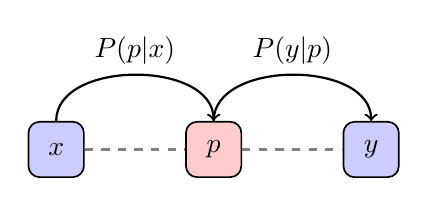
\begin{tikzpicture}

\node[draw,circle,inner sep=2pt,minimum size=2em,fill=blue!20,line width=0.6pt] (x) at (0,0) {$\seq{x}$};

\node[draw,circle,inner sep=2pt,minimum size=2em,fill=red!20,line width=0.6pt] (p) at (2,0) {$\seq{p}$};

\node[draw,circle,inner sep=2pt,minimum size=2em,fill=blue!20,line width=0.6pt] (y) at (4,0) {$\seq{y}$};

\draw[-,dashed,thick,black!50] (x.0) -- (p.180);
\draw[-,dashed,thick,black!50] (p.0) -- (y.180);
\draw[->,out=90,in=90,thick] (x.90) to node[above]{$\funp{P}(\seq{p}|\seq{x})$}(p.90);
\draw[->,out=90,in=90,thick] (p.90) to node[above]{$\funp{P}(\seq{y}|\seq{p})$}(y.90);

\end{tikzpicture}





\caption{基于枢轴语言的翻译过程}
\label{fig:16-11}
\end{figure}
%----------------------------------------------

\parinterval 虽然基于枢轴语言的方法简单且易于实现,但该方法也有一些不足。例如,它需要两次翻译,时间开销较大。而且在两次翻译中,翻译错误会进行累积从而产生错误传播问题,导致模型翻译准确性降低。此外,基于枢轴语言的方法仍然假设源语言和枢轴语言(或者目标语言和枢轴语言)之间存在一定规模的双语平行数据,但是这个假设在很多情况下并不成立。比如,对于一些资源极度稀缺的语言,其到英语或者汉语的双语数据仍然十分匮乏,这时使用基于枢轴语言的方法的效果往往也并不理想。虽然存在以上问题,基于枢轴语言的方法仍然受到工业界的青睐,很多在线翻译引擎也在大量使用这种方法进行多语言的翻译。

%----------------------------------------------------------------------------------------
%    NEW SUB-SECTION
%----------------------------------------------------------------------------------------

\subsection{基于知识蒸馏的方法}

\parinterval 为了缓解基于枢轴语言的方法中存在的错误传播等问题,可以采用基于知识蒸馏的方法\upcite{DBLP:journals/corr/ChenLCL17,DBLP:conf/iclr/TanRHQZL19}。知识蒸馏是一种常用的模型压缩方法\upcite{Hinton2015Distilling},基于教师-学生框架,在第十三章已经进行了详细介绍。针对低资源翻译任务,基于教师-学生框架的方法基本思想如图\ref{fig:16-12}所示。其中,虚线表示具有平行语料库的语言对,带有箭头的实线表示翻译方向。这里,将枢轴语言($\seq{p}$)到目标语言($\seq{y}$)的翻译模型$\funp{P}(\seq{y}|\seq{p})$当作教师模型,源语言($\seq{x}$)到目标语言($\seq{y}$)的翻译模型$\funp{P}(\seq{y}|\seq{x})$当作学生模型。然后,用教师模型来指导学生模型的训练,这个过程中学习的目标就是让$\funp{P}(\seq{y}|\seq{x})$尽可能接近$\funp{P}(\seq{y}|\seq{p})$,这样学生模型就可以学习到源语言到目标语言的翻译知识。举个例子,假设图\ref{fig:16-12}中$\seq{x}$为源语言德语 “hallo”,$\seq{p}$为中间语言英语 “hello”,$\seq{y}$为目标语言法语“bonjour”,则德语“hallo”翻译为法语“bonjour”的概率应该与英语“hello”翻译为法语“bonjour”的概率相近。
%----------------------------------------------
\begin{figure}[h]
\centering

%%% outline
%-------------------------------------------------------------------------
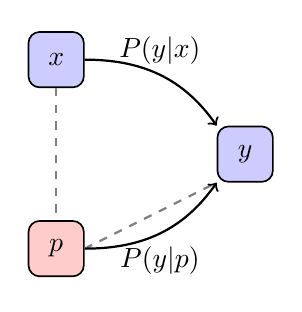
\begin{tikzpicture}

\node[draw,circle,inner sep=2pt,minimum size=2em,fill=blue!20,line width=0.6pt] (x) at (0,0) {$\seq{x}$};

\node[draw,circle,inner sep=2pt,minimum size=2em,fill=red!20,line width=0.6pt] (p) at (0,-2.4) {$\seq{p}$};

\node[draw,circle,inner sep=2pt,minimum size=2em,fill=blue!20,line width=0.6pt] (y) at (2.4,-1.2) {$\seq{y}$};

\draw[-,dashed,thick,black!50] (x.-90) -- (p.90);
\draw[-,dashed,thick,black!50] (p.0) -- (y.-135);
\draw[->,out=0,in=125,thick] (x.0) to node[above]{$\funp{P}(\seq{y}|\seq{x})$}(y.135);
\draw[->,out=0,in=-125,thick] (p.0) to node[below,yshift=-0.1em]{$\funp{P}(\seq{y}|\seq{p})$}(y.-135);

\end{tikzpicture}





\caption{基于教师-学生框架的翻译过程}
\label{fig:16-12}
\end{figure}
%----------------------------------------------

\parinterval 需要注意的是,基于知识蒸馏的方法基于一个假设:如果源语言句子$\seq{x}$、枢轴语言句子$\seq{p}$和目标语言句子$\seq{y}$这三者互译,则$\funp{P}(\seq{y}|\seq{x})$应接近$\funp{P}(\seq{y}|\seq{p})$,即:

\begin{eqnarray}
{\funp{P}(\seq{y}|\seq{x})} & \approx & {\funp{P}(\seq{y}|\seq{p})}
\label{eq:16-7}
\end{eqnarray}

\parinterval 和基于枢轴语言的方法相比,基于知识蒸馏的方法无需训练源语言到枢轴语言的翻译模型,也就无需经历两次翻译过程。不过,基于知识蒸馏的方法仍然需要显性地使用枢轴语言进行桥接,因此仍然面临着“源语言$\to$枢轴语言$\to$目标语言”转换中信息丢失的问题。比如,当枢轴语言到目标语言翻译效果较差时,由于教师模型无法提供准确的指导,学生模型也无法取得很好的学习效果。

%----------------------------------------------------------------------------------------
%    NEW SUB-SECTION
%----------------------------------------------------------------------------------------

\subsection{基于迁移学习的方法}

\parinterval {\small\bfnew{迁移学习}}\index{迁移学习}(Transfer Learning)\index{Transfer Learning}是一种机器学习的方法,指的是一个预训练的模型被重新用在另一个任务中,而并不是从头训练一个新的模型\upcite{Hinton2015Distilling}。迁移学习的目标是将某个领域或任务上学习到的知识应用到新的领域或问题中。在机器翻译中,可以用富资源语言的知识来改进低资源语言上的机器翻译性能,也就是将富资源语言中的知识迁移到低资源语言中。

\parinterval 基于枢轴语言的方法需要显性地建立“源语言$\to$枢轴语言$\to$目标语言”的路径。这时,如果路径中某处出现了问题,就会成为整个路径的瓶颈。如果使用多个枢轴语言,这个问题就会更加严重。不同于基于枢轴语言的方法,迁移学习无需进行两次翻译,也就避免了翻译路径中错误累积的问题。如图\ref{fig:16-13}所示,迁移学习将所有任务分类为源任务和目标任务,目标是将源任务中的知识迁移到目标任务当中。
%----------------------------------------------
\begin{figure}[h]
\centering

%%% outline
%-------------------------------------------------------------------------
\begin{tikzpicture}
	\tikzstyle{node}=[rounded corners=2pt,draw,minimum width=5em,minimum height=2em,drop shadow,font=\footnotesize]

\node[node,fill=blue!20,line width=0.6pt] (nmt1) at (0,0){NMT系统1};
\node[node,anchor=west,fill=yellow!20,line width=0.6pt] (nmt2) at ([xshift=1em]nmt1.east){NMT系统2};
\node[node,anchor=west,fill=red!20,line width=0.6pt] (nmt3) at ([xshift=1em]nmt2.east){NMT系统3};

\node[node,anchor=south,fill=blue!20,line width=0.6pt] (n1) at ([yshift=2.4em]nmt1.north){我不悦};
\node[node,anchor=west,fill=yellow!20,line width=0.6pt] (n2) at ([xshift=1em]n1.east){我不开心};
\node[node,anchor=west,fill=red!20,line width=0.6pt] (n3) at ([xshift=1em]n2.east){吾怀忳忳};

\node[node,anchor=south,fill=green!20,minimum height=1.6em,line width=0.6pt] (task1) at ([yshift=2.6em]n2.north){不同任务};

\node[node,anchor=west,fill=green!20,minimum height=1.6em,line width=0.6pt] (task2) at ([xshift=8em]task1.east){源任务};
\node[node,anchor=north,minimum height=3.2em,fill=orange!20,line width=0.6pt] (n4) at ([yshift=-2em]task2.south){};
\node[draw,anchor=north,cylinder,shape border rotate=90,minimum width=3em,aspect=0.4,fill=orange!20,line width=0.6pt] (kd) at ([yshift=-1.7em]n4.south){\footnotesize 知识};

\node[draw,minimum width=4em,font=\scriptsize,anchor=north,inner ysep=2pt,fill=blue!20,line width=0.6pt] at ([yshift=-2.35em]task2.south){我不悦};
\node[draw,minimum width=4em,font=\scriptsize,anchor=north,inner ysep=2pt,fill=yellow!20,line width=0.6pt] at ([yshift=-3.75em]task2.south){我不开心};

\node[node,anchor=west,fill=green!20,minimum height=1.6em,line width=0.6pt] (task3) at ([xshift=3em]task2.east){目标任务};
\node[node,anchor=north,fill=red!20,line width=0.6pt] (n5) at ([yshift=-2.5em]task3.south){吾怀忳忳};
\node[node,anchor=north,fill=red!20,line width=0.6pt] (sys) at ([yshift=-2.5em]n5.south){学习系统};

\draw[->,thick] ([yshift=-0.2em,xshift=-0.7em]task1.-145) -- node[left,font=\scriptsize,yshift=0.2em]{书面语}([yshift=0.2em]n1.90);
\draw[->,thick] ([yshift=-0.2em]task1.-90) -- node[right,font=\scriptsize,yshift=0.2em,xshift=-0.2em]{口语}([yshift=0.2em]n2.90);
\draw[->,thick] ([yshift=-0.2em,xshift=0.7em]task1.-45) -- node[right,font=\scriptsize,yshift=0.2em]{文言文}([yshift=0.2em]n3.90);
\draw[->,thick] ([yshift=-0.2em]task2.-90) -- ([yshift=0.2em]n4.90);
\draw[->,thick] ([yshift=-0.2em]task3.-90) -- ([yshift=0.2em]n5.90);
\draw[->,thick] ([yshift=-0.2em]n1.-90) -- ([yshift=0.2em]nmt1.90);
\draw[->,thick] ([yshift=-0.2em]n2.-90) -- ([yshift=0.2em]nmt2.90);
\draw[->,thick] ([yshift=-0.2em]n3.-90) -- ([yshift=0.2em]nmt3.90);
\draw[->,thick] ([yshift=-0.2em]n4.-90) -- ([yshift=0.2em]kd.90);
\draw[->,thick] ([yshift=-0.2em]n5.-90) -- ([yshift=0.2em]sys.90);
\draw[->,thick] ([yshift=0.3em,xshift=0.2em]kd.0) -- ([yshift=-0.2em,xshift=-0.2em]sys.180);

\node [anchor=north] (re1) at ([yshift=-1em]nmt2.south) {\small{(a) 传统机器学习}};
\node [anchor=west] (re2) at ([xshift=11.0em]re1.east) {\small{(b) 迁移学习}};


\end{tikzpicture}





\caption{传统机器学习和迁移学习方法对比}
\label{fig:16-13}
\end{figure}
%----------------------------------------------

%----------------------------------------------------------------------------------------
%    NEW SUB-SUB-SECTION
%----------------------------------------------------------------------------------------
\subsubsection{1. 参数初始化方法}

\parinterval 在解决多语言翻译问题时,首先需要在富资源语言上训练一个翻译模型,将其称之为{\small\bfnew{父模型}}\index{父模型}(Parent Model)\index{Parent Model}。在对父模型的参数进行初始化的基础上,训练低资源语言的翻译模型,称之为{\small\bfnew{子模型}}\index{子模型}(Child Model)\index{Child Model},这意味着低资源翻译模型将不会从随机初始化的参数开始学习,而是从父模型的参数开始\upcite{gu2018meta,DBLP:conf/icml/FinnAL17,DBLP:conf/naacl/GuHDL18}。这时,也可以把参数初始化过程看作是迁移学习。在图\ref{fig:16-14}中,左侧模型为父模型,右侧模型为子模型。这里假设从英语到汉语的翻译为富资源翻译,从英语到西班牙语的翻译为低资源翻译,则首先用英中双语平行语料库训练出一个父模型,之后再用英语到西班牙语的数据在父模型上微调得到子模型,这个子模型即为迁移学习的模型。此过程可以看作是在富资源语言训练模型上使用低资源语言的数据进行微调,将富资源语言中的知识迁移到低资源语言中,从而提升低资源语言的模型性能。

%----------------------------------------------
\begin{figure}[h]
\centering

%%% outline
%-------------------------------------------------------------------------
\begin{tikzpicture}
	\tikzstyle{node}=[rounded corners=4pt,draw,minimum height=3em,drop shadow,font=\footnotesize]

\node[node,minimum width=6em,minimum height=2.4em,fill=red!20,line width=0.6pt] (encoder1) at (0,0){\small 编码器};
\node[node,anchor=west,minimum width=6em,minimum height=2.4em,fill=red!30,line width=0.6pt] (encoder2) at ([xshift=7em,yshift=0em]encoder1.east){\small 编码器};


\node[node,anchor=north,minimum width=6em,minimum height=2.4em,fill=blue!20,line width=0.6pt] (decoder1) at ([yshift=-2em]encoder1.south){\small 解码器};
\node[node,anchor=west,minimum width=6em,minimum height=2.4em,fill=blue!30,line width=0.6pt] (decoder2) at ([xshift=7em,yshift=0em]decoder1.east){\small 解码器};


\node[anchor=north,font=\scriptsize,fill=yellow!20,drop shadow,draw] (w1) at ([yshift=-1.6em]decoder1.south){知识 \ 就是 \ 力量 \ 。 \ <eos>};
\node[anchor=north,font=\scriptsize,fill=green!20,drop shadow,draw] (w3) at ([yshift=-1.6em]decoder2.south){El conocimiento es poder . <eos>};
\node[anchor=south,font=\scriptsize,fill=orange!20,drop shadow,draw] (w2) at ([yshift=1.6em]encoder1.north){Knowledge \ is \ power \ . };
\node[anchor=south,font=\scriptsize,fill=orange!20,drop shadow,draw] (w4) at ([yshift=1.6em]encoder2.north){Knowledge \ is \ power \ . };


\draw[->,thick] (decoder1.-90) -- (w1.north);
\draw[->,thick] (decoder2.-90) -- (w3.north);
\draw[->,thick] (w2.-90) -- (encoder1.90);
\draw[->,thick] (w4.-90) -- (encoder2.90);

\draw[->,thick](encoder1.south)--(decoder1.north);
\draw[->,thick](encoder2.south)--(decoder2.north);


\node[anchor=south,yshift=3.4em] at (encoder1.north){\small\bfnew{父模型}};
\node[anchor=south,yshift=3.4em] at (encoder2.north){\small\bfnew{子模型}};

\draw[->,dash pattern=on 3pt off 2pt,thick] ([yshift=0em]encoder1.0) -- node[above,font=\scriptsize]{参数复用\&微调}(encoder2.180);
\draw[->,dash pattern=on 3pt off 2pt,thick] ([yshift=0em]decoder1.0) -- node[above,font=\scriptsize]{参数复用\&微调}(decoder2.180);


\end{tikzpicture}





\caption{参数初始化方法示意图}
\label{fig:16-14}
\end{figure}
%----------------------------------------------

\parinterval 这种方法尽管在某些低资源语言上取得了成功,但在资源极度匮乏或零资源的翻译任务中仍然表现不佳\upcite{DBLP:conf/wmt/KocmiB18}。具体而言,如果子模型训练数据过少,无法通过训练弥补父模型跟子模型之间的差异,因此微调的结果很差。一种解决方案是先预训练一个多语言的模型,然后固定这个预训练模型的部分参数后训练父模型,最后从父模型中微调子模型\upcite{ji2020cross}。这样做的好处在于先用预训练提取父模型的任务和子模型的任务之间通用的信息(保存在模型参数里),然后强制在训练父模型的时候保留这些信息(通过固定参数),这样最后微调子模型的时候就可以利用这些通用信息,减少父模型和子模型之间的差异,使得微调的结果得到提升\upcite{DBLP:conf/emnlp/LinPWQFZL20}。

%----------------------------------------------------------------------------------------
%    NEW SUB-SUB-SECTION
%----------------------------------------------------------------------------------------
\subsubsection{2. 多语言单模型系统} \label{sec:multi-lang-single-model}

\parinterval {\small\bfnew{多语言单模型方法}}\index{多语言单模型方法}(Multi-lingual Single Model-based Method\index{Multi-lingual Single Model-based Method})也可以被看做是一种迁移学习。多语言单模型方法尤其适用于翻译方向较多的情况,因为为每一个翻译方向单独训练一个模型是不实际的,不仅因为设备资源和时间上的限制,还因为很多翻译方向都没有双语平行数据\upcite{DBLP:journals/tacl/JohnsonSLKWCTVW17,DBLP:conf/lrec/RiktersPK18,dabre2020survey}。比如,要翻译100个语言之间互译的系统,理论上就需要训练$100 \times 99$个翻译模型,代价十分巨大。这时就可以使用多语言单模型方法。

\parinterval 多语言单模型系统是指具有多个语言方向翻译能力的单模型系统。对于源语言集合$\seq{G}_x$和目标语言集合$\seq{G}_y$,多语言单模型的学习目标是学习一个单一的模型,这个模型可以进行任意源语言到任意目标语言的翻译,即同时支持所有$\{(l_x,l_y)|x \in \seq{G}_x,y \in \seq{G}_y)\}$的翻译。多语言单模型方法又可以进一步分为一对多\upcite{DBLP:conf/acl/DongWHYW15}、多对一\upcite{DBLP:journals/tacl/LeeCH17}和多对多\upcite{DBLP:conf/naacl/FiratCB16}的方法。不过这些方法本质上是相同的,因此这里以多对多翻译为例进行介绍。

\parinterval 在模型结构方面,多语言模型与普通的神经机器翻译模型相同,都是标准的编码器-解码器结构。多语言单模型方法的一个假设是:不同语言可以共享同一个表示空间。因此,该方法使用同一个编码器处理所有的源语言句子,使用同一个解码器处理所有的目标语言句子。为了使多个语言共享同一个解码器(或编码器),一种简单的方法是直接在输入句子上加入语言标记,让模型显性地知道当前句子属于哪个语言。如图\ref{fig:16-15}所示,在此示例中,标记“ <spanish>”表示目标句子为西班牙语,标记“ <german>”表示目标句子为德语,则模型在进行翻译时便会将句子开头加有 “<spanish>”标签的句子翻译为西班牙语\upcite{DBLP:journals/tacl/JohnsonSLKWCTVW17}。假设训练时有英语到西班牙语 “<spanish> Hello”$\to$“Hola”和法语到德语“<german> Bonjour”$\to$“Hallo” 的双语句对,则在解码时候输入英语“<german> Hello”时就会得到解码结果“Hallo”。
%----------------------------------------------
\begin{figure}[h]
\centering

%%% outline
%-------------------------------------------------------------------------
\begin{tikzpicture}
\tikzstyle{lan}=[font=\footnotesize,inner ysep=2pt,minimum height=1em]
\node[minimum height=4em,minimum width=8em,fill=orange!20,draw,rounded corners=2pt,align=center,line width=0.6pt,font=\small] (sys) at (0,0){多语言 \\ 单模型系统};
\node[draw,font=\footnotesize,minimum width=4em,fill=red!20,rounded corners=1pt,line width=0.6pt] (en) at (-3em,5em){英语};
\node[draw,font=\footnotesize,minimum width=4em,fill=red!20,rounded corners=1pt,line width=0.6pt] (fr) at (3em,5em){法语};
\node[minimum width=4em]  at (6.6em,5em){$\dots$};
\node[draw,font=\footnotesize,minimum width=4em,fill=blue!20,rounded corners=1pt,line width=0.6pt] (de) at (-3em,-5em){德语};
\node[draw,font=\footnotesize,minimum width=4em,fill=blue!20,rounded corners=1pt,line width=0.6pt] (sp) at (3em,-5em){西班牙语};
\node[minimum width=4em]  at (6.6em,-5em){$\dots$};

\draw[->,thick] (en.-90) -- ([xshift=-1em]sys.90);
\draw[->,thick] (fr.-90) -- ([xshift=1em]sys.90);
\draw[->,thick] ([xshift=-1em]sys.-90) -- (de.90);
\draw[->,thick] ([xshift=1em]sys.-90) -- (sp.90);

\node[font=\footnotesize] (train) at (11em,7em) {\small\bfnew{训练阶段:}};
\node[anchor=north,font=\footnotesize] (pair1) at ([yshift=-1em,xshift=1em]train.south) {双语句对1:};
\node[anchor=west,lan](train1) at ([yshift=.7em,xshift=0.4em]pair1.east) {英语:{\color{red}<spanish>} \ hello};
\node[anchor=west,lan](train2) at ([yshift=-.7em,xshift=0.4em]pair1.east) {西班牙语:hola};
\node[anchor=north,font=\footnotesize] (pair2) at ([yshift=-4.5em,xshift=1em]train.south) {双语句对2:};
\node[anchor=west,lan](train3) at ([yshift=.7em,xshift=0.4em]pair2.east) {法语:{\color{red}<german>} \ Bonjour};
\node[anchor=west,lan](train4) at ([yshift=-.7em,xshift=0.4em]pair2.east) {德语:Hallo};
\node[anchor=north,font=\footnotesize] (decode) at ([yshift=-8em]train.south) {\small\bfnew{推断阶段:}};
\node[anchor=north,font=\footnotesize] (input) at ([xshift=2.13em,yshift=-0.6em]decode.south) {输入:};
\node[anchor=west,lan](decode2) at ([xshift=0.4em]input.east) {英语:{\color{red}<german>} \ hello};
\node[anchor=north,font=\footnotesize] (output) at ([xshift=2.13em,yshift=-2.6em]decode.south) {输出:};
\node[anchor=west,lan](decode3) at ([xshift=0.4em]output.east) {德语:Hallo};
\node[anchor=north,lan,minimum width=9.8em] (box7) at ([yshift=-4em]train3.south) {};

\begin{pgfonlayer}{background}
\node[draw=ugreen,rounded corners=2pt,inner ysep=6pt,line width=1pt][fit=(train)(train4)(train1)(train2)(train3)]{};
\node[draw=purple,rounded corners=2pt,inner ysep=6pt,line width=1pt][fit=(decode)(output)(decode2)(decode3)(box7)]{};
\end{pgfonlayer}
\end{tikzpicture}





\caption{多语言单模型结构示意图}
\label{fig:16-15}
\end{figure}
%----------------------------------------------

\parinterval 多语言单模型系统无需显性训练基于枢轴语言的翻译系统,而是共享多个语言的编码器和解码器,因此极大地提升了数据资源的利用效率。其适用的的一个极端场景是零资源翻译,即源语言和目标语言之间没有任何平行数据。以法语到德语的翻译为例,假设此翻译语言方向为零资源,即没有法语到德语的双语平行数据,但是有法语到其他语言(如英语)的双语平行数据,也有其他语言(如英语)到德语的双语平行数据。这时直接运行图\ref{fig:16-15}所示模型,可以学习到法语到英语、英语到德语的翻译能力,同时具备了法语到德语的翻译能力,即零资源翻译能力。从这个角度说,零资源神经机器翻译也需要枢轴语言,只是这些枢轴语言数据仅在训练期间使用\upcite{DBLP:journals/tacl/JohnsonSLKWCTVW17},而无需生成伪并行语料库。这种使用枢轴语言的方式也被称作{\small\bfnew{隐式桥接}}\index{隐式桥接}(Implicit Bridging\index{Implicit Bridging})。

\parinterval 另外,使用多语言单模型系统进行零资源翻译的一个优势在于,它可以最大程度上利用其它语言的数据。还是以上面提到法语到德语的零资源翻译任务为例,除了使用法语到英语、英语到德语的数据之外,所有法语到其它语言、其它语言到德语的数据都是有价值的,这些数据可以强化对法语句子的表示能力,同时强化对德语句子的生成能力。这个优点也是\ref{sec:pivot-based-translation}节所介绍的传统基于枢轴语言方法所不具备的。

\parinterval 不过,多语言单模型系统经常面临脱靶翻译问题,即把源语言翻译成错误的目标语言,比如要求翻译成英语,结果却是汉语或者英语夹杂其他语言的字符。这是因为多语言单模型系统对所有语言都使用一样的参数,导致模型不容易区分出来不同语言字符混合的句子属于哪种语言。针对这个问题,可以在原来共享参数的基础上为每种语言添加额外的独立的参数,使得每种语言拥有足够的建模能力,以便于更好地完成特定语言的翻译\upcite{DBLP:conf/acl/ZhangWTS20,DBLP:journals/corr/abs-2010-11125}。

%----------------------------------------------------------------------------------------
%    NEW SECTION 16.4
%----------------------------------------------------------------------------------------
\sectionnewpage
\section{无监督机器翻译}
\label{sec:unsupervised-nmt}

\parinterval 低资源机器翻译的一种极端情况是:没有任何可以用于模型训练的双语平行数据。一种思路是借用多语言翻译方面的技术(见\ref{multilingual-translation-model}节),利用基于枢轴语言或者零资源的方法构建翻译系统。但是,这类方法仍然需要多个语种的平行数据。对于某一个语言对,在只有源语言和目标语言单语数据的前提下,能否训练一个翻译模型呢?这里称这种不需要双语数据的机器翻译方法为{\small\bfnew{无监督机器翻译}}\index{无监督机器翻译}(Unsupervised Machine Translation\index{Unsupervised Machine Translation})。

\parinterval 直接进行无监督机器翻译是很困难的。一个简单可行的思路是把问题进行分解,然后分别解决各个子问题,最后形成完整的解决方案。放到无监督机器翻译里面,可以首先使用无监督方法寻找词与词之间的翻译,然后在此基础上,进一步得到句子到句子的翻译模型。这种“由小到大”的建模思路十分类似于统计机器翻译中的方法(见\chapterseven)。


%----------------------------------------------------------------------------------------
%    NEW SUB-SECTION 16.4.1
%----------------------------------------------------------------------------------------

\subsection{无监督词典归纳}\label{unsupervised-dictionary-induction}

\parinterval {\small\bfnew{双语词典归纳}}\index{词典归纳或双语词典归纳}(Bilingual Dictionary Induction,BDI\index{Bilingual Dictionary Induction})可用于处理不同语言间单词级别的翻译任务。在统计机器翻译中,词典归纳是一项核心的任务,它从双语平行语料中发掘互为翻译的单词,是翻译知识的主要来源\upcite{黄书剑0统计机器翻译中的词对齐研究}。在神经机器翻译中,词典归纳通常被用在无监督机器翻译、多语言机器翻译等任务中。这里,单词通过实数向量进行表示,即词嵌入。所有单词分布在一个多维空间中,而且研究人员发现:词嵌入空间在一些语言中显示出类似的结构,这使得直接利用词嵌入来构建双语词典成为可能\upcite{DBLP:journals/corr/MikolovLS13}。其基本想法是先将来自不同语言的词嵌入投影到共享嵌入空间中,然后在这个共享空间中归纳出双语词典,原理如图\ref{fig:16-16}所示。较早的尝试是使用一个包含数千词对的种子词典作为锚点来学习从源语言到目标语词言嵌入空间的线性映射,将两个语言的单词投影到共享的嵌入空间之后,执行一些对齐算法即可得到双语词典\upcite{DBLP:journals/corr/MikolovLS13}。最近的研究表明,词典归纳可以在更弱的监督信号下完成,这些监督信号来自更小的种子词典\upcite{DBLP:conf/acl/VulicK16}、 相同的字符串\upcite{DBLP:conf/iclr/SmithTHH17},甚至仅仅是共享的数字\upcite{DBLP:conf/acl/ArtetxeLA17}。
%----------------------------------------------
\begin{figure}[h]
\centering

%% helper macros

\newcommand\pgfmathsinandcos[3]{%
  \pgfmathsetmacro#1{sin(#3)}%
  \pgfmathsetmacro#2{cos(#3)}%
}
\newcommand\LongitudePlane[3][current plane]{%
  \pgfmathsinandcos\sinEl\cosEl{#2} % elevation
  \pgfmathsinandcos\sint\cost{#3} % azimuth
  \tikzset{#1/.estyle={cm={\cost,\sint*\sinEl,0,\cosEl,(0,0)}}}
}
\newcommand\LatitudePlane[3][current plane]{%
  \pgfmathsinandcos\sinEl\cosEl{#2} % elevation
  \pgfmathsinandcos\sint\cost{#3} % latitude
  \pgfmathsetmacro\yshift{\cosEl*\sint}
  \tikzset{#1/.estyle={cm={\cost,0,0,\cost*\sinEl,(0,\yshift)}}} %
}
\newcommand\DrawLongitudeCircle[2][1]{
  \LongitudePlane{\angEl}{#2}
  \tikzset{current plane/.prefix style={scale=#1}}
   % angle of "visibility"
  \pgfmathsetmacro\angVis{atan(sin(#2)*cos(\angEl)/sin(\angEl))} %
  \draw[current plane] (\angVis:1) arc (\angVis:\angVis+180:1);
  \draw[current plane,dashed] (\angVis-180:1) arc (\angVis-180:\angVis:1);
}
\newcommand\DrawLatitudeCircle[2][1]{
  \LatitudePlane{\angEl}{#2}
  \tikzset{current plane/.prefix style={scale=#1}}
  \pgfmathsetmacro\sinVis{sin(#2)/cos(#2)*sin(\angEl)/cos(\angEl)}
  % angle of "visibility"
  \pgfmathsetmacro\angVis{asin(min(1,max(\sinVis,-1)))}
  \draw[current plane] (\angVis:1) arc (\angVis:-\angVis-180:1);
  \draw[current plane,dashed] (180-\angVis:1) arc (180-\angVis:\angVis:1);
}

\begin{tikzpicture}
\tikzstyle{cir} = [draw,line width=0.5pt,align=center,minimum height=0.5em,minimum width=0.5em,circle,fill=white]
\tikzstyle{rec} = [draw,line width=0.5pt,align=center,minimum height=0.5em,minimum width=0.5em,fill=white]
\node[](circle1) at (0,0) {
\begin{tikzpicture} % "THE GLOBE" showcase

\begin{scope}[rotate=30]
\def\R{1.4} % sphere radius
\def\angEl{35} % elevation angle
\filldraw[ball color=gray!20] (0,0) circle (\R);
\foreach \t in {-80,-60,...,80} { \DrawLatitudeCircle[\R]{\t} }
\foreach \t in {-5,-35,...,-175} { \DrawLongitudeCircle[\R]{\t} }
\end{scope}

\end{tikzpicture}
};
\node[](circle2) at ([xshift=3.0em]circle1.east) {
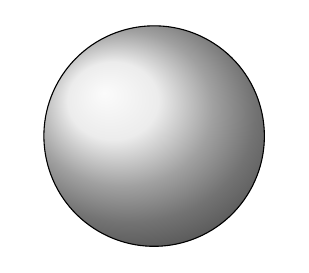
\begin{tikzpicture} % "THE GLOBE" showcase
\begin{scope}[rotate=-30]
\def\R{1.4} % sphere radius
\def\angEl{35} % elevation angle
\filldraw[ball color=gray!20] (0,0) circle (\R);
\foreach \t in {-80,-60,...,80} { \DrawLatitudeCircle[\R]{\t} }
\foreach \t in {-5,-35,...,-175} { \DrawLongitudeCircle[\R]{\t} }
\end{scope}
\end{tikzpicture}
};
\node[](circle3) at ([xshift=5.5em]circle2.east) {
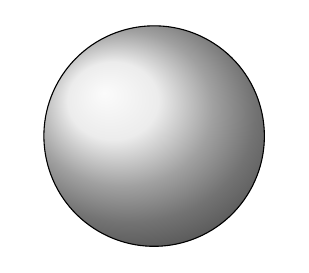
\begin{tikzpicture} % "THE GLOBE" showcase
\begin{scope}[rotate=-30]
\def\R{1.4} % sphere radius
\def\angEl{35} % elevation angle
\filldraw[ball color=gray!20] (0,0) circle (\R);
\foreach \t in {-80,-60,...,80} { \DrawLatitudeCircle[\R]{\t} }
\foreach \t in {-5,-35,...,-175} { \DrawLongitudeCircle[\R]{\t} }
\end{scope}
\end{tikzpicture}
};
\node[](circle4) at ([xshift=5.5em]circle3.east) {
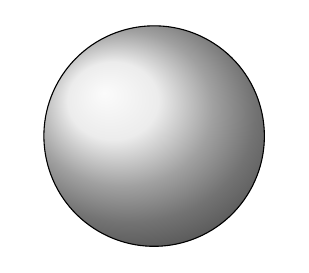
\begin{tikzpicture} % "THE GLOBE" showcase
\begin{scope}[rotate=-30]
\def\R{1.4} % sphere radius
\def\angEl{35} % elevation angle
\filldraw[ball color=gray!20] (0,0) circle (\R);
\foreach \t in {-80,-60,...,80} { \DrawLatitudeCircle[\R]{\t} }
\foreach \t in {-5,-35,...,-175} { \DrawLongitudeCircle[\R]{\t} }
\end{scope}
\end{tikzpicture}
};
\draw[->,very thick] ([xshift=-0.5em]circle2.east)--([xshift=0.5em]circle3.west)node [pos=0.5,above] (pos1) {\scriptsize{$\mathbi{Y}$空间}};
\node [anchor=south](pos1-2) at ([yshift=-0.5em]pos1.north){\scriptsize{\mathbi{X}映射到}};
\draw[->,very thick] ([xshift=-0.5em]circle3.east)--([xshift=0.5em]circle4.west)node [pos=0.5,above] (pos2) {\scriptsize{推断}};
\node [anchor=south](pos2-2) at ([yshift=-0.5em]pos2.north){\scriptsize{词典}};

%circle1
\node[rec,anchor=center,rotate=60,fill=red!20](c1x1) at ([xshift=-7em,yshift=-1.4em]circle1.east){\tiny{1}};
\node[rec,anchor=center,rotate=60,fill=red!20](c1x2) at ([xshift=-4.5em,yshift=1.8em]circle1.east){\tiny{2}};
\node[rec,anchor=center,rotate=60,fill=red!20](c1x3) at ([xshift=-4em,yshift=-0.5em]circle1.east){\tiny{3}};
\node[rec,anchor=center,rotate=60,fill=red!20](c1x4) at ([xshift=-3.5em,yshift=-2.5em]circle1.east){\tiny{4}};
\node[rec,anchor=center,rotate=60,fill=red!20](c1x5) at ([xshift=-2em,yshift=1.0em]circle1.east){\tiny{5}};

%circle2
\node[cir,anchor=center,rotate=-30,fill=blue!20] (c2a) at ([xshift=-5.3em,yshift=2.15em]circle2.east){\tiny{$a$}};
\node[cir,anchor=east,rotate=-30,fill=blue!20] (c2b) at ([xshift=2.0em,yshift=-1.25em]c2a.east){\tiny{$b$}};
\node[cir,anchor=east,rotate=-30,fill=blue!20] (c2c) at ([xshift=0.8em,yshift=-3.9em]c2a.south){\tiny{$c$}};
\node[cir,anchor=east,rotate=-30,fill=blue!20] (c2x) at ([xshift=-0.3em,yshift=-1.9em]c2a.south){\tiny{$x$}};
\node[cir,anchor=west,rotate=-30,fill=blue!20] (c2y) at ([xshift=1.15em,yshift=-2.85em]c2a.east){\tiny{$y$}};

%circle3
\node[rec,anchor=center,rotate=-30,fill=red!20] (c3x1) at ([xshift=-6.7em,yshift=1.75em]circle3.east){\tiny{1}};
\node[rec,anchor=east,rotate=-30,fill=red!20] (c3x2) at ([xshift=4.7em,yshift=-0.95em]c3x1.east){\tiny{2}};
\node[rec,anchor=east,rotate=-30,fill=red!20] (c3x3) at ([xshift=2.6em,yshift=-2.4em]c3x1.south){\tiny{3}};
\node[rec,anchor=east,rotate=-30,fill=red!20] (c3x4) at ([xshift=0.35em,yshift=-2.7em]c3x1.south){\tiny{4}};
\node[rec,anchor=west,rotate=-30,fill=red!20] (c3x5) at ([xshift=2.35em,yshift=-3.85em]c3x1.east){\tiny{5}};

%circle4
\node[rec,anchor=center,rotate=-30,fill=red!20] (c4x1) at ([xshift=-6.7em,yshift=1.75em]circle4.east){\tiny{1}};
\node[rec,anchor=east,rotate=-30,fill=red!20] (c4x2) at ([xshift=4.7em,yshift=-0.95em]c4x1.east){\tiny{2}};
\node[rec,anchor=east,rotate=-30,fill=red!20] (c4x3) at ([xshift=2.6em,yshift=-2.4em]c4x1.south){\tiny{3}};
\node[rec,anchor=east,rotate=-30,fill=red!20] (c4x4) at ([xshift=0.35em,yshift=-2.7em]c4x1.south){\tiny{4}};
\node[rec,anchor=west,rotate=-30,fill=red!20] (c4x5) at ([xshift=2.35em,yshift=-3.85em]c4x1.east){\tiny{5}};

\node[cir,anchor=center,rotate=-30,fill=blue!20] (c4a) at ([xshift=-5.3em,yshift=2.15em]circle4.east){\tiny{$a$}};
\node[cir,anchor=east,rotate=-30,fill=blue!20] (c4b) at ([xshift=2.0em,yshift=-1.25em]c4a.east){\tiny{$b$}};
\node[cir,anchor=east,rotate=-30,fill=blue!20] (c4c) at ([xshift=0.8em,yshift=-3.9em]c4a.south){\tiny{$c$}};
\node[cir,anchor=east,rotate=-30,fill=blue!20] (c4x) at ([xshift=-0.3em,yshift=-1.9em]c4a.south){\tiny{$x$}};
\node[cir,anchor=west,rotate=-30,fill=blue!20] (c4y) at ([xshift=1.15em,yshift=-2.85em]c4a.east){\tiny{$y$}};

\draw [color=red,line width=0.7pt,rotate=18] ([xshift=-5.1em,yshift=3.7em]circle4.east) ellipse (1.6em and 0.9em); 
\draw [color=red,line width=0.7pt,rotate=-5] ([xshift=-2.8em,yshift=0.6em]circle4.east) ellipse (1.6em and 0.9em);
\draw [color=red,line width=0.7pt,rotate=65] ([xshift=-3.10em,yshift=2.10em]circle4.east) ellipse (1.6em and 0.9em);
\draw [color=red,line width=0.7pt,rotate=60] ([xshift=-3.75em,yshift=3.7em]circle4.east) ellipse (1.5em and 0.9em);
\draw [color=red,line width=0.7pt,rotate=65] ([xshift=-3.4em,yshift=5.9em]circle4.east) ellipse (1.5em and 0.9em);

\node [anchor=north](part1) at ([yshift=0.5em]circle1.south){\small{$\mathbi{X}$}};
\node [anchor=west](part2) at ([xshift=6em]part1.east){\small{$\mathbi{Y}$}};
\node [anchor=west](part3) at ([xshift=8.5em]part2.east){\small{$\mathbi{X} \mathbi{W}$}};
\node [anchor=west](part3) at ([xshift=15.0em]part2.east){\small{$\mathbi{X} \mathbi{W}$和$\mathbi{Y}$在同一空间}};

\node [anchor=center](c1) at (5.4,-1.0){\small{$\mathbi{W}$}};

\draw[->,thick] (5.8,-1.2)..controls (5.5,-1.5) and(5.2,-1.2) ..(5.2,-1.2)..controls (4.9,-0.9) and (5.2,-0.6)..(5.5,-0.6);


\end{tikzpicture}

\caption{词典归纳原理图}
\label{fig:16-16}
\end{figure}
%----------------------------------------------

\parinterval 研究人员也提出了完全无监督的词典归纳方法,这类方法不依赖于任何种子词典即可实现词典归纳,下面进行介绍。

%----------------------------------------------------------------------------------------
%    NEW SUB-SUB-SECTION
%----------------------------------------------------------------------------------------
\subsubsection{1. 基本框架}

\parinterval 无监督词典归纳的核心思想是充分利用词嵌入空间近似同构的假设\upcite{DBLP:conf/emnlp/XuYOW18},基于一些无监督匹配的方法来得到一个初始化的种子词典,之后利用该种子词典作为起始监督信号不断进行微调进一步提高性能。总结起来,无监督词典归纳系统通常包括以下两个阶段:

\begin{itemize}
\vspace{0.5em}
\item {\small\bfnew{基于无监督的分布匹配}}。该阶段利用一些无监督的方法来得到一个包含噪声的初始化词典$D$。
\vspace{0.5em}
\item {\small\bfnew{基于有监督的微调}}。利用两个单语词嵌入和第一阶段中学习到的种子字典执行一些对齐算法来迭代微调,例如,{\small\bfnew{普氏分析}}\index{普氏分析}(Procrustes Analysis\index{Procrustes Analysis})\upcite{1966ASchnemann}。
\vspace{0.5em}
\end{itemize}

\parinterval 其具体流程如图\ref{fig:16-17}所示,主要步骤包括:

\begin{itemize}
\vspace{0.5em}
\item 对于图\ref{fig:16-17}(a)中的分布在不同空间中的两个单语词嵌入$\mathbi{X}$和$\mathbi{Y}$,基于两者近似同构的假设,利用无监督匹配的方法来得到一个粗糙的线性映射$\mathbi{W}$,使得两个空间能大致对齐,结果如图\ref{fig:16-17}(b)所示。
\vspace{0.5em}
\item 在这个共享空间中执行对齐算法从而归纳出一个种子词典,如图\ref{fig:16-17}(c)所示。
\vspace{0.5em}
\item 利用种子词典不断迭代微调进一步提高映射$\mathbi{W}$的性能,最终映射的效果如图\ref{fig:16-17}(d)所示,之后即可从中推断出词典,并作为最后的结果。
\vspace{0.5em}
\end{itemize}
%----------------------------------------------
\begin{figure}[h]
\centering
\begin{tikzpicture}

%%%%%%%%词典推断------------------------------------------------------------
\begin{scope}
\draw [-,ublue,line width=0.5pt] (0,0)..controls (0.3,0.2) and (0.5,0)..(0.7,-0.2)..controls (0.8,-0.3) and (0.9,-0.4)..(1.1,-0.4)..controls (1.3,-0.4) and (1.3,-0.1)..(1.28,0)..controls (1.26,0.1) and (1.25,0.2)..(1.2,0.3)..controls (1.15,0.4)and (1.2,0.5)..(1.6,0.55)..controls (1.7,0.56) and (1.78,0.5)..(1.85,0.35)..controls (2.0,0.0) and (2.05,-0.1)..(2.05,-0.5)..controls (2.04,-1.1) and (1.5,-1.1)..(0.6,-0.78)..controls (0.5,-0.74) and (0.4,-0.7)..(0.2,-0.5)..controls(0.1,-0.4) and (-0.15,-0.1)..(0,0) ;

\draw [-,red!70,line width=0.5pt] (0.04,-0.5) .. controls (0,-0.4) and (0.4,-0.1)..(0.7,-0.3)..controls (0.9,-0.45) and (1.1,-0.4)..(1.2,-0.3)..controls (1.3,-0.2) and (1.2,0.1).. (1.0,0.3)..controls (0.8,0.5) and (1.0,0.6)..(1.2,0.67)..controls (1.5,0.78) and (1.8,0.5)..(1.9,0.2)..controls(2.1,-0.3) and (2,-0.5)..(1.8,-0.75)..controls (1.5,-1.1) and (1.2,-1.0)..(0.4,-0.8)..controls (0.3,-0.77) and (0.14,-0.755)..(0.04,-0.5);

\draw [-,thick] (-0.7,1.0)--(-0.7,-1.0);

\node [anchor=center](c1) at (-0.1,0){\tiny{$\mathbi{Y}$}};
\node [anchor=center](c2) at (-0.3,-0.7){\tiny{$\mathbi{W} \mathbi{X}$}};
\node [anchor=center,red!70](cr1) at (0.65,-0.65){\scriptsize{$\bullet$}}; 
\node [anchor=center,ublue](cb1) at (0.6,-0.5){\scriptsize{$\bullet$}};
\node [anchor=center,red!70](cr2) at (1.65,-0.65){\scriptsize{$\bullet$}}; 
\node [anchor=center,ublue](cb2) at (1.55,-0.8){\scriptsize{$\bullet$}};
\node [anchor=center,red!70](cr3) at (1.5,0.1){\scriptsize{$\bullet$}}; 
\node [anchor=center,ublue](cb3) at (1.6,-0.05){\scriptsize{$\bullet$}}; 
\draw [-,red](0.65,-0.65)--(0.60,-0.62)--(0.66,-0.58)--(0.6,-0.55)--(0.63,-0.52)--(0.6,-0.5);
\draw [-,red](1.65,-0.65)--(1.60,-0.68)--(1.64,-0.72)--(1.56,-0.72)--(1.60,-0.76)--(1.55,-0.8);
\draw [-,red](1.5,0.1)--(1.53,0.08)--(1.49,0.04)--(1.58,0.03)--(1.54,-0.01)--(1.6,-0.05);
\end{scope}

%%%%%%%%X映射到Y空间------------------------------------------------------------
\begin{scope}[xshift=-8.0em]
\draw [-,ublue,line width=0.5pt] (0,0)..controls (0.3,0.2) and (0.5,0)..(0.7,-0.2)..controls (0.8,-0.3) and (0.9,-0.4)..(1.1,-0.4)..controls (1.3,-0.4) and (1.3,-0.1)..(1.28,0)..controls (1.26,0.1) and (1.25,0.2)..(1.2,0.3)..controls (1.15,0.4)and (1.2,0.5)..(1.6,0.55)..controls (1.7,0.56) and (1.78,0.5)..(1.85,0.35)..controls (2.0,0.0) and (2.05,-0.1)..(2.05,-0.5)..controls (2.04,-1.1) and (1.5,-1.1)..(0.6,-0.78)..controls (0.5,-0.74) and (0.4,-0.7)..(0.2,-0.5)..controls(0.1,-0.4) and (-0.15,-0.1)..(0,0) ;

\draw [-,red!70,line width=0.5pt] (0.04,-0.5) .. controls (0,-0.4) and (0.4,-0.1)..(0.7,-0.3)..controls (0.9,-0.45) and (1.1,-0.4)..(1.2,-0.3)..controls (1.3,-0.2) and (1.2,0.1).. (1.0,0.3)..controls (0.8,0.5) and (1.0,0.6)..(1.2,0.67)..controls (1.5,0.78) and (1.8,0.5)..(1.9,0.2)..controls(2.1,-0.3) and (2,-0.5)..(1.8,-0.75)..controls (1.5,-1.1) and (1.2,-1.0)..(0.4,-0.8)..controls (0.3,-0.77) and (0.14,-0.755)..(0.04,-0.5);

\draw [-,thick] (-0.7,1.0)--(-0.7,-1.0);

\node [anchor=center](c1) at (-0.1,0){\tiny{$\mathbi{Y}$}};
\node [anchor=center](c2) at (-0.3,-0.7){\tiny{$\mathbi{W} \mathbi{X}$}};
\node [anchor=center,red!70](cr1) at (0.65,-0.65){\scriptsize{$\bullet$}}; 
\node [anchor=center,ublue](cb1) at (0.6,-0.5){\scriptsize{$\bullet$}};
\node [anchor=center,red!70](cr2) at (1.65,-0.65){\scriptsize{$\bullet$}}; 
\node [anchor=center,ublue](cb2) at (1.55,-0.8){\scriptsize{$\bullet$}};
\node [anchor=center,red!70](cr3) at (1.5,0.1){\scriptsize{$\bullet$}}; 
\node [anchor=center,ublue](cb3) at (1.6,-0.05){\scriptsize{$\bullet$}}; 
%%%%%%一堆红色的球
\node [anchor=center,red!70](cr4) at (0.15,-0.6){\Large{$\cdot$}};
\node [anchor=center,red!70](cr5) at (0.3,-0.6){\Large{$\cdot$}};
\node [anchor=center,red!70](cr6) at (0.5,-0.55){\Large{$\cdot$}};
\node [anchor=center,red!70](cr7) at (0.35,-0.4){\Large{$\cdot$}};
\node [anchor=center,red!70](cr8) at (0.4,-0.7){\Large{$\cdot$}};
\node [anchor=center,red!70](cr8) at (0.55,-0.8){\Large{$\cdot$}};
\node [anchor=center,red!70](cr9) at (0.9,-0.8){\Large{$\cdot$}};
\node [anchor=center,red!70](cr10) at (0.9,-0.5){\Large{$\cdot$}};
\node [anchor=center,red!70](cr11) at (1.4,-0.8){\Large{$\cdot$}};
\node [anchor=center,red!70](cr12) at (1.45,-0.3){\Large{$\cdot$}};
\node [anchor=center,red!70](cr13) at (1.35,0.3){\Large{$\cdot$}};
\node [anchor=center,red!70](cr14) at (1.2,0.4){\Large{$\cdot$}};
\node [anchor=center,red!70](cr15) at (1.6,0.45){\Large{$\cdot$}};
%%%%%%一堆蓝色的球
\node [anchor=center,ublue](cb4) at (0.1,-0.2){\Large{$\cdot$}};
\node [anchor=center,ublue](cb5) at (0.3,-0.2){\Large{$\cdot$}};
\node [anchor=center,ublue](cb6) at (0.5,-0.25){\Large{$\cdot$}};
\node [anchor=center,ublue](cb7) at (0.4,-0.1){\Large{$\cdot$}};
\node [anchor=center,ublue](cb8) at (0.35,-0.45){\Large{$\cdot$}};
\node [anchor=center,ublue](cb9) at (0.45,-0.6){\Large{$\cdot$}};
\node [anchor=center,ublue](cb10) at (0.85,-0.45){\Large{$\cdot$}};
\node [anchor=center,ublue](cb11) at (1.45,-0.45){\Large{$\cdot$}};
\node [anchor=center,ublue](cb12) at (1.3,-0.85){\Large{$\cdot$}};
\node [anchor=center,ublue](cb13) at (1.8,-0.5){\Large{$\cdot$}};
\node [anchor=center,ublue](cb14) at (1.75,0.2){\Large{$\cdot$}};
\node [anchor=center,ublue](cb15) at (1.6,0.2){\Large{$\cdot$}};
\end{scope}

%%%%%%%%X、Y词嵌入空间------------------------------------------------------------
\begin{scope}[xshift=-16em]
\draw [-,ublue,line width=0.5pt] (0,0)..controls (0.3,0.2) and (0.5,0)..(0.7,-0.2)..controls (0.8,-0.3) and (0.9,-0.4)..(1.1,-0.4)..controls (1.3,-0.4) and (1.3,-0.1)..(1.28,0)..controls (1.26,0.1) and (1.25,0.2)..(1.2,0.3)..controls (1.15,0.4)and (1.2,0.5)..(1.6,0.55)..controls (1.7,0.56) and (1.78,0.5)..(1.85,0.35)..controls (2.0,0.0) and (2.05,-0.1)..(2.05,-0.5)..controls (2.04,-1.1) and (1.5,-1.1)..(0.6,-0.78)..controls (0.5,-0.74) and (0.4,-0.7)..(0.2,-0.5)..controls(0.1,-0.4) and (-0.15,-0.1)..(0,0) ;

\node [anchor=center](x1) at (-1.45,0.2){\tiny{$\mathbi{X}$}};
\node [anchor=center](y1) at (1.1,0.1){\tiny{$\mathbi{Y}$}};

\node [anchor=center,ublue](cb1) at (0.6,-0.5){\scriptsize{$\bullet$}};
\node [anchor=center,ublue](cb2) at (1.55,-0.8){\scriptsize{$\bullet$}};
\node [anchor=center,ublue](cb3) at (1.6,-0.05){\scriptsize{$\bullet$}}; 
%%%%%%一堆蓝色的球
\node [anchor=center,ublue](cb4) at (0.1,-0.2){\Large{$\cdot$}};
\node [anchor=center,ublue](cb5) at (0.3,-0.2){\Large{$\cdot$}};
\node [anchor=center,ublue](cb6) at (0.5,-0.25){\Large{$\cdot$}};
\node [anchor=center,ublue](cb7) at (0.4,-0.1){\Large{$\cdot$}};
\node [anchor=center,ublue](cb8) at (0.35,-0.45){\Large{$\cdot$}};
\node [anchor=center,ublue](cb9) at (0.45,-0.6){\Large{$\cdot$}};
\node [anchor=center,ublue](cb10) at (0.85,-0.45){\Large{$\cdot$}};
\node [anchor=center,ublue](cb11) at (1.45,-0.45){\Large{$\cdot$}};
\node [anchor=center,ublue](cb12) at (1.3,-0.85){\Large{$\cdot$}};
\node [anchor=center,ublue](cb13) at (1.8,-0.5){\Large{$\cdot$}};
\node [anchor=center,ublue](cb14) at (1.75,0.2){\Large{$\cdot$}};
\node [anchor=center,ublue](cb15) at (1.6,0.2){\Large{$\cdot$}};

\node [anchor=center](rw1) at (-0.5,0.45){\tiny{cat}}; 
\node [anchor=center](rw2) at (0.05,0.4){\tiny{feline}}; 
\node [anchor=center](rw3) at (-1.17,-0.07){\tiny{car}}; 
\node [anchor=center](rw4) at (-0.7,-0.65){\tiny{deep}};
\node [anchor=center](bw1) at (0.2,-0.1){\tiny{felin}};
\node [anchor=center](bw2) at (0.75,-0.65){\tiny{katze}};
\node [anchor=center](bw3) at (1.55,-0.65){\tiny{auto}};
\node [anchor=center](bw4) at (1.6,-0.2){\tiny{tief}};
\node [anchor=center](de1) at (0.3,-1.5) {\small{(a) $\mathbi{X}$、$\mathbi{Y}$词嵌入空间}};
\node [anchor=center](de2) at (3.9,-1.5) {\small{(b) $\mathbi{X}$映射到$\mathbi{Y}$空间}};
\node [anchor=center](de3) at (7,-1.5) {\small{(c) 词典推断}};
\node [anchor=center](de4) at (10.1,-1.5) {\small{(d) 微调结果}};

\end{scope}

\begin{scope}[xshift=-14.5em,yshift=0.8em,rotate=-150]
\draw [-,red!70,line width=0.5pt] (0.04,-0.5) .. controls (0,-0.4) and (0.4,-0.1)..(0.7,-0.3)..controls (0.9,-0.45) and (1.1,-0.4)..(1.2,-0.3)..controls (1.3,-0.2) and (1.2,0.1).. (1.0,0.3)..controls (0.8,0.5) and (1.0,0.6)..(1.2,0.67)..controls (1.5,0.78) and (1.8,0.5)..(1.9,0.2)..controls(2.1,-0.3) and (2,-0.5)..(1.8,-0.75)..controls (1.5,-1.1) and (1.2,-1.0)..(0.4,-0.8)..controls (0.3,-0.77) and (0.14,-0.755)..(0.04,-0.5);

\node [anchor=center,red!70](cr1) at (0.65,-0.65){\scriptsize{$\bullet$}}; 
\node [anchor=center,red!70](cr2) at (1.65,-0.65){\scriptsize{$\bullet$}}; 
\node [anchor=center,red!70](cr3) at (1.5,0.1){\scriptsize{$\bullet$}}; 
%%%%%%一堆红色的球
\node [anchor=center,red!70](cr4) at (0.15,-0.6){\Large{$\cdot$}};
\node [anchor=center,red!70](cr5) at (0.3,-0.6){\Large{$\cdot$}};
\node [anchor=center,red!70](cr6) at (0.5,-0.55){\Large{$\cdot$}};
\node [anchor=center,red!70](cr7) at (0.35,-0.4){\Large{$\cdot$}};
\node [anchor=center,red!70](cr8) at (0.4,-0.7){\Large{$\cdot$}};
\node [anchor=center,red!70](cr8) at (0.55,-0.8){\Large{$\cdot$}};
\node [anchor=center,red!70](cr9) at (0.9,-0.8){\Large{$\cdot$}};
\node [anchor=center,red!70](cr10) at (0.9,-0.5){\Large{$\cdot$}};
\node [anchor=center,red!70](cr11) at (1.4,-0.8){\Large{$\cdot$}};
\node [anchor=center,red!70](cr12) at (1.45,-0.3){\Large{$\cdot$}};
\node [anchor=center,red!70](cr13) at (1.35,0.3){\Large{$\cdot$}};
\node [anchor=center,red!70](cr14) at (1.2,0.4){\Large{$\cdot$}};
\node [anchor=center,red!70](cr15) at (1.6,0.45){\Large{$\cdot$}};
\end{scope}

%%%%%%%%%%%微调结果------------------------------------------------------------
\begin{scope}[xshift=8.2em]
\draw [-,red!70,line width=0.5pt] (0,0.4688)..controls (0.3,0.45) and (0.5,0.2)..(0.7,-0.25)..controls (0.8,-0.45) and (0.9,-0.4)..(1.1,-0.4)..controls (1.3,-0.42) and (1.3,-0.12)..(1.28,0)..controls (1.26,0.1) and (1.25,0.2)..(1.2,0.3)..controls (1.13,0.4) and (1.18,0.5)..(1.6,0.55)..controls (1.7,0.56) and (1.78,0.5)..(1.85,0.35)..controls (2.03,0.0) and (2.08,-0.1)..(2.07,-0.5)..controls (2.04,-1.1) and (1.5,-1.16)..(0.6,-0.91)..controls (0.05,-0.71) and (-0.2,-0.53)..(-0.25,-0.45)..controls (-0.55,0.0) and (-0.5,0.501)..(0,0.4688);

\draw [-,ublue,line width=0.5pt] (0,0.5)..controls (0.3,0.5) and (0.5,0.2)..(0.7,-0.25)..controls (0.8,-0.45) and (0.9,-0.4)..(1.1,-0.4)..controls (1.3,-0.40) and (1.3,-0.1)..(1.28,0)..controls (1.26,0.1) and (1.25,0.2)..(1.2,0.3)..controls (1.15,0.4)and (1.2,0.5)..(1.6,0.55)..controls (1.7,0.56) and (1.78,0.5)..(1.85,0.35)..controls (2.0,0.0) and (2.05,-0.1)..(2.05,-0.5)..controls (2.04,-1.1) and (1.5,-1.1)..(0.6,-0.91)..controls (0.0,-0.75) and (-0.2,-0.53)..(-0.25,-0.45)..controls (-0.5,0.0) and (-0.5,0.501)..(0,0.5);

\draw [-,thick] (-0.8,1.0)--(-0.8,-1.0);

\node [anchor=center](c1) at (0.1,0.6){\tiny{$\mathbi{Y}$}};
\node [anchor=center](c2) at (-0.45,-0.7){\tiny{$\mathbi{W} \mathbi{X}$}};

\node [anchor=center,red!70](cr1) at (0.2,-0.35){\scriptsize{$\bullet$}};
\node [anchor=center,red!70](cr2) at (1.58,-0.78){\scriptsize{$\bullet$}};
\node [anchor=center,red!70](cr3) at (1.6,0){\scriptsize{$\bullet$}}; 

\node [anchor=center,ublue](cb1) at (0.2,-0.3){\scriptsize{$\bullet$}};
\node [anchor=center,ublue](cb2) at (1.55,-0.8){\scriptsize{$\bullet$}};
\node [anchor=center,ublue](cb3) at (1.6,-0.05){\scriptsize{$\bullet$}}; 
%%%%%%一堆红色的球
\node [anchor=center,red!70](cb4) at (-0.35,0.16){\Large{$\cdot$}};
\node [anchor=center,red!70](cb5) at (-0.03,0.37){\Large{$\cdot$}};
\node [anchor=center,red!70](cb6) at (-0.03,0.12){\Large{$\cdot$}};
\node [anchor=center,red!70](cb7) at (0.37,0.02){\Large{$\cdot$}};
\node [anchor=center,red!70](cb8) at (-0.18,-0.18){\Large{$\cdot$}};
\node [anchor=center,red!70](cb9) at (0.65,-0.43){\Large{$\cdot$}};
\node [anchor=center,red!70](cb10) at (0.32,-0.68){\Large{$\cdot$}};
\node [anchor=center,red!70](cb11) at (0.82,-0.73){\Large{$\cdot$}};
\node [anchor=center,red!70](cb12) at (1.23,-0.85){\Large{$\cdot$}};
\node [anchor=center,red!70](cb13) at (1.8,-0.47){\Large{$\cdot$}};
\node [anchor=center,red!70](cb14) at (1.75,0.23){\Large{$\cdot$}};
\node [anchor=center,red!70](cb15) at (1.38,-0.44){\Large{$\cdot$}};
\node [anchor=center,red!70](cb16) at (1.42,0.26){\Large{$\cdot$}};
%%%%%%一堆蓝色的球
\node [anchor=center,ublue](cb4) at (-0.35,0.2){\Large{$\cdot$}};
\node [anchor=center,ublue](cb5) at (0,0.4){\Large{$\cdot$}};
\node [anchor=center,ublue](cb6) at (0,0.15){\Large{$\cdot$}};
\node [anchor=center,ublue](cb7) at (0.4,0.05){\Large{$\cdot$}};
\node [anchor=center,ublue](cb8) at (-0.15,-0.15){\Large{$\cdot$}};
\node [anchor=center,ublue](cb9) at (0.65,-0.4){\Large{$\cdot$}};
\node [anchor=center,ublue](cb10) at (0.3,-0.65){\Large{$\cdot$}};
\node [anchor=center,ublue](cb11) at (0.8,-0.7){\Large{$\cdot$}};
\node [anchor=center,ublue](cb12) at (1.2,-0.85){\Large{$\cdot$}};
\node [anchor=center,ublue](cb13) at (1.8,-0.5){\Large{$\cdot$}};
\node [anchor=center,ublue](cb14) at (1.75,0.2){\Large{$\cdot$}};
\node [anchor=center,ublue](cb15) at (1.4,-0.45){\Large{$\cdot$}};
\node [anchor=center,ublue](cb16) at (1.45,0.3){\Large{$\cdot$}};
\node [anchor=center](rw1) at (0.22,-0.45){\tiny{cat}};
\node [anchor=center](rw2) at (0.20,-0.15){\tiny{katze}};
\end{scope}

\end{tikzpicture}
\caption{无监督词典归纳流程图\upcite{DBLP:conf/iclr/LampleCRDJ18}}
\label{fig:16-17}
\end{figure}
%----------------------------------------------

\parinterval 不同的无监督方法最大的区别主要在于第一阶段,获得初始种子词典的手段,而第二阶段微调的原理都大同小异。第一阶段的主流方法主要有两大类:

\begin{itemize}
\vspace{0.5em}
\item {\small\bfnew{基于生成对抗网络的方法}}\upcite{DBLP:conf/iclr/LampleCRDJ18,DBLP:conf/acl/ZhangLLS17,DBLP:conf/emnlp/XuYOW18,DBLP:conf/naacl/MohiuddinJ19}。在这个方法中,通过生成器来产生映射$\mathbi{W}$,鉴别器负责区分随机抽样的元素$\mathbi{W} \mathbi{X}$ 和$\mathbi{Y}$,两者共同优化收敛后即可得到映射$\mathbi{W}$。
\vspace{0.5em}
\item {\small\bfnew{基于Gromov-wasserstein 的方法}}\upcite{DBLP:conf/emnlp/Alvarez-MelisJ18,DBLP:conf/lrec/GarneauGBDL20,DBLP:journals/corr/abs-1811-01124,DBLP:conf/emnlp/XuYOW18}。Wasserstein距离是度量空间中定义两个概率分布之间距离的函数。在这个任务中,它用来衡量不同语言中单词对之间的相似性,利用空间近似同构的信息可以定义出一些目标函数,之后通过优化该目标函数也可以得到映射$\mathbi{W}$。
\vspace{0.5em}
\end{itemize}

\parinterval 在得到映射$\mathbi{W}$之后,对于$\mathbi{X}$中的任意一个单词$x_{i}$,通过$\mathbi{W} \mathbi{E}({x}_{i})$将其映射到空间$\mathbi{Y}$中($\mathbi{E}({x}_{i})$表示的是单词$x_{i}$的词嵌入向量),然后在$\mathbi{Y}$中找到该点的最近邻点$y_{j}$,于是$y_{j}$就是$x_{i}$的翻译词,重复该过程即可归纳出种子词典$D$,第一阶段结束。事实上,由于第一阶段缺乏监督信号,得到的种子词典$D$会包含大量的噪音,因此需要进行进一步的微调。

\parinterval 微调的原理普遍基于普氏分析\upcite{DBLP:journals/corr/MikolovLS13}。假设现在有一个种子词典$D=\left\{x_{i}, y_{i}\right\}$其中${i \in\{1, n\}}$,和两个单语词嵌入$\mathbi{X}$和$\mathbi{Y}$,那么就可以将$D$作为{\small\bfnew{映射锚点}}\index{映射锚点}(Anchor\index{Anchor})学习一个转移矩阵$\mathbi{W}$,使得$\mathbi{W} \mathbi{X}$与$\mathbi{Y}$这两个空间尽可能相近,此外通过对$\mathbi{W}$施加正交约束可以显著提高性能\upcite{DBLP:conf/naacl/XingWLL15},于是这个优化问题就转变成了{\small\bfnew{普鲁克问题}}\index{普鲁克问题}(Procrustes Problem\index{Procrustes Problem})\upcite{DBLP:conf/iclr/SmithTHH17},可以通过{\small\bfnew{奇异值分解}}\index{奇异值分解}(Singular Value Decomposition,SVD\index{Singular Value Decomposition})来获得近似解。这里用$\mathbi{X}'$和$\mathbi{Y}'$表示$D$中源语言单词和目标语言单词的词嵌入矩阵,优化$\mathbi{W}$的过程可以被描述为:

\begin{eqnarray}
\widehat{\mathbi{W}} & = & \argmin_{\mathbi{W} \in O_{d}(\mathbb{R})}{\|\mathbi{W} \mathbi{X}'- \mathbi{Y}' \|_{\mathrm{F}}} \nonumber \\
                              & = & \mathbi{U} \mathbi{V}^{\rm{T}} \\ \label{eq:16-8}
\textrm{s.t.\ \ \ \ } \mathbi{U} \Sigma \mathbi{V}^{\rm{T}} &= &\operatorname{SVD}\left(\mathbi{Y}' \mathbi{X}'^{\rm{T}}\right)
\label{eq:16-9}
\end{eqnarray}

\noindent 其中, $\|\cdot\|_{\mathrm{F}}$表示矩阵的Frobenius范数,即矩阵元素绝对值的平方和再开方,$d$是词嵌入的维度,$O_d(\mathbb{R})$表示$d\times d$的实数空间,$\operatorname{SVD}(\cdot)$表示奇异值分解。利用上式可以获得新的$\mathbi{W}$,通过$\mathbi{W}$可以归纳出新的$D$,如此迭代进行微调最后即可以得到收敛的$D$。

\parinterval 较早的无监督方法是基于生成对抗网络的方法\upcite{DBLP:conf/acl/ZhangLLS17,DBLP:conf/emnlp/ZhangLLS17,DBLP:conf/iclr/LampleCRDJ18},这是一个很自然的想法,利用生成器产生单词间的映射,然后用判别器来区别两个空间。然而研究表明生成对抗网络缺乏稳定性,容易在低资源语言对上失败\upcite{hartmann2018empirical},因此有不少改进的工作,比如:利用{\small\bfnew{变分自编码器}}\index{变分自编码器}(Variational Autoencoders,VAEs)\index{Variational Autoencoders}来捕获更深层次的语义信息并结合对抗训练的方法\upcite{DBLP:conf/emnlp/DouZH18,DBLP:conf/naacl/MohiuddinJ19};通过改进最近邻点的度量函数来提升性能的方法\upcite{DBLP:conf/acl/HuangQC19,DBLP:conf/emnlp/JoulinBMJG18};利用多语言信号来提升性能的方法\upcite{DBLP:conf/emnlp/ChenC18,DBLP:conf/emnlp/TaitelbaumCG19,DBLP:journals/corr/abs-1811-01124,DBLP:conf/naacl/HeymanVVM19};也有一些工作舍弃生成对抗网络,通过直接优化空间距离来进行单词的匹配\upcite{DBLP:conf/emnlp/HoshenW18,DBLP:conf/emnlp/XuYOW18,DBLP:conf/emnlp/Alvarez-MelisJ18,DBLP:conf/emnlp/MukherjeeYH18}。

%----------------------------------------------------------------------------------------
%    NEW SUB-SUB-SECTION
%----------------------------------------------------------------------------------------
\subsubsection{2. 健壮性问题}

\parinterval 目前很多无监督词典归纳方法在相似语言对比如英-法、英-德上已经取得不错的结果,然而在远距离语言对比如英-中,英-日上的性能仍然很差\upcite{DBLP:conf/emnlp/VulicGRK19,A2020Li}。研发健壮的无监督词典归纳方法仍然存在挑战。因此研发健壮的无监督词典归纳方法仍然面临许多挑战:

\begin{itemize}
\vspace{0.5em}
\item 词典归纳依赖于基于大规模单语数据训练出来的词嵌入,而词嵌入会受到单语数据的来源、数量、词向量训练算法、超参数配置等多方面因素的影响,这很容易导致不同情况下词嵌入结果的差异很大。
\vspace{0.5em}

\item 词典归纳强烈依赖于词嵌入空间近似同构的假设,然而许多语言之间天然的差异导致该假设并不成立。因为无监督系统通常是基于两阶段的方法,起始阶段由于缺乏监督信号很难得到质量较高的种子词典,进而导致后续阶段无法完成准确的词典归纳\upcite{DBLP:conf/acl/SogaardVR18,A2020Li}。
\vspace{0.5em}

\item 由于词嵌入这种表示方式的局限性,模型无法实现单词多对多的对齐,而且对于一些相似的词或者实体,模型也很难实现对齐。
\vspace{0.5em}
\end{itemize}

\parinterval 无监督方法的健壮性是一个很难解决的问题。对于词典推断这个任务来说,是否有必要进行完全无监督的学习仍然值得商榷。因为其作为一个底层任务,不仅可以利用词嵌入,还可以利用单语、甚至是双语信息。此外,基于弱监督的方法代价也不是很大,只需要数千个词对即可。有了监督信号的引导,健壮性问题就能得到一定的缓解。

%----------------------------------------------------------------------------------------
%    NEW SUB-SECTION 16.4.2
%----------------------------------------------------------------------------------------

\subsection{无监督统计机器翻译}

\parinterval 在无监督词典归纳的基础上,可以进一步得到句子间的翻译,实现无监督机器翻译\upcite{DBLP:journals/talip/MarieF20}。统计机器翻译作为机器翻译的主流方法,对其进行无监督学习可以帮助构建初始的无监督机器翻译系统,从而进一步帮助训练更为先进的无监督神经机器翻译系统。以基于短语的统计机器翻译为例,系统主要包含短语表、语言模型、调序模型以及权重调优等模块(见{\chapterseven})。其中短语表和模型调优需要双语数据,而语言模型和(基于距离的)调序模型只依赖于单语数据。因此,如果可以通过无监督的方法完成短语表和权重调优,那么就得到了无监督统计机器翻译系统\upcite{DBLP:conf/emnlp/ArtetxeLA18}。

%----------------------------------------------------------------------------------------
%    NEW SUB-SUB-SECTION
%----------------------------------------------------------------------------------------
\subsubsection{1. 无监督短语归纳}

\parinterval 回顾统计机器翻译中的短语表,它类似于一个词典,对一个源语言短语给出相应的译文\upcite{DBLP:conf/ki/ZensON02}。只不过词典的基本单元是词,而短语表的基本单元是短语(或$n$-gram)。此外短语表还提供短语翻译的得分。既然短语表跟词典如此相似,那么很容易就可以把无监督词典归纳的方法移植到短语上,也就是把里面的词替换成短语,就可以无监督地得到短语表。

\parinterval 如\ref{unsupervised-dictionary-induction}节所述,无监督词典归纳的方法依赖于词的分布式表示,也就是词嵌入。因此当把无监督词典归纳拓展到短语上时,首先需要获得短语的分布式表示。比较简单的方法是把词换成短语,然后借助与无监督词典归纳相同的算法得到短语的分布式表示。最后直接应用无监督词典归纳方法,得到源语言短语与目标语言短语之间的对应。

\parinterval 在得到了短语翻译的基础上,需要确定短语翻译的得分。在无监督词典归纳中,在推断词典的时候会为一对源语言单词和目标语言单词打分(词嵌入之间的相似度),再根据打分来决定哪一个目标语言单词更有可能是当前源语言单词的翻译。在无监督短语归纳中,这样一个打分已经提供了对短语对质量的度量,因此经过适当的归一化处理后就可以得到短语翻译的得分。

%----------------------------------------------------------------------------------------
%    NEW SUB-SUB-SECTION
%----------------------------------------------------------------------------------------
\subsubsection{2. 无监督权重调优}

\parinterval 有了短语表之后,剩下的问题是如何在没有双语数据的情况下进行模型调优,从而把短语表、语言模型、调序模型等模块融合起来\upcite{DBLP:conf/acl/Och03}。在统计机器翻译系统中,短语表可以提供短语的翻译,而语言模型可以保证从短语表中翻译拼装得到的句子的流畅度,因此统计机器翻译模型即使在没有权重调优的基础上也已经具备了一定的翻译能力。所以一个简单而有效的无监督方法就是使用未经过模型调优的统计机器翻译模型进行回译,也就是将目标语言句子翻译成源语言句子后,再将翻译得到的源语句言子当成输入而目标语言句子当成标准答案,完成权重调优。

\parinterval 经过上述的无监督模型调优后,就获得了一个效果更好的翻译模型。这时候,可以使用这个翻译模型去产生质量更高的数据,再用这些数据来继续对翻译模型进行调优,如此反复迭代一定次数后停止。这个方法也被称为{\small\bfnew{迭代优化}}\index{迭代优化}(Iterative Refinement\index{Iterative Refinement})\upcite{DBLP:conf/emnlp/ArtetxeLA18}。

\parinterval 迭代优化也会带来另外一个问题:在每一次迭代中都会产生新的模型,应该什么时候停止生成新模型,挑选哪一个模型呢?因为在无监督的场景当中,没有任何真实的双语数据可以使用,所以无法使用监督学习里的校验集来对每个模型进行检验并筛选。另外,即使有很少量的双语数据(比如数百条双语句对),直接在上面挑选模型和调整超参数会导致过拟合问题,使得最后结果越来越差。一个经验上非常高效的模型选择方法是:事先从训练集里挑选一部分句子作为校验集不参与训练,再使用当前的模型把这些句子翻译过去之后再翻译回来(源语言$\to $目标语言$\to$源语言,或者目标语言$\to$源语言$\to$目标语言),得到的结果跟原始的结果计算BLEU的值,得分越高则效果越好。这种方法已被证明跟使用大规模双语校验集的结果是高度相关的\upcite{DBLP:conf/emnlp/LampleOCDR18}。

%----------------------------------------------------------------------------------------
%    NEW SUB-SECTION
%----------------------------------------------------------------------------------------

\subsection{无监督神经机器翻译}\label{unsupervised-NMT}

\parinterval 既然神经机器翻译已经在很多任务上优于统计机器翻译,为什么不直接做无监督神经机器翻译呢?实际上,由于神经网络的黑盒特性使其无法像统计机器翻译那样进行拆解,并定位问题。因此需要借用其它无监督翻译系统来训练神经机器翻译模型。

%----------------------------------------------------------------------------------------
%    NEW SUB-SUB-SECTION
%----------------------------------------------------------------------------------------
\subsubsection{1. 基于无监督统计机器翻译的方法}

\parinterval 一个简单的方法是,借助已经成功的无监督方法来为神经机器翻译模型提供少量双语监督信号。初始的监督信号可能很少或者包含大量噪声,因此需要逐步优化数据来重新训练出更好的模型。这也是目前绝大多数无监督神经机器翻译方法的核心思路。这个方案最简单的实现就是借助已经构建的无监督统计机器翻译模型,用它产生伪双语数据来训练神经机器翻译模型 ,然后进行迭代回译来进行数据优化\upcite{DBLP:conf/acl/ArtetxeLA19}。这个方法的优点是直观,并且性能稳定,容易调试(所有模块都互相独立)。缺点是复杂繁琐,涉及许多超参数调整工作,而且训练代价较大。

%----------------------------------------------------------------------------------------
%    NEW SUB-SUB-SECTION
%----------------------------------------------------------------------------------------
\subsubsection{2. 基于无监督词典归纳的方法}

\parinterval 另一个思路是直接从无监督词典归纳中得到神经机器翻译模型,从而避免繁琐的无监督统计机器翻译模型的训练,同时也避免神经机器翻译模型继承统计机器翻译模型的错误。这种方法的核心就是把翻译看成一个两阶段的过程:

\begin{itemize}
\vspace{0.5em}
\item 首先,无监督词典归纳通过双语词典把一个源语言句子转换成一个不通顺但是意思完整的目标语言句子。
\vspace{0.5em}
\item 然后,把这样一个不通顺的句子改写成一个流畅的句子,同时保留原来的含义,最后达到翻译的目的。
\vspace{0.5em}
\end{itemize}

\parinterval 而第二阶段的改写任务其实也是一个特殊的翻译任务,只不过现在的源语言和目标语言是使用不同的方式表达的同一种语言的句子。因此可以使用神经机器翻译模型来完成这个任务,而且由于这里不涉及双语数据而只需要单语数据,模型的训练也将是无监督的。这样的方法不再需要无监督统计机器翻译,并且适应能力很强。对于新语种,不需要重新训练神经机器翻译模型,只需要训练无监督词典归纳进行词的翻译,再使用相同的模型进行改写。

\parinterval 但是,目前训练数据需要使用其他语种的双语数据来进行构造(把源语言句子里每个词使用双语词典进行翻译作为输入,输出的目标语言句子不变)。虽然可以通过把单语句子根据规则或者随机进行打乱来生成训练数据,但是这些句子与真实的句子差异较大,导致训练-测试不一致的问题。而且这样一个两阶段的过程会产生错误传播的问题,比如无监督词典归纳对一些词进行了错误的翻译,那么这些错误的翻译会被送下一阶段进行改写,因为翻译模型这时候已经无法看到源语言句子来进行修正,所以最终的结果将继承无监督词典归纳的错误\upcite{DBLP:conf/acl/PourdamghaniAGK19}。

%----------------------------------------------------------------------------------------
%    NEW SUB-SUB-SECTION
%----------------------------------------------------------------------------------------
\subsubsection{3. 更深层的融合}

\parinterval 为了获得更好的神经机器翻译模型,可以对训练流程和模型做更深度的整合。{\chapterten}已经介绍,神经机器翻译模型的训练包含两个阶段:初始化和优化。而无监督神经机器翻译的核心思路也对应这两个阶段,因此可以考虑在模型的初始化阶段使用无监督方法提供初始的监督信号,然后不但优化模型的参数,还优化训练使用的数据,从而避免流水线带来的错误传播。其中初始的监督信号可以通过两种方法提供给模型。一种是直接使用无监督方法提供最初的伪双语数据,然后训练最初的翻译模型。另一种则是借助无监督方法来初始化模型,得到最初的翻译模型后,直接使用初始化好的翻译模型产生伪双语数据,然后训练自己,如图\ref{fig:16-18}所示。图\ref{fig:16-18}(a)的一个简单实现是利用无监督词典归纳得到词典,用这个词典对单语数据进行逐词的翻译,得到最初的伪双语数据,再在这些数据上训练最初的翻译模型,最后不断地交替优化数据和模型,得到更好的翻译模型和质量更好的伪数据\upcite{DBLP:conf/iclr/LampleCDR18}。这样的做法通过不断优化训练用的双语数据,摆脱了无监督词典归纳在最初的伪双语数据中遗留下来的错误,同时也避免了使用无监督统计机器翻译模型的代价。图\ref{fig:16-18}(b)的实现则依赖于具体的翻译模型初始化方法,下一节会讨论翻译模型的不同初始化方法。
%----------------------------------------------
\begin{figure}[h]
\centering
\begin{tabular}{c c}

\begin{tikzpicture}
\begin{scope}
% ,minimum height =1em,minimum width=2em
\tikzstyle{circle} = [draw,black,line width=0.6pt,inner sep=3.5pt,rounded corners=4pt,minimum width=2em]
\tikzstyle{word} = [inner sep=3.5pt]

\node[circle,fill=red!20](data) at (0,0) {\small{数据}};
\node[circle,fill=blue!20](model) at ([xshift=5em]data.east) {\small{模型}};
\node[word] (init) at ([xshift=-5em]data.west){\small{初始化}};

\draw[->,thick] (init.east) -- ([xshift=-0.2em]data.west);
\draw [->,thick] ([yshift=1pt]data.north) .. controls +(90:2em) and +(90:2em) .. ([yshift=1pt]model.north) node[above,midway] {\small{参数优化}};
\draw [->,thick] ([yshift=1pt]model.south) .. controls +(-90:2em) and +(-90:2em) .. ([yshift=1pt]data.south) node[below,midway] {\small{数据优化}};

\node[word] at ([xshift=-0.5em,yshift=-4em]data.south){\small{(a) 基于数据的初始化}};

\end{scope}
\end{tikzpicture}
&
\begin{tikzpicture}
\begin{scope}
% ,minimum height =1em,minimum width=2em
\tikzstyle{circle} = [draw,black,line width=0.6pt,inner sep=3.5pt,rounded corners=4pt,minimum width=2em]
\tikzstyle{word} = [inner sep=3.5pt]

\node[circle,fill=red!20](data) at (0,0) {\small{数据}};
\node[circle,fill=blue!20](model) at ([xshift=5em]data.east) {\small{模型}};
\node[word] (init) at ([xshift=5em]model.east){\small{初始化}};

\draw[->,thick] (init.west) -- ([xshift=0.2em]model.east);
\draw [->,thick] ([yshift=1pt]data.north) .. controls +(90:2em) and +(90:2em) .. ([yshift=1pt]model.north) node[above,midway] {\small{参数优化}};
\draw [->,thick] ([yshift=1pt]model.south) .. controls +(-90:2em) and +(-90:2em) .. ([yshift=1pt]data.south) node[below,midway] {\small{数据优化}};

\node[word] at ([xshift=-0.5em,yshift=-4em]model.south){\small{(b) 基于模型的初始化}};

\end{scope}
\end{tikzpicture}

\end{tabular}
\caption{模型参数初始化策略}
\label{fig:16-18}
\end{figure}
%----------------------------------------------

%----------------------------------------------------------------------------------------
%    NEW SUB-SUB-SECTION
%----------------------------------------------------------------------------------------
\subsubsection{4. 其它问题}

\parinterval 一般可以认为,在生成的伪数据上优化模型会使模型变得更好,这时候对这个更好的模型使用数据增强的手段(如回译等)就可以生成更好的训练数据。这样的一个数据优化过程依赖于一个假设:模型经过优化后会生成比原始数据更好的数据。而在数据优化和参数优化的共同影响下,模型非常容易拟合数据中的简单模式,使得模型倾向产生包含这种简单模式的数据,造成模型对这种类型数据过拟合的现象。一个常见的问题就是模型对任何输入都输出相同的译文,这时候翻译模型无法产生任何有意义的结果,也就是,数据优化产生的数据里无论什么目标语言对应的源语言都是同一个句子。这种情况下翻译模型虽然能降低过拟合现象造成的损失,但是它不能学会任何源语言跟目标语言之间的对应关系,也就无法进行正确翻译。这个现象也反映出无监督机器翻译训练的脆弱性。

\parinterval 比较常见的解决方案是在双语数据对应的目标函数外增加一个语言模型的目标函数。因为,在初始阶段,由于数据中存在大量不通顺的句子,额外的语言模型目标函数能把部分句子纠正过来,使得模型逐渐生成更好的数据\upcite{DBLP:conf/emnlp/LampleOCDR18}。这个方法在实际应用中非常有效,尽管目前还没有太多理论上的支持。

\parinterval 无监督神经机器翻译还有两个关键的技巧:
\begin{itemize}
\item {\small\bfnew{词表共享}}:对于源语言和目标语言里都一样的词使用同一个词嵌入,而不是源语言和目标语言各自对应一个词嵌入,比如,阿拉伯数字或者一些实体名字。这样相当于告诉模型这个词在源语言和目标语言里面表达同一个意思,隐式地引入了单词翻译的监督信号。在无监督神经机器翻译里词表共享搭配子词切分会更加有效,因为子词的覆盖范围广,比如,多个不同的词可以包含同一个子词。

\vspace{0.5em}
\item {\small\bfnew{模型共享}}:与多语言翻译系统类似,使用同一个翻译模型来进行正向翻译(源语言$\to$目标语言)和反向翻译(目标语言$\to$源语言)。这样做降低了模型的参数量。而且,两个翻译方向可以互相为对方起到正则化的作用,减小了过拟合的风险。
\end{itemize}

\parinterval 最后图\ref{fig:16-19}简单总结了无监督神经机器翻译的流程。下面分别讨论:无监督神经机器翻译里面模型的初始化,以及语言模型目标函数的选择。
%----------------------------------------------
\begin{figure}[h]
\centering

\begin{tikzpicture}
\begin{scope}
\tikzstyle{circle} = [draw,black,line width=0.6pt,inner sep=3.5pt,rounded corners=4pt,minimum width=2em,align=center,fill=blue!20]
\tikzstyle{word} = [inner sep=3.5pt]

\node[circle](center) at (0,0) {
\begin{tabular}{c | c}
$x\rightarrow y$ & $y\rightarrow x$ \\
\small{模型} & \small{模型}
\end{tabular}
};
\node[circle,fill=red!20] (left) at ([xshift=-9em]center.west) {$x\rightarrow y$ \\ \small{数据}};
\node[circle,fill=red!20] (right) at ([xshift=9em]center.east) {$y\rightarrow x$ \\ \small{数据}};

\node[word] (init) at ([yshift=6em]center.north){\small{初始化}};

\node[circle,fill=red!20] (down) at ([yshift=-8em]center.south) {$x,y$ \\ \small{数据}};

\draw[->,thick] (init.south) -- ([yshift=0.2em]center.north);
\draw[->,thick] ([yshift=0.2em]down.north) -- ([yshift=-0.2em]center.south) node[pos=0.6,midway,align=left,xshift=-2.5em,yshift=0.5em] {\small{语言模型}\\\small{目标函数}};
\node [anchor=center] at ([yshift=2.0em,xshift=-2.5em]down.north){\small{(模型优化)}};
\draw[->,thick] ([yshift=1pt]left.north) .. controls +(90:2em) and +(90:2em) .. ([yshift=1pt,xshift=-2.2em]center.north) node[above,midway,align=center] {\small{翻译模型目标函数}\\\small{(模型优化)}};
\draw[->,thick] ([yshift=1pt,xshift=-1.8em]center.north) .. controls +(90:2em) and +(90:2em) .. ([yshift=1pt]right.north) node[above,pos=0.6,align=center] {\small{回译}\\\small{(数据优化)}};

\draw [->,thick] ([yshift=1pt]right.south) .. controls +(-90:2em) and +(-90:2em) .. ([yshift=1pt,xshift=2.2em]center.south) node[below,midway,align=center] {\small{翻译模型目标函数}\\\small{(模型优化)}};
\draw [->,thick] ([yshift=1pt,xshift=1.8em]center.south) .. controls +(-90:2em) and +(-90:2em) .. ([yshift=1pt]left.south) node[below,pos=0.6,align=center] {\small{回译}\\\small{(数据优化)}};

\end{scope}
\end{tikzpicture}

\caption{无监督神经机器翻译模型训练流程}
\label{fig:16-19}
\end{figure}
%----------------------------------------------

\noindent{\small\bfnew{1)模型参数初始化}}

\parinterval 无监督神经机器翻译的关键在于如何提供最开始的监督信号,从而启动后续的迭代流程。无监督词典归纳已经可以提供一些可靠的监督信号,那么如何在模型初始化中融入这些信息?既然神经机器翻译模型都使用词嵌入作为输入,而且无监督词典归纳也是基于两种语言共享的词嵌入空间,那么可以使用共享词嵌入空间的词嵌入结果来初始化模型的词嵌入层,然后在这个基础上训练模型。比如,两个语言里意思相近的词对应的词嵌入会比其他词更靠近对方\upcite{DBLP:journals/ipm/FarhanTAJATT20}。 为了防止机器翻译训练过程中模型参数的更新会破坏词嵌入中蕴含的信息,通常初始化后会固定模型的词嵌入层不让其更新\upcite{DBLP:conf/emnlp/ArtetxeLA18}。

\parinterval 进一步,无监督神经机器翻译能在提供更少监督信号的情况下启动,也就是可以去除无监督词典归纳这一步骤\upcite{DBLP:conf/nips/ConneauL19}。这时候模型的初始化直接使用共享词表的预训练模型的参数作为起始点。这个预训练模型直接使用前面提到的预训练方法(如MASS)进行训练,区别在于模型的结构需要严格匹配翻译模型。此外,这个模型不仅仅只在一个语言的单语数据上进行训练,而是同时在两个语言的单语数据上进行训练,并且两个语言的词表进行共享。前面提到,在共享词表特别是共享子词词表的情况下,已经隐式地告诉模型源语言和目标语言里一样的(子)词互为翻译,相当于模型使用了少量的监督信号。在这基础上使用两个语言的单语数据进行预训练,通过模型共享进一步挖掘了语言之间共通的部分。因此,使用预训练模型进行初始化后,无监督神经机器翻译模型已经得到大量的监督信号,从而得以不断通过优化来提升模型性能。

\noindent{\small\bfnew{2)语言模型的使用}}

\parinterval 无监督神经机器翻译的一个重要部分就是来自语言模型的目标函数。因为翻译模型本质上是在完成文本生成任务,所以只有文本生成类型的语言模型建模方法才可以应用到无监督神经机器翻译里。比如,给定前文预测下一词就是一个典型的自回归生成任务(见{\chaptertwo}),因此可以应用到无监督神经机器翻译里。但是,目前在预训练里流行的BERT等模型是掩码语言模型\upcite{devlin2019bert},不能直接在无监督神经机器翻译里使用。

\parinterval 另外一个在无监督神经机器翻译中比较常见的语言模型目标函数则是降噪自编码器。它也是文本生成类型的语言模型建模方法。对于一个句子$\seq{x}$,首先使用一个噪声函数$\seq{x}'=\mathrm{noise}(\seq{x})$ 来对$\seq{x}$注入噪声,产生一个质量较差的句子$\seq{x}'$。然后,让模型学习如何从$\seq{x}'$还原出$\seq{x}$。这样的目标函数比预测下一词更贴近翻译任务,因为它是一个序列到序列的映射,并且输入、输出两个序列在语义上是等价的。这里之所以采用$\seq{x}'$而不是$\seq{x}$自己来预测$\seq{x}$,是因为模型可以通过简单的复制输入作为输出来完成从$\seq{x}$预测$\seq{x}$的任务,很难学到有价值的信息。并且在输入中注入噪声会让模型更加健壮,因此模型可以学会如何利用句子中噪声以外的信息来得到正确的输出。通常来说,噪声函数有三种形式,如表\ref{tab:16-1}所示。
%----------------------------------------------
\begin{table}[h]
\centering
\caption{三种噪声加噪方式示例(原句为``我\ 喜欢\ 吃\ 苹果\ 。'')}
\begin{tabular}{l|l|l}
\multicolumn{1}{c|}{噪声函数} & \multicolumn{1}{c|}{描述} & \multicolumn{1}{c}{例子} \\
\hline
\rule{0pt}{15pt}交换 & 句子中任意两个词进行交换 & ``我\ 喜欢\ \underline{苹果}\ \underline{吃}\ 。'' \\
\rule{0pt}{15pt}删除 & 句子中的词按一定概率被删除 & ``我\ 喜欢\ 吃\ 。'' \\
\rule{0pt}{15pt}空白 & 句子中的词按一定概率被替换成空白符 & ``我\ \underline{\ \ \ \ \ \ \ \ }\ 吃\ 苹果\ 。'' \\
\end{tabular}
\label{tab:16-1}
\end{table}
%----------------------------------------------

\parinterval 实际应用中以上三种形式的噪声函数都会被使用到,其中在交换方法中距离越近的词越容易被交换,并且要保证交换次数有上限,而删除和空白方法里词的删除和替换概率通常都非常低,如$0.1$ 等。

%----------------------------------------------------------------------------------------
%    NEW SECTION 16.5
%----------------------------------------------------------------------------------------
\sectionnewpage
\section{领域适应}

\parinterval 机器翻译常常面临训练时与应用时所处领域不一致的问题,比如,将一个在新闻类数据上训练的翻译系统应用在医学文献翻译任务上。不同领域的句子通常存在着很大的区别,比如,日常用语的结构较为简单,而在化学领域的学术论文中,单词和句子结构较为复杂。此外,不同领域之间存在着较为严重的一词多义问题,即同一个词在不同领域中经常会有不同的含义。实例\ref{eg:16-1}展示了英语单词pitch在不同领域的不同词义。
%----------------------------------------------
\begin{example}
单词pitch在不同领域的不同词义

体育领域:The rugby tour was a disaster both on and off the {\red{pitch}}.

\qquad\qquad \hspace{0.8em} 这次橄榄球巡回赛在{\red{场}}上、{\red{场}}下都彻底失败。

 化学领域:The timbers of similar houses were painted with {\red{pitch}}.

\qquad\qquad \hspace{0.8em} 类似房屋所用的栋木刷了{\red{沥青}}。

 声学领域:A basic sense of rhythm and {\red{pitch}} is essential in a music teacher.

\qquad\qquad \hspace{0.8em} 基本的韵律感和{\red{音高}}感是音乐教师的必备素质。
\label{eg:16-1}
\end{example}
%----------------------------------------------

\parinterval 在机器翻译任务中,新闻等领域的双语数据相对容易获取,所以机器翻译在这些领域上表现较佳。然而,即使在富资源语种上,化学、医学等专业领域的双语数据也十分有限。如果直接使用这些低资源领域的数据来训练机器翻译模型,由于数据稀缺问题,会导致模型的性能较差\upcite{DBLP:conf/iccv/SunSSG17}。如果混合多个领域的数据增大训练数据规模,不同领域数据量之间的不平衡会导致数据较少的领域训练不充分,使得在低资源领域上的翻译结果不尽人意\upcite{DBLP:conf/acl/DuhNST13}。

\parinterval 领域适应方法是利用源领域的知识来改进目标领域模型效果的方法,该方法可以有效地减少模型对目标领域数据的依赖。领域适应主要有两类方法:

\begin{itemize}
\vspace{0.5em}
\item {\small\bfnew{基于数据的方法}}。利用源领域的双语数据或目标领域单语数据进行数据选择或数据增强,来增加模型训练的数据量。
\vspace{0.5em}
\item {\small\bfnew{基于模型的方法}}。针对领域适应开发特定的模型结构、训练策略和推断方法。
\vspace{0.5em}
\end{itemize}

%----------------------------------------------------------------------------------------
%    NEW SUB-SECTION
%----------------------------------------------------------------------------------------
\subsection{基于数据的方法}
\label{sec:domain-adaptatoin-data-based-method}

\parinterval 在统计机器翻译时代,如何有效利用外部数据来改善目标领域的翻译效果已经备受关注
。其中的绝大多数方法与翻译模型无关,因此这些方法也同样适用于神经机器翻译。基于数据的领域适应可以分为基于数据加权的方法、基于数据选择的方法、基于伪数据的方法。图\ref{fig:16-20}展示了这几种方法的示意图。

%----------------------------------------------
\begin{figure}[h]
\centering

\begin{tikzpicture}[scale=0.8]
\begin{scope}
\tikzstyle{data} = [draw,black,very thick,inner sep=2pt,rounded corners=0pt,minimum width=2.5em,minimum height=1.5em,anchor=west]
\tikzstyle{model} = [draw,black,very thick,inner sep=3.5pt,rounded corners=0pt,fill=red!20,minimum width=3em,minimum height=1.5em,font=\footnotesize]
\tikzstyle{word} = [inner sep=3.5pt,align=left,font=\scriptsize]
\tikzstyle{more} = [inner sep=2pt,rounded corners=0pt,minimum width=2.5em,minimum height=1.5em,anchor=west]

\node[data,fill=blue!20] (one) at (0,0) {};
\node[data,fill=green!20] (two) at ([xshift=-0.2em]one.east) {};
\node[data,fill=yellow!20] (three) at ([xshift=-0.2em]two.east) {};

\node[data,fill=blue!20,minimum width=1em] (one_) at ([yshift=-6em]one.south west) {};
\node[data,fill=green!20,minimum width=4.5em] (two_) at ([xshift=-0.2em]one_.east) {};
\node[data,fill=yellow!20,minimum width=2em] (three_) at ([xshift=-0.2em]two_.east) {};

\node[model] (mo) at ([xshift=0.5em,yshift=-5em]two_.south){模型};

\node[word] at ([xshift=-1.5em]one.west) {原始 \\ 数据};
\node[word] at ([xshift=-1.5em]one_.west) {加权};

\node[word,font=\tiny] at ([yshift=1em]one.north) {$(x_1,y_1)$};
\node[word,font=\tiny] at ([yshift=1em]two.north) {$(x_2,y_2)$};
\node[word,font=\tiny] at ([yshift=1em]three.north) {$(x_3,y_3)$};

\node[word,font=\tiny] at ([yshift=1em]one_.north) {$(x_1,y_1)$};
\node[word,font=\tiny] at ([yshift=1em]two_.north) {$(x_2,y_2)$};
\node[word,font=\tiny] at ([yshift=1em]three_.north) {$(x_3,y_3)$};

\draw [->,thick] ([yshift=-0.2em]one.south) .. controls +(south:2.5em) and +(north:2.5em) .. ([yshift=1.5em]one_.north);
\draw [->,thick] ([yshift=-0.2em]two.south) .. controls +(south:2.5em) and +(north:2.5em) .. ([yshift=1.5em]two_.north);
\draw [->,thick] ([yshift=-0.2em]three.south) .. controls +(south:2.5em) and +(north:2.5em) .. ([yshift=1.5em]three_.north);

\draw [->,thick] ([xshift=0.5em,yshift=-0.2em]two_.south) -- ([yshift=0.2em]mo.north) node[pos=0.5,left,align=center,font=\footnotesize]{训练};

\node[font=\small] at ([yshift=-4em]mo.south){(a)数据加权};
\end{scope}

\begin{scope}
\tikzstyle{data} = [draw,black,very thick,inner sep=2pt,rounded corners=0pt,minimum width=2.5em,minimum height=1.5em,anchor=west]
\tikzstyle{model} = [draw,black,very thick,inner sep=3.5pt,rounded corners=0pt,fill=red!20,minimum width=3em,minimum height=1.5em,font=\footnotesize]
\tikzstyle{word} = [inner sep=3.5pt,align=left,font=\scriptsize]
\tikzstyle{more} = [inner sep=2pt,rounded corners=0pt,minimum width=2.5em,minimum height=1.5em,anchor=west]

\node[data,fill=blue!20] (one-2) at ([xshift=10.0em]one.east) {};
\node[data,fill=green!20] (two-2) at ([xshift=-0.2em]one-2.east) {};
\node[data,fill=yellow!20] (three-2) at ([xshift=-0.2em]two-2.east) {};

\node[data,fill=blue!20] (one_-2) at ([yshift=-6em]one-2.south west) {};
\node[data,fill=yellow!20] (three_-2) at ([xshift=-0.2em]one_-2.east) {};

\node[model] (mo-2) at ([xshift=1.7em,yshift=-5em]one_-2.south){模型};

\node[word] at ([xshift=-1.5em]one-2.west) {原始 \\ 数据};
\node[word] at ([xshift=-1.5em]one_-2.west) {选择};

\node[word,font=\tiny] at ([yshift=1em]one-2.north) {$(x_1,y_1)$};
\node[word,font=\tiny] at ([yshift=1em]two-2.north) {$(x_2,y_2)$};
\node[word,font=\tiny] at ([yshift=1em]three-2.north) {$(x_3,y_3)$};

\node[word,font=\tiny] at ([yshift=1em]one_-2.north) {$(x_1,y_1)$};
\node[word,font=\tiny] at ([yshift=1em]three_-2.north) {$(x_3,y_3)$};

\draw [->,thick] ([yshift=-0.2em]one-2.south) .. controls +(south:2.5em) and +(north:2.5em) .. ([yshift=1.5em]one_-2.north);
\draw [->,thick] ([yshift=-0.2em]three-2.south) .. controls +(south:2.5em) and +(north:2.5em) .. ([yshift=1.5em]three_-2.north);

\draw [->,thick] ([xshift=1.7em,yshift=-0.2em]one_-2.south) -- ([yshift=0.2em]mo-2.north) node[pos=0.5,left,align=center,font=\footnotesize]{训练};
\node[font=\small] at ([yshift=-4em]mo-2.south){(b)数据选择};
\end{scope}

\begin{scope}
\tikzstyle{data} = [draw,black,very thick,inner sep=2pt,rounded corners=0pt,minimum width=2.5em,minimum height=1.5em,anchor=west]
\tikzstyle{model} = [draw,black,very thick,inner sep=3.5pt,rounded corners=0pt,fill=red!20,minimum width=3em,minimum height=1.5em,font=\footnotesize]
\tikzstyle{word} = [inner sep=3.5pt,align=left,font=\scriptsize]
\tikzstyle{more} = [inner sep=2pt,rounded corners=0pt,minimum width=2.5em,minimum height=1.5em,anchor=west]

\node[data,fill=blue!20] (one-3) at ([xshift=10.0em]one-2.east) {};
\node[data,fill=green!20] (two-3) at ([xshift=-0.2em]one-3.east) {};
\node[data,fill=yellow!20] (three-3) at ([xshift=-0.2em]two-3.east) {};

\node[data,fill=blue!20] (one_-3) at ([yshift=-6em]one-3.south west) {};
\node[data,fill=green!20] (two_-3) at ([xshift=-0.2em]one_-3.east) {};
\node[data,fill=yellow!20] (three_-3) at ([xshift=-0.2em]two_-3.east) {};
\node[data,fill=black!10] (new_-3) at ([xshift=1.2em]three_-3.east) {};

\node[model] (mo-3) at ([xshift=1.7em,yshift=-5em]two_-3.south){模型};

\node[word] at ([xshift=-1.5em]one-3.west) {原始 \\ 数据};

\node[word,font=\tiny] at ([yshift=1em]one-3.north) {$(x_1,y_1)$};
\node[word,font=\tiny] at ([yshift=1em]two-3.north) {$(x_2,y_2)$};
\node[word,font=\tiny] at ([yshift=1em]three-3.north) {$(x_3,y_3)$};
\node[word,font=\scriptsize] (monolingual-3)  at ([xshift=6em]three-3.south) {$\tilde{x}_4$};

\node[word,font=\tiny] (w-3) at ([yshift=1em]one_-3.north) {$(x_1,y_1)$};
\node[word,font=\tiny] at ([yshift=1em]two_-3.north) {$(x_2,y_2)$};
\node[word,font=\tiny] at ([yshift=1em]three_-3.north) {$(x_3,y_3)$};
\node[word,font=\tiny] (w4-3) at ([yshift=1em]new_-3.north) {{\red $(\tilde{x}_4,y_4^*)$}};

\draw [->,thick] ([yshift=-0.2em]one-3.south) .. controls +(south:2.5em) and +(north:2.5em) .. ([yshift=1.5em]one_-3.north);
\draw [->,thick] ([yshift=-0.2em]two-3.south) .. controls +(south:2.5em) and +(north:2.5em) .. ([yshift=1.5em]two_-3.north);
\draw [->,thick] ([yshift=-0.2em]three-3.south) .. controls +(south:2.5em) and +(north:2.5em) .. ([yshift=1.5em]three_-3.north);
\draw [->,thick] ([yshift=-0.0em]monolingual-3.south) .. controls +(south:2.5em) and +(north:2.5em) .. ([xshift=0.8em,yshift=1.7em]new_-3.north) node[pos=0.5,left,align=center,font=\tiny]{翻译};

\draw [->,thick] ([xshift=1.7em,yshift=-0.2em]two_-3.south) -- ([yshift=0.2em]mo-3.north) node[pos=0.5,left,align=center,font=\footnotesize]{训练};
\node[font=\small] at ([yshift=-4em]mo-3.south){(c)伪数据};

\begin{pgfonlayer}{background}
\node [rectangle,rounded corners=1pt,fill=orange!10] [fit = (w-3) (one_-3)(three_-3)] (box1) {};
\node [rectangle,rounded corners=1pt,fill=cyan!10] [fit = (w4-3) (new_-3)] (box2) {};
\end{pgfonlayer}

\node[word,draw=orange!50,dotted,very thick,inner sep=2.5pt] (realdata-3) at ([xshift=-3.5em,yshift=-2em]box1.south) {真实数据};
\node[word,draw=cyan!50,dotted,very thick,inner sep=2.5pt] (fake-3) at ([xshift=0em,yshift=-2em]box2.south) {伪数据};
\node[word,draw,dotted,very thick,inner sep=2.5pt] (monodata-3) at ([xshift=0em,yshift=2em]monolingual-3.north) {单语数据};

\draw[->,dotted,very thick] ([yshift=0.0em]monolingual-3.north)-- ([yshift=-0.2em,xshift=0.0em]monodata-3.south);
\draw[->,dotted,very thick,cyan] (box2.south) -- ([xshift=-0em,yshift=0.2em]fake-3.north);
\draw[->,dotted,very thick,orange] ([xshift=-3.5em]box1.south) -- ([xshift=0em,yshift=0.2em]realdata-3.north);

\end{scope}
\end{tikzpicture}

\caption{基于数据的领域适应方法}
\label{fig:16-20}
\end{figure}
%----------------------------------------------

%----------------------------------------------------------------------------------------
%    NEW SUB-SUB-SECTION
%----------------------------------------------------------------------------------------
\subsubsection{1. 基于数据加权/数据选择的方法}

\parinterval 一种观点认为,数据量较少的领域数据应该在训练过程中获得更大的权重,从而使这些更有价值的数据发挥出更大的作用\upcite{DBLP:conf/emnlp/MatsoukasRZ09,DBLP:conf/emnlp/FosterGK10}。实际上,基于数据加权的方法与{\chapterthirteen}中基于样本价值的学习方法是一致的,只是描述的场景略有不同。这类方法本质上在解决{\small\bfnew{类别不均衡问题}}\index{类别不均衡问题}(Class Imbalance Problem\index{Class Imbalance Problem})\upcite{DBLP:conf/emnlp/ZhuH07}。数据加权可以通过修改损失函数,将其缩放$\alpha$ 倍来实现($\alpha$  是样本的权重)。在具体实践中,也可以直接将低资源的领域数据进行复制\footnote{相当于对数据进行重采样}达到与其相同的效果\upcite{DBLP:conf/wmt/ShahBS10}。

\parinterval 数据选择是数据加权的一种特殊情况,它可以被看做是样本权重非零即一的情况。具体来说,可以直接选择与领域相关的数据参与训练\upcite{DBLP:conf/acl/DuhNST13}。这种方法并不需要使用全部数据进行训练,因此模型的训练成本较低。由于{\chapterthirteen}已经对数据加权和数据选择方法进行了详细介绍,这里不再赘述。

%----------------------------------------------------------------------------------------
%    NEW SUB-SUB-SECTION
%----------------------------------------------------------------------------------------
\subsubsection{2. 基于伪数据的方法}

\parinterval 数据选择方法可以从源领域中选择出和目标领域相似的样本用于训练,但可用的数据是较为有限的。因此,另外一种思路是对现有的双语数据进行修改\upcite{DBLP:conf/acl/UtiyamaI03}(如抽取双语短语对等)或通过单语数据生成伪数据来增加数据量\upcite{DBLP:conf/wmt/BertoldiF09}。这个问题和\ref{effective-use-of-data}小节所面临的场景是基本一致的,因此可以直接复用\ref{effective-use-of-data}小节所描述的方法。

%----------------------------------------------------------------------------------------
%    NEW SUB-SUB-SECTION
%----------------------------------------------------------------------------------------
\subsubsection{3. 多领域数据的使用}

\parinterval 领域适应中的目标领域往往不止一个,想要同时提升多个目标领域的效果,一种简单的思路是使用前文所述的单领域适应方法对每一个目标领域进行领域适应。不过,与多语言翻译一样,多领域适应也往往伴随着严重的数据稀缺问题,大多数领域的数据量很小,因此无法保证单个领域的领域适应效果。

\parinterval 解决该问题的一种思路是将所有数据混合使用,并训练一个能够同时适应所有领域的模型。同时,为了区分不同领域的数据,可以在样本上增加领域标签\upcite{DBLP:conf/acl/ChuDK17}。事实上,这种方法与\ref{sec:multi-lang-single-model}节所描述的方法是一样的。它也是一种典型的小样本学习策略,旨在让模型自己从不同类型的样本中寻找联系,进而更加充分地利用数据,改善模型在低资源任务上的表现。

%----------------------------------------------------------------------------------------
%    NEW SUB-SECTION
%----------------------------------------------------------------------------------------

\subsection{基于模型的方法}\label{domain-adaptation-modeling-methods}

\parinterval 对于神经机器翻译模型,可以在训练和推断阶段进行领域适应。具体来说,有如下方法:

%----------------------------------------------------------------------------------------
%    NEW SUB-SUB-SECTION
%----------------------------------------------------------------------------------------
\subsubsection{1. 多目标学习}

\parinterval 在使用多领域数据时,混合多个相差较大的领域数据进行训练会使单个领域的翻译性能下降\upcite{DBLP:conf/eacl/NegriTFBF17}。 为了解决这一问题,可以对所有训练数据的来源领域进行区分,一个比较典型的做法是在使用多领域数据训练时,在神经机器翻译模型的编码器顶部中添加一个判别器\upcite{britz2017effective},该判别器使用源语言句子$x$的编码器表示作为输入,预测句子所属的领域标签$d$,如图\ref{fig:16-21}所示。为了使预测领域标签$d$的正确概率$\funp{P(d|\mathbi{H})}$最大(其中$\mathbi{H}$为编码器的隐藏状态),模型在训练过程中应该最小化如下损失函数$\funp{L}_{\rm{disc}}$:

\begin{eqnarray}
\funp{L}_{\rm{disc}}& = &-\log\funp{P}(d|\mathbi{H})
\label{eq:16-10}
\end{eqnarray}

\noindent 在此基础上,加上原始的翻译模型损失函数$\funp{L}_{\rm{gen}}$:

\begin{eqnarray}
\funp{L}_{\rm{gen}}& = & -\log\funp{P}(y|x)\label{eq:16-11}
\end{eqnarray}

\noindent 最终可以得到融合后的损失函数,如下:

\begin{eqnarray}
\funp{L} & = & \funp{L}_{\rm{disc}}+\funp{L}_{\rm{gen}}\label{eq:16-12}
\end{eqnarray}


%----------------------------------------------
\begin{figure}[h]
\centering
\begin{tikzpicture}
\tikzstyle{rec} = [,line width=0.6pt,draw,rounded corners,minimum height=2.2em,minimum width=4.3em,fill=blue!20]
\node [anchor=center](node1) at (0,0) {\small{源语言}};

\node [anchor=west,rec,fill=red!20](node2) at ([xshift=2.0em]node1.east){\small{编码器}};
\node [anchor=west,rec](node3) at ([xshift=3.0em,yshift=2.0em]node2.east){\small{解码器}};
\node [anchor=west,rec,fill=yellow!20](node4) at ([xshift=3.0em,yshift=-2.0em]node2.east){\small{判别器}};

\draw [->,thick](node1.east)--(node2.west);
\draw [->,thick](node2.east)--([xshift=1.5em]node2.east)--([xshift=1.5em,yshift=2.0em]node2.east)--(node3.west);
\draw [->,thick](node2.east)--([xshift=1.5em]node2.east)--([xshift=1.5em,yshift=-2.0em]node2.east)--(node4.west);
\node [anchor=west,minimum width=5.0em](node5) at ([xshift=2.0em]node3.east) {\small{目标语言}};
\node [anchor=west,minimum width=5.0em](node6) at ([xshift=2.0em]node4.east) {\small{< 领域 >}};
\draw [->,thick](node3.east)--(node5.west);
\draw [->,thick](node4.east)--(node6.west);
\end{tikzpicture}
\caption{领域判别器示意图}
\label{fig:16-21}
\end{figure}
%----------------------------------------------

%----------------------------------------------------------------------------------------
%    NEW SUB-SUB-SECTION
%----------------------------------------------------------------------------------------
\subsubsection{2. 训练阶段的领域适应}

\parinterval 实际上,\ref{sec:domain-adaptatoin-data-based-method}节所描述的数据加权和数据选择方法本身也是与模型训练相关的,例如,数据选择方法会降低训练数据的数据量。所以在具体实现时,需要对训练策略进行调整。一种方法是在不同的训练轮次动态地改变训练数据集。动态数据选择既可以使得每轮的训练数据均小于全部数据量,从而加快训练进程,又可以缓解训练数据覆盖度不足的问题,具体做法有两种:

%----------------------------------------------
\begin{itemize}
    \vspace{0.5em}
    \item 将完整的数据送入模型,再根据其与目标领域数据的相似度逐次减少每轮的数据量\upcite{DBLP:conf/emnlp/WeesBM17}。
    \vspace{0.5em}
    \item 将与目标领域数据相似度最高的句子先送入模型,让模型可以最先学到跟目标领域最相关的知识,逐渐增加数据量\upcite{DBLP:conf/naacl/ZhangSKMCD19}。
    \vspace{0.5em}
\end{itemize}
%----------------------------------------------

\parinterval 另一种方法是不从随机状态开始训练网络,而是使用翻译性能较好的源领域模型作为初始状态,因为源领域模型中包含着一些通用知识可以被目标领域借鉴。比如,想获得口语的翻译模型,可以使用新闻的翻译模型作为初始状态进行训练。这也可以被看作是一种预训练-微调方法。

\parinterval 不过这种方法经常会带来灾难性遗忘问题,即在目标领域上过拟合,导致在源领域上的翻译性能大幅度下降(见{\chapterthirteen})。如果想要保证模型在目标领域和源领域上都有较好的性能,一个比较常用的方法是进行混合微调\upcite{DBLP:conf/acl/ChuDK17}。具体做法是先在源领域数据上训练一个神经机器翻译模型,然后将目标领域数据复制数倍和源领域数据量相等,之后将数据混合对神经机器翻译模型进行微调。混合微调方法既降低了目标领域数据量小导致的过拟合问题的影响,又带来了更好的微调性能。除了混合微调外,也可以使用知识蒸馏方法缓解灾难性遗忘问题(见\ref{multilingual-translation-model}节),即对源领域和目标领域进行多次循环知识蒸馏,迭代学习对方领域的知识,可以保证在源领域和目标领域上的翻译性能共同逐步上升\upcite{DBLP:conf/emnlp/ZengLSGLYL19}。此外,还可以使用L2正则化和Dropout方法来缓解这个问题\upcite{barone2017regularization}。

%----------------------------------------------------------------------------------------
%    NEW SUB-SUB-SECTION
%----------------------------------------------------------------------------------------
\subsubsection{3. 推断阶段的领域适应}

\parinterval 神经机器翻译中,领域适应的另一种典型思路是优化推断算法\upcite{khayrallah2017neural}。不同领域的数据存在着共性,但是又有各自的风格,因此对于使用多领域数据训练出的模型,分情况进行推断可能会带来更好的效果,例如在统计机器翻译中对疑问句和陈述句分别使用两个模型进行推断可以使翻译效果更好\upcite{DBLP:conf/eacl/Sennrich12}。在神经机器翻译模型中可以采用集成推断(见{\chapterfourteen})达到同样的效果,即把多个领域的模型融合为一个模型用于推断\upcite{DBLP:journals/corr/FreitagA16}。集成推断方法的主要优势在于实现简单,多个领域的模型可以独立训练,使训练时间大大缩短。集成推断也可以结合加权的思想,对不同领域的句子,赋予每个模型不同的先验权重进行推断,来获得最佳的推断结果\upcite{DBLP:conf/acl/SaundersSGB19}。此外,也可以在推断过程中融入语言模型\upcite{2015OnGulcehre,DBLP:conf/emnlp/DomhanH17}或目标领域的罕见词\upcite{DBLP:conf/naacl/BapnaF19}。

%----------------------------------------------------------------------------------------
%    NEW SECTION
%----------------------------------------------------------------------------------------
\sectionnewpage
\section{小结及拓展阅读}

低资源机器翻译是机器翻译大规模应用所面临的挑战之一,因此也备受关注。一方面,小样本学习技术的发展,使得研究人员可以有更多的手段对问题求解;另一方面,从多语言之间的联系出发,也可以进一步挖掘不同语言背后的知识,并应用于低资源机器翻译任务。本章从多个方面介绍了低资源机器翻译方法,并结合多语言、零资源翻译等问题给出了不同场景下解决问题的思路。除此之外,还有几方面工作值得进一步关注:

\begin{itemize}

\vspace{0.5em}
\item 如何更高效地利用已有双语数据或单语数据进行数据增强始终是一个热点问题。研究人员分别探索了源语言单语数据和目标语言单语数据的使用方法\upcite{DBLP:conf/emnlp/ZhangZ16,DBLP:conf/emnlp/WuWXQLL19,DBLP:conf/acl/XiaKAN19},以及如何对已有双语数据进行修改的问题\upcite{DBLP:conf/emnlp/WangPDN18,DBLP:conf/acl/GaoZWXQCZL19}。经过数据增强得到的伪数据的质量时好时坏,如何提高伪数据的质量,以及更好地利用伪数据进行训练也是十分重要的问题\upcite{DBLP:conf/emnlp/FadaeeM18,DBLP:conf/nlpcc/XuLXLLXZ19,DBLP:conf/wmt/CaswellCG19,DBLP:journals/corr/abs200403672,DBLP:conf/emnlp/WangLWLS19}。此外,还有一些工作对数据增强技术进行了理论分析\upcite{DBLP:conf/emnlp/LiLHZZ19,DBLP:conf/acl/MarieRF20}。

\vspace{0.5em}
\item 预训练模型也是自然语言处理的重要突破之一,也给低资源机器翻译提供了新的思路。除了基于语言模型或掩码语言模型的方法,也有很多新的架构和模型被提出,如排列语言模型、降噪自编码器等\upcite{DBLP:conf/nips/YangDYCSL19,DBLP:conf/acl/LewisLGGMLSZ20,DBLP:conf/iclr/LanCGGSS20,DBLP:conf/acl/ZhangHLJSL19}。预训练技术也逐渐向多语言领域扩展\upcite{DBLP:conf/nips/ConneauL19,DBLP:conf/emnlp/HuangLDGSJZ19,song2019mass},甚至不再只局限于文本任务\upcite{DBLP:conf/iccv/SunMV0S19,DBLP:conf/nips/LuBPL19,DBLP:conf/interspeech/ChuangLLL20}。对于如何将预训练模型高效地应用到下游任务中,也进行了很多的经验性对比与分析\upcite{Peters2018DeepCW,DBLP:conf/rep4nlp/PetersRS19,DBLP:conf/cncl/SunQXH19}。

\vspace{0.5em}
\item 多任务学习是多语言翻译的一种典型方法。通过共享编码器模块或是注意力模块来进行一对多\upcite{DBLP:conf/acl/DongWHYW15}或多对一\upcite{DBLP:journals/tacl/LeeCH17}或多对多\upcite{DBLP:conf/naacl/FiratCB16} 的学习,然而这些方法需要为每个翻译语言对设计单独的编码器和解码器,限制了其扩展性。为了解决以上问题,研究人员进一步探索了用于多语言翻译的单个机器翻译模型的方法,也就是本章提到的多语言单模型系统\upcite{DBLP:journals/corr/HaNW16,DBLP:journals/tacl/JohnsonSLKWCTVW17}。为了弥补多语言单模型系统中缺乏语言表示多样性的问题,可以重新组织多语言共享模块,设计特定任务相关模块\upcite{DBLP:conf/coling/BlackwoodBW18,DBLP:conf/wmt/SachanN18,DBLP:conf/wmt/LuKLBZS18,DBLP:conf/acl/WangZZZXZ19};也可以将多语言单词编码和语言聚类分离,用一种多语言词典编码框架共享单词级别的信息,有助于语言间的泛化\upcite{DBLP:conf/iclr/WangPAN19};还可以将语言聚类为不同的组,并为每个聚类单独训练一个多语言模型\upcite{DBLP:conf/emnlp/TanCHXQL19}。

\vspace{0.5em}
\item 零资源翻译也是近几年受到广泛关注的研究方向\upcite{firat2016zero,DBLP:journals/corr/abs-1805-10338}。在零资源翻译中,仅使用少量并行语料库(覆盖$k$个语言),一个模型就能在任何$k(k-1)$ 个语言对之间进行翻译\upcite{DBLP:conf/naacl/Al-ShedivatP19}。 但是,零资源翻译的性能通常很不稳定并且明显落后于有监督的翻译方法。为了改善零资源翻译,可以开发新的跨语言正则化方法,例如对齐正则化方法\upcite{DBLP:journals/corr/abs-1903-07091},一致性正则化方法\upcite{DBLP:conf/naacl/Al-ShedivatP19};也可以通过反向翻译或基于枢轴语言的翻译生成伪数据\upcite{DBLP:conf/acl/GuWCL19,firat2016zero,DBLP:conf/emnlp/CurreyH19}。

\vspace{0.5em}
\end{itemize}

























